% +---------------------------------------------------------------------------+
% | japanese-script.tex                                                       |
% |                                                                           |
% | This latex file can be used to create script based books.                 |
% |                                                                           |
% | - japanese-script-hiragana-english.pdf                                    |
% | - japanese-script-hiragana-ngerman.pdf                                    |
% | - japanese-script-katakana-english.pdf                                    |
% |                                                                           |
% | The release and its version is handled independently                      |
% |                                                                           |
% | Version: 0.1.0 (Version of this file, not books)                          |
% |                                                                           |
% | Changes:                                                                  |
% |                                                                           |
% |     - Kana count commands to preamble                                     |
% |     - Move path commands to preamble                                      |
% |     - Improve comment                                                     |
% | 0.1.0 2022-07-08 Christian Külker <c@c8i.org>                             |
% |     - Initial release with version as japanese-script.tex                 |
% |                                                                           |
% +---------------------------------------------------------------------------+
%
% Global variables (from make)
%
%  make              LaTeX              Remark
%  ----------------- ------------------ -------------------------------------
%  JAUTHOR           \jauthor           cfg/JTOPIC/JLANG/Makefile.in
%  JDATE             \jdate             in/Makefile.in
%  JDEDICATION       \jdedication       cfg/JTOPIC/JLANG/Makefile.in
%  JLANG             \jlang             english|ngerman
%  JNUMBER           \jnumber           cfg/JTOPIC/JLANG/Makefile.in
%  JREVISION         \jrevision         in/Makefile.in
%  JSCRIPT           \jscript           Ucfirst derived from JTOPIC (in/Makefile.in)
%  JTOPIC            \jtopic            hiragana|katakana
%  JVERSION          \jversion          cfg/JTOPIC/JLANG/Makefile.in
%  JVOLUME           \jvolume           cfg/JTOPIC/JLANG/Makefile.in
%  JTITLEJAPANESE    \jtitlejapanese    cfg/JTOPIC/JLANG/Makefile.in
%  JSUBTITLEJAPANESE \jsubtitlejapanese cfg/JTOPIC/JLANG/Makefile.in
%  JLANGUAGEJAPANESE \jlanguagejapanese cfg/JTOPIC/JLANG/Makefile.in
%  JTITLEORIGINAL    \jtitleoriginal    cfg/JTOPIC/JLANG/Makefile.in
%  JSUBTITLEORIGINAL \jsubtitleoriginal cfg/JTOPIC/JLANG/Makefile.in
%  JLANGUAGEORIGINAL \jlanguageoriginal cfg/JTOPIC/JLANG/Makefile.in
%
\documentclass[makeidx=yes,version=last,paper=a4,headings=small,titlepage,makeidx,fontsize=12pt]{scrbook}
% ===========================================================================
% PREAMBLE STANDARD (English)
% ===========================================================================
\usepackage{fontspec}%           provides font selecting commands
\usepackage{xunicode}%           provides unicode character macros
\usepackage{xltxtra} %           provides some fixes/extras
%\usepackage[utf8x]{inputenc} %  problems with xetex?
%\usepackage[utf8]{inputenc} %   problems with xetex?
%\usepackage[T1]{fontenc} %      problems with xetex and UF8?
\usepackage{tabularx}%           order matters
\usepackage{tikz}%               order matters
%\usepackage{pgf-pie} %          order matters
\usepackage{wallpaper} %         order matters
\usepackage{tabu} %              make thick lines
\usepackage{colortbl} %          make color lines
\usepackage[]{graphicx}
\usepackage{xcolor}
\usepackage{hyperref}%           configured later!
\usepackage{fullpage,longtable}% better tables
\usepackage{hhline}%             better tables
\setlength{\parindent}{0cm}
\setlength{\arrayrulewidth}{2pt}

% ===========================================================================
% SET FONTS 
%\usepackage{pifont}
%\usepackage{helvet}
\usepackage{latexsym}
\usepackage{amssymb,amsmath}

%\setmainfont{Ume Mincho S3}    % Serif      2 OK
%\setmainfont{AR PL UMing HK}   % Typewriter 1 GOOD
%\setmainfont{Sawarabi Gothic}   % SanSerif   1 GOOD
%\setmainfont{WenQuanYi Zen Hei}% SanSerif   2 OK (wrong g?)
%\setmainfont{Komatuna P}       % SanSerif   3 MAMA (but strong!)

% Should be LMRoman12 though
%\setmainfont[Mapping=tex-text]{LMRoman10}
%\setsansfont{AR PL UMing HK}
%\setmonofont{AR PL UMing HK}

%\setmainfont{IPAPMincho}
%\setmonofont{IPAPGothic}
%\setsansfont{IPAPMincho}
%\setmainfont{IPAPMincho}
%\setmonofont{IPAMincho}
%\setsansfont{IPAPMincho}

%\fontspec[
%ItalicFont={IPAGothic},
%BoldFont={IPAGothic},
%ItalicFeatures={FakeSlant},
%BoldFeatures={FakeBold=1.5},
%]{IPAPMincho}

%BoldFont = URW Palladio L, 
%ItalicFont = URW Palladio L,
%BoldItalicFont = URW Palladio L,
%SlantedFont = URW Palladio L,
%BoldSlantedFont = URW Palladio L,
%SmallCapsFont = URW Palladio L,
%UprightFont = *-Roman
%\setmainfont{YOzFontE}   % SanSerif   1 GOOD
%\setmonofont{AR PL UMing HK}

\defaultfontfeatures{Ligatures=TeX}
\setmainfont[SlantedFont={LMRoman10},
             SlantedFeatures={FakeSlant=0.2}]{LMRoman10}
\setsansfont[SlantedFont={LMRoman10},
             SlantedFeatures={FakeSlant=0.2}]{LMRoman10}

\usepackage{array}% for vertical alignment in tabular with m{SIZE}
\usepackage{xeCJK}
\usepackage{ruby}
\renewcommand{\rubysep}{0.25ex}
\setCJKmainfont{IPAPMincho}
\setCJKfamilyfont{JapaneseDejima}{Dejima}
\setCJKfamilyfont{JapaneseYOzFont}{YOzFont90} %hand
\setCJKfamilyfont{JapaneseYOzFontA}{YOzFontA}
\setCJKfamilyfont{JapaneseYOzFontC}{YOzFontC90}
\setCJKfamilyfont{JapaneseYOzFontE}{YOzFontE90}
\setCJKfamilyfont{JapaneseYOzFontF}{YOzFontF90}
\setCJKfamilyfont{JapaneseYOzFontM}{YOzFontN90}
\setCJKfamilyfont{JapaneseYOzFontP}{YOzFontP90}
\setCJKfamilyfont{JapaneseIPAPGothic}{IPAPGothic}
\setCJKfamilyfont{JapaneseDefault}{IPAPMincho}
\newcommand\JapaneseYOzFont{\CJKfamily{JapaneseYOzFont}\CJKnospace}
\newcommand\JapaneseYOzFontA{\CJKfamily{JapaneseYOzFontA}\CJKnospace}
\newcommand\JapaneseYOzFontC{\CJKfamily{JapaneseYOzFontC}\CJKnospace}
\newcommand\JapaneseYOzFontE{\CJKfamily{JapaneseYOzFontE}\CJKnospace}
\newcommand\JapaneseYOzFontF{\CJKfamily{JapaneseYOzFontF}\CJKnospace}
\newcommand\JapaneseYOzFontM{\CJKfamily{JapaneseYOzFontM}\CJKnospace}
\newcommand\JapaneseYOzFontP{\CJKfamily{JapaneseYOzFontP}\CJKnospace}
\newcommand\JapaneseIPAPGothic{\CJKfamily{JapaneseIPAPGothic}\CJKnospace}
\newcommand\JapaneseIPAPMincho{\CJKfamily{JapaneseIPAPMincho}\CJKnospace}
\newcommand\JapaneseGothic{\CJKfamily{JapaneseIPAPGothic}\CJKnospace}
\newcommand\JapaneseDejima{\CJKfamily{JapaneseDejima}\CJKnospace}
\newcommand\JapaneseDefault{\CJKfamily{JapaneseDefault}\CJKnospace}

%\setCJKsansfont[]{}
%\setCJKmonofont[...]{...}

% Should be LMRoman12 though
%\newcommand{\Circ}[1]{\fontspec{Sawarabi Gothic}#1\setmainfont{LMRoman10}}

% ===========================================================================
% WRITE JAPANESE TEXT VERTICALLY
% derived from jltxdoc.cls and plext.dtx
%\usepackage{plext}
\def\tsample#1{%
%  \hbox to\linewidth\bgroup\vrule width.1pt\hss
  \hbox to 150mm \bgroup\vrule width.1pt\hss
    \vbox\bgroup\hrule height.1pt
      \vskip.5\baselineskip
%      \vbox to\linewidth\bgroup\tate\hsize=#1\relax\vss}
      \vbox to 150mm \bgroup\tate\hsize=#1\relax\vss}
\def\endtsample{%
      \vss\egroup
      \vskip.5\baselineskip
    \hrule height.1pt\egroup
  \hss\vrule width.1pt\egroup}

% ---------------------------------------------------------------------------
% ADD THIS PACKAGES INCASE latex AND NOT platex is used:
% \documentclass[titlepage,12pt,a4paper,german]{book}
% PAKETE
% Deutsche Umlaute etc.
% \usepackage{2up}
% \usepackage{natbib}
% \bibpunct[;]{(}{)}{;}{a}{,}{,}
% Sprache (nach natbib)
% \usepackage{babel}
% pakete aus deutscher distribution
% \usepackage{2up}


% ===========================================================================
% Better hypphenation - more space
\sloppy
\hyphenation{
bei-spiels-wei-se
chi-nesi-sche 
chi-nesi-sch-en
ein-ge-se-tzt
Ge-sell-schafts-ge-spra-che
gram-mati-schen
Ja-pa-ni-sch 
Kanji-Kana-Majiri-Bun 
Schrei-bung 
Schrift-sys-tem
Schrift-zei-chen 
}


% ===========================================================================
% PAGELAYOUT
\usepackage{geometry}
\geometry{
  top=1in,            % <-- you want to adjust this 0.5
  inner=.8in,
  outer=.6in,
  bottom=1.5in,
  footskip=5ex,   
  headheight=5ex,       % <-- and this 3
  headsep=5ex,          % <-- and this 2
}
% better head lines
\usepackage{fancyhdr}
\pagestyle{fancy}
%\fancyhead{30pt}
\setlength\headheight{25.5pt}


% ===========================================================================
% NEW DEFINITIONS FOR SYSTEM COMMANDS
\renewcommand{\chaptermark}[1]{\markboth{\textsf{\scriptsize \thechapter.\ #1\normalsize}}{}}
\renewcommand{\sectionmark}[1]{\markright{\textsf{\scriptsize\thesection.\ #1\normalsize}}{}}
 
%\renewcommand{\chaptermark}[1]{%
%\markboth{\textsf{\scriptsize \thechapter.%
%\ \chaptername:\ #1\normalsize}}{}}
%\renewcommand{\sectionmark}[1]{%
%\markright{\textsf{\scriptsize\thesection.\ #1\normalsize}}{}}

% ===========================================================================
% SETTING OWN VALUES
\setcounter{secnumdepth}{3}
\setcounter{tocdepth}{3} 
%\setlength{\baselineskip}{0pt}
%\setlength{\parskip}{\smallskipamount}
%\setlength{\parindent}{0pt}
 
% ===========================================================================
% BETTER PLACING of fig and tab ENVIRONMENTS
\usepackage{flafter}

% ===========================================================================
% LINKS
\providecolor{myblue}{rgb}{0,0.49995,1}
\hypersetup{colorlinks, 
          citecolor=myblue,
          filecolor=myblue,
          linkcolor=myblue,
          urlcolor=myblue}
% ===========================================================================
% FOR BOXES
\usepackage{microtype}
\usepackage[framemethod=TikZ]{mdframed}
\usepackage{tcolorbox}
\usepackage[tikz]{bclogo}
\usepackage{lipsum}

% ===========================================================================
% REVISION DATE VERSION
\include{VERSION}
\include{DATE}
\include{revision}

% ===========================================================================
% INDEX
\usepackage{makeidx}
\makeindex


% === [ COMMANDS ] ============================================================
% --- [ SIMPLE COMMANDS ] -----------------------------------------------------
\newcommand{\Hletter}[1]{%       l  b  r  t
\includegraphics[scale=1.0,trim=02 01 02 00]{../share/hiragana/#1.pdf}
}

\newcommand{\HLETTER}[1]{%
\includegraphics[scale=2.0,trim= 00 05 00 00]{../share/hiragana/#1.pdf}}

\newcommand{\Kletter}[1]{%       l  b  r  t
\includegraphics[scale=0.95,trim=02 01 02 00]{../share/katakana/#1.pdf}
}

\newcommand{\KLETTER}[1]{%
\includegraphics[scale=2.0,trim= 00 05 00 00]{../share/katakana/#1.pdf}}

\newcommand{\Link}{ {
\includegraphics[scale=0.4,trim=00 00 01 00]{../share/i/link.pdf}} }
     % Blue arrow for external link
\newcommand{\Padding}{\renewcommand*{\arraystretch}{1.4}}
  % add space between content and lines
%+----------------------------------------------------------------------------+
%| Pitch.tex                                                                  |
%|                                                                            |
%| Draw a line inside the word to emphasize pitch.                            |
%|                                                                            |
%| Version: 0.1.0                                                             |
%|                                                                            |
%| Changes:                                                                   |
%|                                                                            |
%| 0.1.0 2022-09-07 Christian Külker <c@c8i.org>                              |
%|     - Initial release                                                      |
%|                                                                            |
%+----------------------------------------------------------------------------+
%
% Implementation inspired from:
%
% https://tex.stackexchange.com/questions/55519/css-border-top-border-bottom-border-right-latex-equivalent

\makeatletter

\newcommand\jpitch[2][lbrt]{%
  \begingroup
  \leavevmode
  \setbox\@tempboxa\hbox{%
    \color@begingroup
      \kern\fboxsep{#2}\kern\fboxsep
    \color@endgroup
  }%
  \@tempdima\fboxrule
  \advance\@tempdima\fboxsep
  \advance\@tempdima\dp\@tempboxa
  \hbox{%
    \hskip-.5\fboxrule
    \lower\@tempdima\hbox{%
      \vbox{%
        \in@{t}{#1}%
        \ifin@
            {\color{red}%
            \hrule\@height\fboxrule
            }%
        \fi
        \hbox{%
          i\in@{l}{#1}%
          \ifin@
            {\color{red}%
            \vrule\@width\fboxrule
            }%
          \fi
          \vbox{%
            \vskip\fboxsep
            \box\@tempboxa
            \vskip\fboxsep}%
          \in@{r}{#1}%
          \ifin@
            {\color{red}%
            \vrule\@width\fboxrule
            }%
          \fi
        }%
        \in@{b}{#1}%
        \ifin@
          {\color{red}%
          \hrule\@height\fboxrule
          }%
        \fi
      }%
    }%
    \hskip-.5\fboxrule
  }%
  \endgroup
}

\makeatother

    % Red pitchline for Japanese intonation
% --- [ PARAGRAPH COMMANDS ] --------------------------------------------------
\newcommand{\Warn}[2]{
\begin{mdframed}[
linecolor=black!40,
outerlinewidth=1pt,
roundcorner=.5em,
innertopmargin=2ex,
innerbottommargin=.5\baselineskip,
innerrightmargin=1em,
innerleftmargin=1em,
backgroundcolor=blue!10,
%userdefinedwidth=1\textwidth,
shadow=true,
shadowsize=6,
shadowcolor=black!20,
frametitle={#1},
frametitlebackgroundcolor=red!40,
frametitlerulewidth=10pt
]

#2

\end{mdframed}
}
 % red   - additional dangerous info reg. lang ONLY KATAKANA?
\newcommand{\Hint}[2]{
\bigskip
\relax
\begin{mdframed}[
linecolor=black!40,
outerlinewidth=1pt,
roundcorner=.5em,
innertopmargin=2ex,
innerbottommargin=.5\baselineskip,
innerrightmargin=1em,
innerleftmargin=1em,
backgroundcolor=blue!10,
%userdefinedwidth=1\textwidth,
shadow=true,
shadowsize=6,
shadowcolor=black!20,
frametitle={#1},
frametitlebackgroundcolor=blue!40,
frametitlerulewidth=10pt
]

#2

\end{mdframed}
}
 % blue  - additional important info reg. lang
% +---------------------------------------------------------------------------+
% | Info.tex                                                                  |
% |                                                                           |
% | Prints info box                                                           |
% |                                                                           |
% | Version: 0.1.1                                                            |
% |                                                                           |
% | Changes:                                                                  |
% |                                                                           |
% | 0.1.1 2020-07-23 Christian Kuelker <c@c8i.org>                            |
% |     - Add nobreak option as 3rd parameter (prevent page break)            |
% | 0.1.0 2014-08-24 Christian Kuelker <c@c8i.org>                            |
% |     - Initial release                                                     |
% |                                                                           |
% +---------------------------------------------------------------------------+


% needspace=6em:
%   https://tex.stackexchange.com/questions/201553/forbid-page-break-after-the-title-in-mdframed
%   https://kebo.pens.ac.id/CTAN/macros/latex/contrib/mdframed/mdframed-doc-en.pdf
\newcommand{\Info}[3]{
\bigskip
\relax
\begin{mdframed}[
linecolor=black!40,
outerlinewidth=1pt,
roundcorner=.5em,
innertopmargin=2ex,
innerbottommargin=.5\baselineskip,
innerrightmargin=1em,
innerleftmargin=1em,
backgroundcolor=blue!10,
%userdefinedwidth=1\textwidth,
shadow=true,
shadowsize=6,
shadowcolor=black!20,
needspace=12em,
frametitle={#1},
frametitlebackgroundcolor=green!40,
frametitlerulewidth=10pt,
nobreak=#3
]

#2

\end{mdframed}
}
 % green - additional important info
\newcommand{\Note}[2]{
\bigskip
\relax
\begin{mdframed}[
linecolor=black!40,
outerlinewidth=1pt,
roundcorner=.5em,
innertopmargin=2ex,
innerbottommargin=.5\baselineskip,
innerrightmargin=1em,
innerleftmargin=1em,
backgroundcolor=blue!10,
%userdefinedwidth=1\textwidth,
shadow=true,
shadowsize=6,
shadowcolor=black!20,
frametitle={#1},
frametitlebackgroundcolor=gray!40,
frametitlerulewidth=10pt
]

#2

\end{mdframed}
}
 % gray  - additional info
\newcommand{\Hrow}[6]{
\begin{tabular}{|c|c|c|c|c|c|}\hline
\raisebox{.25\height}{
\includegraphics[scale=1.0,trim= 00 00 00 00]{../share/hiragana/#1.pdf}
}
&\HLETTER{#2}&\HLETTER{#3}&\HLETTER{#4}&\HLETTER{#5}&\HLETTER{#6}\\\hline
\end{tabular}
}
 % 6 parameters
\newcommand{\Krow}[6]{
\begin{tabular}{|c|c|c|c|c|c|}\hline
\raisebox{.25\height}{
\includegraphics[scale=1.0,trim= 00 00 00 00]{../share/katakana/#1.pdf}
}
&\KLETTER{#2}&\KLETTER{#3}&\KLETTER{#4}&\KLETTER{#5}&\KLETTER{#6}\\\hline
\end{tabular}
}
 % 6 parameters
\newcommand{\Transcribe}[4]{
\begin{center}
\begin{tabular}{b{1cm}b{3cm}b{5cm}b{5cm}} 
#1 & #2 & #3 \rule[-10pt]{5cm}{.4pt} & #4 \\
\end{tabular}
\end{center}
}
            % Training: Transcribe
\newenvironment{TranscribeEnv}{
\begin{minipage}{16cm}
\bigskip
\begin{center}
}{
\bigskip
\end{center}
\end{minipage}
}


\newcommand{\KanaSimpleTraining}[2]{
\medskip Please transcribe the following words from \textbf{#1}:\\
\fbox{\begin{TranscribeEnv} #2 \end{TranscribeEnv}}
}

%CharacterExplanation{soexplanation}{TEXT}

\newcommand{\CharacterExplanation}[2]{

\bigskip

\begin{tabular}{cc}
\raisebox{-.5\height}{\KLETTER{#1}} &
\begin{minipage}{13cm}
#2
\end{minipage}\\
\end{tabular}

\bigskip

}
 % ONLY KATAKANA?
% --- [ PAGE COMMANDS ] -------------------------------------------------------
\newcommand{\KatakanaTraining}[1]{%

\bigskip Draw slowly, precise and try to make it beautiful. One line per day.

\begin{tabular}{|c|c|c|c|c|c|}\hline
\KLETTER{#1s}&\KLETTER{#1}&\KLETTER{#1g}&\KLETTER{ar}&\KLETTER{s}\\\hline
\KLETTER{s}&\KLETTER{s}&\KLETTER{s}&\KLETTER{s}&\KLETTER{s}\\\hline
\KLETTER{s}&\KLETTER{s}&\KLETTER{s}&\KLETTER{s}&\KLETTER{s}\\\hline
\end{tabular}

\bigskip Slowly from top to bottom. Precise and take care about the stroke
order. One column per hour, maximum four columns per day.

\begin{tabular}{|c|c|c|c|c|c|c|c|c|c|c|c|}\hline
\Kletter{s}&\Kletter{s}&\Kletter{s}&\Kletter{s}&\Kletter{s}&
\Kletter{s}&\Kletter{s}&\Kletter{s}&\Kletter{s}&\Kletter{#1}\\\hline
&&&&&&&&&\Kletter{#1g}\\\hline
&&&&&&&&&\Kletter{ad}\\\hline
&&&&&&&&&\Kletter{s}\\\hline
&&&&&&&&&\Kletter{s}\\\hline
\end{tabular}
\newpage

Write faster from left to right. If one character is wrong continue with slower
speed.

\begin{tabular}{|c|c|c|c|c|c|c|c|c|c|c|c|}\hline
\Kletter{#1s}&\Kletter{#1}&\Kletter{#1g}&\Kletter{ar}&\Kletter{s}&
\Kletter{s}&\Kletter{s}&\Kletter{s}&\Kletter{s}&\Kletter{s}\\\hline
&&&&&&&&&\Kletter{s}\\\hline
&&&&&&&&&\Kletter{s}\\\hline
&&&&&&&&&\Kletter{s}\\\hline
&&&&&&&&&\Kletter{s}\\\hline
&&&&&&&&&\Kletter{s}\\\hline
\end{tabular}

\bigskip Repeat the training after a week in medium pace.

\begin{tabular}{|c|c|c|c|c|c|c|c|c|c|c|c|}\hline
\Kletter{s}&\Kletter{s}&\Kletter{s}&\Kletter{s}&\Kletter{s}&
\Kletter{s}&\Kletter{s}&\Kletter{s}&\Kletter{s}&\Kletter{#1}\\\hline
&&&&&&&&&\Kletter{#1g}\\\hline
&&&&&&&&&\Kletter{ad}\\\hline
&&&&&&&&&\Kletter{s}\\\hline
&&&&&&&&&\Kletter{s}\\\hline
&&&&&&&&&\Kletter{s}\\\hline
&&&&&&&&&\Kletter{s}\\\hline
\end{tabular}
\newpage
}

\newcommand{\KatakanaHeader}[2]{%
\begin{tabular}{clr}
\raisebox{-.5\height}{\includegraphics[scale=1.0,trim= 00 00 00 00]{../share/katakana/#1t.pdf}} &
\begin{minipage}{12.5cm}
#2
\end{minipage}&
\raisebox{-.4\height}{\includegraphics[scale=2.0,trim= 00 05 00 00]{../share/katakana/#1s.pdf}} 
\\
\end{tabular}
}


\begin{document}
\fontspec{FreeSans}
% === [ TITLE ] ===============================================================
\includepdf[pages={1}]{title.pdf}
%\plainfootnotes
% === [ FRONT ] ===============================================================
  \frontmatter
    \pagestyle{empty}
    %\pagestyle{plain}
    \begingroup
\vspace*{100pt}

\bfseries\sffamily
\begin{flushright}
\fontsize{22pt}{22pt}\selectfont\bfseries\sffamily
{\jseries{} \jvolume}
%{Christian Külker\\}
%\vspace*{30pt}

\fontsize{46pt}{46pt}\selectfont\bfseries\sffamily
{\jtitleoriginal\\}

\fontsize{28pt}{28pt}\selectfont\bfseries\sffamily
{\jsubtitleoriginal}
\end{flushright}
\endgroup
\clearpage
\newpage

    % publisher             i Schmuztitel
        \begin{center}
        \textbf{Back-Cover Text:}
        \begin{tabular}{|l|}\hline
            \begin{minipage}{140mm}\medskip\footnotesize

                The original version of this book was written by
                \textbf{Christian Külker} and was copyrighted 2000-2006,
                2013-2014 and 2020 under the GNU-FDL version 1.2 or any later
                version published by the Free Software Foundation with only the
                back cover text as invariant section. From 2020 on it is
                published under GNU-FDL version 1.2 or any later version
                published by the Free Software Foundation with \textbf{no}
                invariant section.\medskip

                Original PDF:
                \href{https://github.com/ckuelker/nihongo/tree/master/pub/}{https://github.com/ckuelker/nihongo/tree/master/pub}

                Source Code:
                \href{https://github.com/ckuelker/nihongo/}{https://github.com/ckuelker/nihongo}

                Web site:
                \href{https://christian.kuelker.info/nihongo/}{https://christian.kuelker.info/nihongo}

                \flushright  Christian Külker, Bielefeld, \jdate, \texttt{v-\jversion}

                \medskip

            \end{minipage}\\ \hline
        \end{tabular}
    \end{center}
    \bigskip

\footnotesize

\textbf{Changes:}

\texttt{v1.2 2022}: Content was updated, errors corrected, typos and formats
improved. URLs changed from http to https. Changed index from \texttt{multind}
to \texttt{imakeindex}. Tested under Debian 11 Bullseye with Texlive-2022.

\texttt{v1.1 2020}: The invariant section clause of the GNU-FDL was dropped.
Typos, space, grammar and small layout changes have been made.

\texttt{v1.0 2020}: The source code was changed to compile under Debian 10
Buster. Some fonts have been changed in the appendix.

\texttt{v0.9 2014}: Initial publicly released version as Katakana only book.
The title was changed to \textbf{日本語の書き方:片仮名} (English: \textit{The
Japanese Script - Katakana}) and adopted to a self study approach.

\texttt{v0.1 - v0.8}: Published internally as \textbf{日本語を書こう!}
(German: \textit{Lasst uns Japanisch schreiben!}). It was developed as
reference and training book for the language course at the VHS Halle
(Ravensberg) in Germany starting year 2000. It was published 2003, 2004 and
2006 under the GNU FDL.


%    In case you have the original book, please write to
%    \href{mailto:christian.kuelker@cipworx.org}{christian.kuelker@cipworx.org}
%    for hints, suggestions, thanks, complains.

% author or publisher  ii Frontispitz
    % +---------------------------------------------------------------------------+
% | page/Titlepage.tex                                                        |
% |                                                                           |
% | Version: 0.1.0                                                            |
% |                                                                           |
% | Status: In use                                                            |
% |                                                                           |
% | I18n: all                                                                 |
% |                                                                           |
% | Changes:                                                                  |
% |                                                                           |
% | 0.1.0 2022-08-31 Christian Kuelker <c@c8i.org>                            |
% |     - Change to page scope                                                |
% |     - Remove including pages: copyright2022, lower-title-back/katakana    |
% |     - Change from i18n english to all (using book configuration)          |
% |     - Change from single book (katakana) to book configuration            |
% |                                                                           |
% +---------------------------------------------------------------------------+
\begingroup
\vspace*{100pt}

\bfseries\sffamily
\begin{flushright}
        \fontsize{22pt}{22pt}\selectfont\bfseries\sffamily
        {\jauthor\\}
        \vspace*{30pt}
        \fontsize{38pt}{38pt}\selectfont\bfseries\sffamily
        {\jseries{} \jvolume}
        \vspace*{12pt}

        \fontsize{46pt}{46pt}\selectfont\bfseries\sffamily
        {\jtitleoriginal\\\jtitlejapanese\\\bigskip\Huge\jsubtitleoriginal\\\jsubtitlejapanese\\\bigskip\Large\jlanguageoriginal/ \jlanguagejapanese \\}
        \fontsize{28pt}{28pt}\selectfont\bfseries\sffamily
        %{for Debian 11|for somthing|...}
\end{flushright}
\endgroup
\clearpage
\newpage
    % publisher           iii Haupttitel
    % +---------------------------------------------------------------------------+
% | Colophone.tex                                                             |
% |                                                                           |
% | Copyright Page                                                            |
% |                                                                           |
% | Version: 0.1.1                                                            |
% |                                                                           |
% | Changes:                                                                  |
% |                                                                           |
% |     0.1.1 2024-04-02 Christian Kuelker <christian.kuelker@cipworx.org>    |
% |     - Bump copyright year for nihongo 2 katakana (2022-2024)              |
% |     0.1.0 2022-07-29 Christian Kuelker <christian.kuelker@cipworx.org>    |
% |     - Initital release                                                    |
% |                                                                           |
% +---------------------------------------------------------------------------+
% \fontsize{32pt}{32pt}\selectfont
% \vspace*{32pt}
\begingroup
\footnotesize
\textbf{\jtitleoriginal{} \jsubtitleoriginal{}} by \jauthor\\
\ifthenelse{\equal{hiragana}{\jtopic}}{%
\textcopyright{} Copyright 2000–2006, 2014, 2020, 2022 by \href{mailto:christian.kuelker@cipworx.org}{\jauthor}.
}{
\textcopyright{} Copyright 2000–2006, 2013, 2020, 2022–2024 by \href{mailto:christian.kuelker@cipworx.org}{\jauthor}.
}
All rights reserved.\\
% English: “…” ‘…’
% German: „…“   ‚…‘   »…«     ›…‹

Permission is granted to copy, distribute and/or modify this document under the
terms of \jquotedouble{the GNU Free Documentation License (GNU-FDL), version
1.2 or any later version published by the Free Software Foundation; with
\textbf{no} invariant sections}.

A copy of the license is included in the section entitled \jquotedouble{GNU
Free Documentation License}.

\ifthenelse{\equal{true}{\jprint}}{%
\vspace*{24pt}
Printed in the World

\vspace*{24pt}
The paper used in this publication may meet the minimum requirements
of the American National Standard for Information
Sciences --- Permanence of Paper for Printed Library Materials,
ANSI Z39.48--1984.
}{}

\vspace*{64pt}

% CJK main font:  IPAPMincho
% CJK main sans:
% CJK main mono:

\begin{tabular}{ l l l l}
\textbf{Editor:}        & vim    &  \textbf{Layout:}  & \LaTeX  \\ % with \textsc{pdf}\TeX\\
\textbf{\LaTeX{} Class:} & scrbook &\textbf{\LaTeX{} engine:}& \XeLaTeX\\
\textbf{Old graphic editor:} & xfig &\textbf{New graphic editor:}& inkscape\\

%\textbf{\LaTeX{} Class} & scrbook &\textbf{Serif Font:}& TBA\\
%               &        &\textbf{Sans Serif Font:}    & TBA\\
%               &        &\textbf{Monopsaced Font:}    & TBA\\
%               &        &\textbf{Symbol Font:}        & TBA\\
\end{tabular}

\ifthenelse{\equal{true}{\jprint}}{%
\vspace*{64pt}
\textbf{Printig history:}

\begin{center}
\jprintings\hspace{2em}\jyears
\end{center}
\begin{center}
\begin{tabular}{ll}
\ifthenelse{\equal{hiragana}{\jtopic}}{%
%First edition:                          &  1 June 2000       \\ % 0.1
%Second impression, with corrections:    &  2 September 2000  \\ % 0.2
}{%
}
\jedition:                           & \jdate \\
\end{tabular}
\end{center}

\vspace*{64pt}
\texttt{ISBN: \jisbn}
}
\endgroup

\newpage
    % printer              iv Impressum
    \tableofcontents*
    \newpage
    \listoffigures
    \newpage
    \listoftables
    \newpage
    \listofjchapter
    \bigskip
    \pagestyle{fancy}
    %\input{\jpchapl/Foreword}% foreword Vorwort        (3p)      -empty
    %\input{\jpchapl/Preface}%  preface  Vorbemerkungen (author, I)

% === [ MAIN  ] ===============================================================
  \mainmatter
    %\pagestyle{mypagestyle}
    %\VerbatimFootnotes
    \chapter*{Introduction}\jchap{前書き}
% FOREWORD:     Vorwort        (someone else: why you should read?)
% INTRODUCTION: Einfuehrung    (author: what is in it, what can be expected?)
% PREFACE:      Vorbemerkungen (author: why the book exists?)
% [o] LABEL
\label{chap:Introduction}
% [o] INDEX DESTINATION (DEF) \ifor only
% [o] INDEX TARGET
\ithree{introduction}{前書き}{Einleitung}
\ifor{hiragana}{平仮名}{ひらがな}{Hiragana}
\ifor{katakana}{片仮名}{かたかな}{Katakana}

\textbf{The Japanese Script - Hiragana} was decided to be volume ①  and
\textbf{The Japanese Script - Katakana} was decided to be volume ②.
\ifthenelse{\equal{hiragana}{\jtopic}}{%
 This book is the \textbf{first} volume of \textbf{The Japanese Script} series with the
focus to teach \textbf{hiragana}.
}{}%
\ifthenelse{\equal{katakana}{\jtopic}}{%
 This book is the \textbf{second} volume of \textbf{The Japanese Script} series with the
focus to teach \textbf{katakana}.
}{}%

While there is no specific reason to start with \textbf{hiragana} when it comes
to learn the first Japanese writing script, historically \textbf{hiragana} is
the first choice. It might be the assumption that \textbf{hiragana} are more
common in Japanese texts than \textbf{katakana} and also when Japanese Chinese
characters (kanji) are transcribed (for example as station names)
\textbf{hiragana} is used. However, since a beginner in learning Japanese also
have almost no vocabulary knowledge, the usability is overestimated by Japanese
native people. Actually, a foreigner from an English speaking background might
consider to learn \textbf{katakana} first, because foreign words in Japanese
are written in \textbf{katakana} and after mastering the \textbf{katakana} such
learner would be able to read and write thousands of words with a little
imagination, compared to almost none in case of \textbf{hiragana}.

With whatever script to start with, it is recommended to finish this first
script and then learn the second script. It is also recommended to finish
\textbf{hiragana} and \textbf{katakana} before learning Japanese Chinese
characters (kanji).

Common chapters are repeated or are slightly modified in each volume, so that a
learner can choose to start with volume ①  or ②  and obtain all the references
in each volume. Skip the passages you already know.

\section*{Self Learning}\jsec{独修}
\addcontentsline{toc}{section}{Self Learning}

% 独習者   どくしゅう・しゃ
% 独学者   どくがく・しゃ
% 独学の   どくがくの
% 独学で   どくがくで
% 自学する じ│がくする
% 独学する どくがくする
% 自修     じ・しゅう
% 独学     どく│がく
% 自学自習 じがく・じしゅう autodidaktisches Studium; Selbststudium
% 独修     どく・しゅう     schriftspr. Selbststudiumn; autodidaktisches Studium
% 独習書   どくしゅう・しょ Buch für Selbstunterricht; autodidaktisches Lehrbuch
% [o] LABEL
\label{sec:SelfLearning}
% [o] INDEX DESTINATION (DEF) \ifor only
% [o] INDEX TARGET
\ithree{self learning}{独学}{Selbststudium}
\ithree{self learning}{独修}{Selbstudium}
\ifor{hiragana}{平仮名}{ひらがな}{Hiragana}
\ifor{katakana}{片仮名}{かたかな}{Katakana}

Being able to read and write Japanese is a core skill when learning Japanese.
And \textbf{\jtopic} is one of the two very basic scripts of Japanese to be
learned. This book is written with the aim to help in that, based on self
experience as a learner of \jtopic{} as well as from teaching experience
and with feedback of many students. This edition of the book targets a self
leaning approach. So please report suggestions or problems.

Even though this book gives many information how to write and more important
how not to write \jtopic{}, it is astonishing how the human creativity can
generate version of Japanese \jtopic{} characters that are slightly wrong.
Therefore passages describing the good or bad shape of characters should be
red carefully.

The \hyperref[chap:JapaneseWritingSystem]{first chapter} will introduce the
\nameref{chap:JapaneseWritingSystem} and different alphabets. If you are
already familiar with it, you can safely skip this chapter. In any case all
terms are explained in the \hyperref[chap:Terminology]{last chapter}.

The %
%
\jhiraganaonly{\hyperref[chap:TheWayToWriteHiragana]{second chapter} %
(\nameref{chap:TheWayToWriteHiragana})}
\jkatakanaonly{\hyperref[chap:TheWayToWriteKatakana]{second chapter} %
(\nameref{chap:TheWayToWriteKatakana})} %
%
starts with the introduction of writing and reading single \textbf{\jtopic}
letters. The chapter ends with special \textbf{\jtopic} letters. It is advised
to read this chapter before starting the training.

\jhiraganaonly{

The \hyperref[chap:HiraganaTraining]{third chapter}
(\nameref{chap:HiraganaTraining}) goes right into the action by offering row
based training sessions for each character as well as simple training for
writing some Japanese \textbf{\jtopic} words. This is the \textbf{main} part of
the book and should be studied extensively.

}
\jkatakanaonly{

The \hyperref[chap:KatakanaTraining]{third chapter}
(\nameref{chap:KatakanaTraining}) goes right into the action by offering row
based training sessions for each character as well as simple training for
writing some Japanese \textbf{\jtopic} words. This is the \textbf{main} part of
the book and should be studied extensively.

}

The \hyperref[chap:Terminology]{last chapter} (\nameref{chap:Terminology})
provides an Latin alphabetically ordered \textbf{glossary} about the most
important keywords and concepts. It is recommended to read \textbf{one} article
at a time to deepen the understanding of the Japanese language in general and
the way of writing Japanese in particular. The order do not matter. It is not
mandatory to read this chapter to learn \jtopic.

The \textbf{appendix} contain tables of all important \jtopic{} written in
different fonts in the \nameref{chap:KanaTables} part starting at page
\pageref{chap:KanaTables}. Even though this is not explicit mentioned in the
following chapters it is important to have a look at these tables from time to
time when learning \jtopic{} to understand the margin (how much can be diverted
from the standard shape but the character is still recognized) of the character
to learn. The second part includes \hyperref[chap:RomajiTables]{two tables with
Latin letters} to memorize the pronunciation. In the forth part a list of used
\hyperref[chap:ListOfJapaneseTechnicalTerms]{technical terms in Japanese}
(partly translated to English and German) can be found with references to the
text where they are explained.  The last part of the appendix offer three
indices: in \hyperref[chap:EnglishIndex]{English} (Index) and
\hyperref[chap:GermanIndex]{German} (Fachbegriffe) for the learner and in
\hyperref[chap:JapaneseIndex]{Japanese} (索引) for the teacher.


         % 0 chap:Introduction
    % ===========================================================================
\chapter{Japanese Writing System - 日本語の書き方}\label{chap:JapaneseWritingSystem}

From the perspective of an European the Japanese script (how Japanese is
written) looks strange and difficult at the first sight and many people mistake
Japanese for Chinese\footnote{In German language the word "Fachchinesisch"
(Lit.: profession Chinese, Engl.: gobbledygook, Amer.: gobbledegook) for
example is synonym of something that is not understandable. The perception to
understand Japanese is almost the same.} writing.  For Japanese the Japanese
script is just ordinary. On the other side the writing system of an European
language is also not easy to a Japanese. Most Japanese will not notice the
whole difficulty because they are introduced to English at an early age and
school English is just a subset of every day written English. The difficulties
starts where Japanese are exposed to every day written English or any other
European language with all it different graphical representations.

Most Europeans believe that they are using only one writing script. At a closer
look that is wrong.

\bigskip Example of 4 different representation of the reading "a":

\begin{center}
\begin{tabular}{|l|l|l|l|}
\textbf{Character}&\textbf{Alphabet}&\textbf{Reading}&\textbf{Remark}\\\hline
\textit{a}     &  Italic        & a & printed script, small letter ``a'' \\ 
\texttt{a}     &  Typewriter    & a & printed script, small letter ``a'' \\ 
A              &  Serif         & a & printed script, capital letter ``a'' \\ 
$\mathfrak{A}$ & Fraktur\footnote{Some of this writing scripts where used 
actively in the beginning of last century, while is is more common to only 
read them now.}& a & Fraktur, capital letter ``a''  \\ 
\end{tabular}
\end{center}

Some of this writing scripts where used active in the beginning of last
century, while is is more common to only read them now. 

For an European adult\footnote{European children have to learn that
"\textit{a}" is the same as "\texttt{a}". And even adults have difficulties to
read "$\mathfrak{A}$" out of context as "A".}  the "kinship" of the above
graphic elements is obvious. However it is a cultural achievement to associate
them to each other and it is by no means obvious from a foreign (or learner's)
perspective. 

In a similar way the equality of {「あ」} and {「ア」} is obvious for a
Japanese, but not for an European. When got used to it, it will become not
strange or difficult any more.

As in European text also in Japanese text a number of different scripts can be
found. Next to the known scripts in Europe\footnote{German for example:
Fraktur, Latin, special characters like umlauts or eszett, Indian numbers}
there are two Japanese alphabets\footnote{ From a scientific point of view it
can be argued that the Roman a-z or A-Z is an \textit{alphabet} but the
Japanese\hyperref[sec:Hiragana]{Hiragana}and\hyperref[sec:Katakana]{Katakana}are
not. On the other side we could try to argue that a-z and A-Z are to different
\textit{alphabets}, because the graphical representation of a sound is
different (and alpha is Greek letter anyway). If we follow this argumentation
we might state that\hyperref[sec:Hiragana]{Hiragana}is small writing while
Katakana is capital writing. However both ways of argumentations have its short
comings. By using the word \textit{alphabet}
for\hyperref[sec:Hiragana]{Hiragana}as well as for "Typewriter" above two goals
are in the focus of mind. First, the word \textit{alphabet} is a generic term
for a common set of letters that is understood by everyone and second by using
an average term for European and Japanese language the similarities should been
stressed and not the (of course) existing differences. The friction by using
the word \textit{alphabet} for "Typewriter" for example is well understood and
intended. } \hyperref[sec:Hiragana]{Hiragana} and
\hyperref[sec:Katakana]{Katakana}, both are referenced as \textit{Kana} and the
letters derived from Chinese Characters called \hyperref[sec:Kanji]{Kanji}.

Example:

\begin{center}
\begin{tabular}{|l|l|l|l|}
\textbf{Character}&\textbf{Alphabet}&\textbf{Reading}&\textbf{Remark}\\\hline
あ& Hiragana & a & no meaning, just the letter  ``a'' in Hiragana \\
ァ& Katakana & a & no meaning, just the letter ``a'' in Katakana \\
阿& Kanji    & a & { angle, to please, part of roof, hill, Africa}\\
\end{tabular}
\end{center}

Japanese can be written in two directions. First, old fashioned from up to down
- vertically with columns from right to left. And second, modern (as in
  English) from left to right - horizontally with rows from up to down. Within
  this four alphabets are used: Roman-Arab letters (our letters),
  \hyperref[sec:Kanji]{Kanji} (Chinese derived letters)
  \hyperref[sec:Hiragana]{Hiragana} (Newer Japanese characters) and
  \hyperref[sec:Katakana]{Katakana} (also newer Japanese characters).  This
  mixture of alphabets is named \textit{Kanji-Kana-Majiri-Bun}
  (Kanji-Kana-Mixed-Text). The most common are \hyperref[sec:Kanji]{Kanji} and
  \hyperref[sec:Hiragana]{Hiragana}. Each of the scripts are introduced in the
  following sections.

\section*{\textit{Kanji}} 

1300 years ago the first endeavours where undertaken to display the Japanese
language with the only known alphabet in the region, the Chinese writing
system. While the Japanese language where hardly suited for the writing system
it was an  economical choice since the Chinese characters where well developed
at that time and introduced many new ideas in lexic. The 'borrowing' of Chinese
characters was not a one shot operation it took centuries and more then one
attempt. This long winded process led to the fact that some Characters where
imported more then once from China from different times and different regions.
And because of this one Chinese character can have more then one pronunciation.
We hope that this will consolidate over the next centuries.  Today this
imported characters are known as \hyperref[sec:Kanji]{Kanji} in Japan.
\hyperref[sec:Kanji]{Kanji} is written \textit{Hanzi} in Chinese and
referencing the character from the Han period of China. Even though today all
Chinese based Characters (and even some self invented) are referenced nowadays
as Kanji, it does not strictly mean that they only from the Han period.

A standard Japanese text do contain Kanji. To master the Japanese language over
a certain level and to be over come the problem of personal analphabetism in
Japan it is highly encouraged to learn at least 600 to 800 characters. To
become fully literate member of the Japanese society 2000 to 2300 Kanji should
be learned. 

Today  Kanji in written Japanese language are used for substantives/ nouns,
verbs, adjectives and names. 

\section*{\textit{Hiragana}}

Approx. in the 9th century the \hyperref[sec:Hiragana]{Hiragana} script was
developed by simplifying Chinese characters used for pronunciation. The number
of contemporary \hyperref[sec:Hiragana]{Hiragana} where reduced and today 46
are used.  \hyperref[sec:Hiragana]{Hiragana} is a morae alphabet which is
mostly constructed out of syllables. In modern Japanese language
\hyperref[sec:Hiragana]{Hiragana} is used for  verb endings, other endings,
phonetic transcription and for all other words which can, should not be written
with Kanji, except words which are written in Katakana. In simple words: if it
is not known weather the word should be written in Kanji or Katakan write in
\hyperref[sec:Hiragana]{Hiragana}.

\section*{\textit{Katakana}}

At the same time as \hyperref[sec:Hiragana]{Hiragana}, also
\hyperref[sec:Katakana]{Katakana} letters where invented by simplifying the
same Chinese characters used for pronounciation.  However the look and feel of
Katakana is more 'square' not so 'rounded' as
\hyperref[sec:Hiragana]{Hiragana}.

\hyperref[sec:Katakana]{Katakana} is used today for writing words of foreign
origin and for emphasizing (in commercials or magna) as well as word in the
fauna or flora. 

\section*{Roman/ Latin/ Arab Characters}

The western characters are mainly used for writing numbers in the horizontal
writing. Also for abrehaviations capital and small letters are used. Sometimes
they are modified. For example the measurement of distance in the metric entity
"km" occupies to places in western scripts "k" + "m" while it only hold one
place in Japanese {「㎞」} or even one place in
\hyperref[sec:Katakana]{Katakana} {「㌔」} . While the latter is ambigous us,
because colloquial kilogram is referenced
as only "kilo". Citation of foreign books are
also done in western letters an can pop up without warning the middle of the
text.

\Note{One Space Rōmaji}{\small
\begin{tabular}{ll} 
\textit{Western}&\textit{Japanese One Character (Rōmaji)}\\
mg&㎎\\
mm&㎜\\
kg&㎏\\
cm&㎝\\
km&㎞\\
qm&㎡\\
qcc&㏄\\
\end{tabular}
}

\newpage 
\Note{One Space Katakana}{\small
\begin{tabular}{ll} 
\textit{Western}&\textit{One Character Katakana}\\
&㌃\\
calorie&㌍\\
kilo&㌔\\
gram&㌘\\
centi-&㌢\\
cent&㌣\\
\$&㌦\\
t&㌧\\
\%&㌫\\
ha&㌶\\
pages&㌻\\
milli-&㍉\\
mbar (millibar)&㍊\\
m (meter)&㍍\\
l (liter)&㍑\\
&㍗\\
\end{tabular} 
}
% 1 chap:The Japanese Writing System
    % ===========================================================================
\chapter{The Way to Write Katakana}\jchap{片仮名の書き方}
% [o] LABEL
\label{chap:TheWayToWriteKatakana}
% [o] DESTINATIONS
% [o] INDEX
\ifor{Gojūonzu}{五十音図}{ごじゅうおんず}{50@50 Laute Tafel}
\ifor{mora}{モーラ}{もーら}{Mora}
\ifor{space character}{空白文字}{くうはく・もじ}{Leerzeichen}
\ien{The Way to Write Katakana}
\ien{Katakana!writing}
\ide{Katakana!schreiben}
\ifor{Kanji}{漢字}{かんじ}{Kanji}

The second\footnote{The first is \hyperref[sec:Hiragana]{Hiragana}} Japanese
\hyperref[sec:Kana]{Kana} script a -- \hyperref[sec:Mora]{mora} based writing
system -- is called \textbf{Katakana} and this is written in Japanese as
{片仮名} {【かたかな】} but sometimes also as {カタカナ} {【かたかな】}. It
consists of a little less then 50 letters, as it is usual for
\hyperref[sec:Mora]{morae} or \hyperref[sec:Syllable]{syllable} based systems.
\textbf{Katakana} derived from Chinese characters, called
\hyperref[sec:Kanji]{Kanji} ( {漢字} {【かんじ】} in Japanese). All
\textbf{Katakana} together form a complete phonetic script.

\ifor{Gojūonzu}{五十音図}{ごじゅうおんず}{50@50 Laute Tafel}

The collection of \textbf{Katakana} is usually displayed in the
\hyperref[sec:Gojuonzu]{Gojūonzu} (lit. Table of Fifty Sounds), a grid of 10x5
in which the characters are displayed. Even though nominally the
\hyperref[sec:Gojuonzu]{Gojūonzu} is containing 50 characters the grid is not
completely occupied. Additionally there is also one character added to the end.
So with five columns and one extra letter, the current number of
\textbf{Katakana} is 46. If we would count also the character for doubling a
vowel (which is not displayed in the \hyperref[sec:Gojuonzu]{Gojūonzu}) we have
47 distinct characters, still below 50.

\section{Gojūonzu}\jsec{五十音図}
% [o] LABEL
\label{sec:Gojuonzu}
% [o] INDEX DESTINATION (DEF)
\ifor{gojūonzu}{五十音図}{ごじゅうおんず}{50@50 Laute Tafel}
% [o] INDEX TARGET
\ifor{kana}{仮名}{かな}{Kana}
\ifor{iroha}{伊呂波}{いろは}{Iroha}

\newcommand{\lgojuonzu}{\ivoc{gojūonzu}{五十音図}{ごじゅうおんず}{Gojūonzu}}

Traditionally two ways exist to order Japanese \hyperref[sec:Kana]{kana}
characters. One of it is the \lgojuonzu{} (50 sound table), which is used more
often in modern times while the \hyperref[sec:Iroha]{iroha}\footnote{A poem
        with all \hyperref[sec:Kana]{kana} letters to remember easily. However
it is not standard Japanese anymore why it would be difficult to suggest to
learn.} was more popular in the older times.

The \textbf{gojuonzu} is a grid of 10 x 5 squares partly filled with
\hyperref[sec:Kana]{kana}, hiragana or katakana. The roman letters are not part
of the \textbf{gojuonzu} and are added for the convenience of the learner.

\section{Gojūonzu}\jsec{五十音図}
% [o] LABEL
\label{sec:Gojuonzu}
% [o] INDEX DESTINATION (DEF)
\ifor{gojūonzu}{五十音図}{ごじゅうおんず}{50@50 Laute Tafel}
% [o] INDEX TARGET
\ifor{kana}{仮名}{かな}{Kana}
\ifor{iroha}{伊呂波}{いろは}{Iroha}

\newcommand{\lgojuonzu}{\ivoc{gojūonzu}{五十音図}{ごじゅうおんず}{Gojūonzu}}

Traditionally two ways exist to order Japanese \hyperref[sec:Kana]{kana}
characters. One of it is the \lgojuonzu{} (50 sound table), which is used more
often in modern times while the \hyperref[sec:Iroha]{iroha}\footnote{A poem
        with all \hyperref[sec:Kana]{kana} letters to remember easily. However
it is not standard Japanese anymore why it would be difficult to suggest to
learn.} was more popular in the older times.

The \textbf{gojuonzu} is a grid of 10 x 5 squares partly filled with
\hyperref[sec:Kana]{kana}, hiragana or katakana. The roman letters are not part
of the \textbf{gojuonzu} and are added for the convenience of the learner.

\input{../content/tab/\jtopic/Gojuonzu}

The later adopted /n/ was added as one square or in the above example as the
11th line. Even though there are less than 50 letters and more than 50 squares
out of historical reason the name used is still \textbf{gojuonzu}.

For more explanations please read the chapter
\nameref{chap:TheWayToWriteKatakana} and look at the various examples of the
\textbf{gojuonzu} in the appendix starting with \nameref{chap:KatakanaTables}
on page \pageref{chap:KatakanaTables} up to page
\pageref{sec:KatakanaMikachanPB}.



The later adopted /n/ was added as one square or in the above example as the
11th line. Even though there are less than 50 letters and more than 50 squares
out of historical reason the name used is still \textbf{gojuonzu}.

For more explanations please read the chapter
\nameref{chap:TheWayToWriteKatakana} and look at the various examples of the
\textbf{gojuonzu} in the appendix starting with \nameref{chap:KatakanaTables}
on page \pageref{chap:KatakanaTables} up to page
\pageref{sec:KatakanaMikachanPB}.



This document is structured according to the \hyperref[sec:Gojuonzu]{Gojūonzu},
five \textbf{Katakana} will be introduced in one section to be learned
together.


\ifor{space character}{空白文字}{くうはく・もじ}{Leerzeichen}
\ifor{homophone}{同音異語}{どうおん・いご}{Homophon}
\ija{同音語}

Even though \textbf{Katakana} can be used by its own to express the complete
content of the Japanese language it is almost never used as such. This is due
to the fact that the other two scripts \hyperref[sec:Hiragana]{Hiragana} and
\hyperref[sec:Kanji]{Kanji} exist and that there was traditionally no
\hyperref[sec:SpaceCharacter]{space character} to separate words. So a
\textbf{Katakana} sentence with \textbf{Katakana} only and no
\hyperref[sec:SpaceCharacter]{spaces} is hardly understandable also due to many
\hyperref[sec:Homophone]{homophones}. But even if there are
\hyperref[sec:SpaceCharacter]{spaces} it is difficult. Therefore the letter
type boundaries of \hyperref[sec:Kanji]{Kanji},
\hyperref[sec:Hiragana]{Hiragana} and \textbf{Katakana} are the most
significant indicator for word boundaries.

\ifor{Hiragana}{平仮名}{ひらがな}{Hiragana}
\ifor{Okurigana}{送り仮名}{おくりがな}{Okurigana}
\ien{role}\ija{機能}\ija{きのう}\ide{Funktion}
\ide{Rolle}
\ifor{Katakana}{片仮名}{かたかな}{Katakana}

\phantomsection
\label{sec:role}

In the Japanese\footnote{Until the end of World War II \textbf{Katakana} was
used differently. Official documents used a mix of \hyperref[sec:Kanji]{Kanji}
and \textbf{Katakana} in a similar way then \hyperref[sec:Hiragana]{Hiragana}
and \hyperref[sec:Kanji]{Kanji} today. \textbf{Katakana} was used for
Particles and \hyperref[sec:Okurigana]{Okurigana}.} written language
\textbf{Katakana} has a distinct role. It serves for:

\bigskip

\ifor{manga}{漫画}{まんが}{Manga}

\begin{tabular}{rp{15cm}}
1.& writing words of foreign origin\\
2.& words that need to be emphasized\\
3. &often indicate on-yomi in dictionaries\\
4.& names of minerals \\
5.& geological names \\
6.& names of fauna (animals)\\
7.& names of flora (plants)\\
8.& partly onomatopoeias in \hyperref[sec:Manga]{manga}\\
9.& sounds, like animal sounds or sounds made by humans\\
10.& telegrams (before 1988)\\
11.& banking system account names\\
12.& In literature (eg. \hyperref[sec:Manga]{manga}) words being spoken in a
(foreign) accent or "robotic" speech\\
13. &sometimes used as Furigana\\
14. & uncommon \hyperref[sec:Kanji]{Kanji}, eg. {皮膚科} {【ひふか】}
"dermatologist" written as {皮フ科}\\
15.& computer output (in 80s, before introduction of multi byte characters)\\
16. &some personal names (especially female) (common in the past: eg.
セツ (setsu))\\

\end{tabular}

\medskip

\ifor{manga}{漫画}{まんが}{Manga}

Therefore in commercials, \hyperref[sec:Manga]{manga} and literature describing
foreign concepts \textbf{Katakana} has a over proportional usage.

\section{Pronunciation and Intonation}

The pronunciation of Katakana is the same as for Hiragana. Therefore every
syllable, more precise every mora corresponds to a Katakana character and is
constructed as 'consonant' + 'vowel' with the exception of |n|. This system of
letter for each mora makes pronunciation absolutely clear with no ambiguities.
However the simplicity of Katakana does not mean that pronunciation in Japanese
is simple for English speakers as it is for Germans.  The rigid structure of
the fixed mora sound in Japanese creates the challenge of learning the proper
intonation and duration of Japanese pronunciation.

Almost each Japanese word can be chunked into morae of high and low pitch witch
is a crucial aspect of the spoken language. Compared to Chinese, Japanese
luckily have only two pitches: hi and low. Sometimes this difference can be
even important for the lexic. Homophones can have for example a difference in
pitch which make them distinguishable.  The intonation of high and low pitches
is a crucial aspect of the spoken language. One of the biggest problems for
obtaining a natural sounding pronunciation is the incorrect intonation. Many
European or American learners speak without paying attention to the correct
pitch. That makes the speech sound non-natural for Japanese. In some language
course try to let the learner memorize the natural pitch of a word or even
teach rules for memorization. While there is clearly a possibility for
linguistic rules, they are hard to remember and master. Also because they can
remember the rules it is still possible to learn the correct intonation by
resorting to language learning techniques used by infants or small children:
mimicking native Japanese speakers. Therefore it is highly advised to expose
oneself to as many Japanese spoken language as possible and to mimic it. Radio,
podcasts, drama and television to name a few. However, it is not advised to
listen too much artificial sources like anime or commercials.

\bigskip
\begin{tabular}{rl}
-&every (yes \textbf{every}) mora is pronounced with the same length\\
-&there is no short and long mora or letters\\
-&every mora has a pitch: high or low\\
-&every pitch matters\\
-&the pitch can change  sometimes with its context\\
-&the pitch can change with a dialect - however standard Japanese has well defined pitches\\
\end{tabular}

\bigskip
The pronunciation of Katakana is exactly the same as for Hiragana and most
sounds are very close to the Latin pronunciation but in general are pronounced a
little shorter without any stress. Only the /ra/ sounds, like in /ra/, /ri/, /ru/,
/re/ and /ro/ have no similarity in European languages. 


The sound of the Japanese /r/ is  neither a central nor a lateral flap, but may
vary between the two. To an English speaker, its pronunciation varies between a
flapped 'd' (as in American English buddy) and a flapped 'l'.
\href{http://en.wikipedia.org/wiki/Japanese_phonology}{(Wikipedia Japanese
Phonology)}.


The following table displays the pronunciation in the Gojūonzu.

\ien{Rōmaji Gojūonzu}
\ien{Rōmaji}
\ien{Gojūon}
\ija{ローマ字五十音図}
\ija{ローマ字}
\bigskip
\begin{center}
%\LARGE
%\Huge
\Padding
\begin{tabular}{c||c|c|c|c|c|}
&\textbf{a}&\textbf{i}&\textbf{u}&\textbf{e}&\textbf{o}\\\hline\hline
\textbf{-}&a&i&u&e&o\\\hline
\textbf{k}&ka&ki&ku&ke&ko\\\hline
\textbf{s}&sa&shi&su&se&so\\\hline
\textbf{t}&ta&chi&tsu&te&to\\\hline
\textbf{n}&na&ni&nu&ne&no\\\hline
\textbf{h}&ha&hi&fu&he&ho\\\hline
\textbf{m}&ma&mi&mu&me&mo\\\hline
\textbf{y}&ya&&yu&&yo\\\hline
\textbf{r}&ra&ri&ru&re&ro\\\hline
\textbf{w}&wa&&&&o\\\hline
\textbf{{*}}&n&&&&\\\hline
\end{tabular}
\end{center}





\section{Writing Katakana Letters - 片仮名を一つづつ書く} \label{sec:WritingKatakanaLetters}

Writing Katakana words start with writing single Katakana letters. Knowing the
writing and reading of Katakana letters is essential to pronounce foreign words
in Japanese correctly. And that is even more important for learners who have
good English knowledge, because it is very tempting to pronounce English words
in Japanese with original English pronunciation, which is seldom
understood\footnote{The reader might try to order a cheeseburger at a fast food
restaurant insted of a /chiizubaagaa/ (チーズバーガー).} by Japanese people
who are used to their Japanese-English pronunciation. 

By learning Katakana the understanding of morae and syllables will also 
help to improve the pronunciation and understanding of Japanese. 

Katakana as most letters are a joint combination of strokes. For the writing of Katakana
some rules are important, which are presented here out of order.


\begin{description}

\item[Order:] The order of strokes is important. In section
\ref{sec:StrokeOrderMatter} on page \pageref{sec:StrokeOrderMatter} more can be found. 

\item[Fasted Method of Writing:] Often the fastest possible method of writing
or order of strokes is the correct one.  Often from left upper corner to right
lower corner. But exceptions do exist.

\item[The characters (letters) are \textit{not} symmetric.]

\item[All characters (letters) occupy a square.]

\item[The aesthetic:] What make the character to a beautiful character? The
answer is different for each character.

Following some possibilities of rule generation for the character ``u''
 {「ウ」 }:

\bigskip \CharacterExplanation{u-guide2}{The most important feature is that the
second and third line do not align. This is not an accident.}

\bigskip \CharacterExplanation{u-guide0}{Except many Hiragana for some Katakana
the base line is aligned with horizon. As with this character. }


\bigskip \CharacterExplanation{u-guide1}{Also the start (or turning) points of
all other lines are aligned vertically. Which gives this Katakana its unique
square look.}


\bigskip \CharacterExplanation{u-guide}{All together some lines need to be
remembered to write the letter beautiful.}

\bigskip

\item[A different logic:] A little bit less the Hiragana, but also in Katakana
there are some lines that do not align horizontally  or vertically. Or to say
it differently some characters are not stright on purpose.

\end{description}

On top of this the following is most likely valid: Only if one can write a
letter it is (easier) possible to faster learn and memorize it.


%----------------------------------------------------------------------------
\subsection{Stroke Order Matter! - 書き順事項}\label{sec:StrokeOrderMatter}

Some European individualists might ask them self \textit{"Why do I have to
remember the order of strokes - I don't obay this in my language - and who
defined this in the first place (if not me)?"} and this seems obvious in
Europe. However some reason for order exist. 

% 書き順事項 【かきじゅんじこう】

\begin{description}

\item[1. Impression:] It make a unprofessional impression to Japanese, if one
writes characters in the wrong order. Some laughs can be observed at least.

\item[2. Tests:]  In some tests/ exams (in Japan) the order of strokes will be
tested and one got 0 points for the wrong order. 

\item[3. Time Savings:] In the most cases the predefined order is the fastest
way to write a character. Overall once save (life) time.

\item[4. Readability:] In some cases characters become readable only (or
beautiful) of the order is correct.

\item[5. Confusion Danger:] For only some characters the order is utmost
important. If not obeyed it is very likely (almost certain) that this
characters become a candidate for a wrong interpretation. 

\end{description}
\normalsize

\newpage
%----------------------------------------------------------------------------
\subsection{Example /u/  - {「ウ」の例} }

The Katakana /u/ is written as {「ウ」} in Japanese. The character is composed
out of the following three components:

\bigskip 
\CharacterExplanation{uds1}{This is stroke 1}
\bigskip 
\CharacterExplanation{uds2}{This is stroke 2}
\bigskip 
\CharacterExplanation{uds3}{This is stroke 3} 

Of course the strokes need to be at the right place. So better always think or draw 
a frame aound. Or even better write the strokes into a frame from the beginning!

\bigskip 
\CharacterExplanation{udss1}{This is stroke 1 in a square frame}
\bigskip 
\CharacterExplanation{udss2}{This is stroke 2 in a square frame}
\bigskip 
\CharacterExplanation{udss3}{This is stroke 3 in a square frame} 


%\begin{center}
%\textbf{Stroke 1:} 
\includegraphics[trim= 00 15 00 00]{../share/katakana/uds1.pdf}
%\textbf{Stroke 2:} 
\includegraphics[trim= 00 15 00 00]{../share/katakana/uds2.pdf}
%\textbf{Stroke 3:} 
\includegraphics[trim= 00 15 00 00]{../share/katakana/uds3.pdf}
%\end{center}
\bigskip

This components have to be written in the above mentioned enumeration order one
after another. (The first example is without frame)

\bigskip 
\CharacterExplanation{udg1}{This is stroke 1 in context}
\bigskip 
\CharacterExplanation{udg2}{This is stroke 2 in context}
\bigskip 
\CharacterExplanation{udg3}{This is stroke 3 in context}

%\begin{center}
%\textbf{Stroke 1:} 
\includegraphics[trim= 00 15 00 00]{../share/katakana/udg1.pdf}
%
%\textbf{Stroke 2:} 
\includegraphics[trim= 00 15 00 00]{../share/katakana/udg2.pdf}
%
%\textbf{Stroke 3:} 
\includegraphics[trim= 00 15 00 00]{../share/katakana/udg3.pdf}
%\end{center}

\bigskip 
\CharacterExplanation{udgs1}{This is stroke 1 in context in a square frame}
\bigskip 
\CharacterExplanation{udgs2}{This is stroke 2 in context in a square frame}
\bigskip 
\CharacterExplanation{udgs3}{This is stroke 3 in context in a square frame}

\bigskip

In the Katakana training section in this document the order will be introduced
as red numbers and arrows which give the approximate direction where to place
the writing device. 

%\begin{center}
% 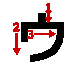
\includegraphics[trim= 00 05 00 00]{../share/katakana/us.pdf}
%\end{center}
\bigskip

\CharacterExplanation{us}{Write the first short strokes straight from up to
down. Then - and this is difficult place the second stroke in the correct
distance from the first one. Luckily this is also a straight stroke from up to
down. }

\bigskip

Of course the perception changes if the character is written in a square.
Remember that it is better to write the character in a square, because the
correct spaces between the character and the frame also determinates its
beauty.

\bigskip

\CharacterExplanation{uss}{The first stroke in the frame is not difficult as
mentioned before from straight up to down. However the frame helps because now
we understood that it is centered. The second stroke become also easier in a
frame because it is written at the edge of the character. After some time and
experience this is better understood. The last stroke has to join the first and
second stroke. That is still difficult with or without a frame.}

\bigskip

%----------------------------------------------------------------------------
\subsection{Stroke Types - 筆画の種類}

In European language there is no idea to have different stroke types unless one
enter the field of calligraphy. In Japanese there are different kind of
strokes.  Most important for Kanji, second important for Hiragana and least
important for Katakana since Katakana is also used for a bold replacement.  Due
to this fact the five different type of Japanese strokes ({筆画の種類}
{【ひっかくのしゅるい】}) will not repeated here. For now it is perfectly fine
to make all strokes equally thick. 



%\input{../share/sec/WritingKatakanaSentences}
\section{Special Katakana Characters}\jsec{特別カタカナ}
% [o] LABEL
\label{sec:SpecialKatakanaCharacters}
% [o] INDEX
\ifor{special Katakana characters}{特別カタカナ}{とくべつかたかな}{Spezielle Katakana Zeichen}
\ifor{Katakana}{片仮名}{かたかな}{Katakana}
\ifor{Gojūonzu}{五十音図}{ごじゅうおんず}{50 Laute Tafel}


As mentioned before \hyperref[sec:Katakana]{Katakana} is almost like Hiragana.
This is true for the \hyperref[sec:Gojuonzu]{Gojūonzu (50 sound table)  {五十音図}
{【ごじゅうおんず】}} This section will show the special characters, some are
different from the Hiragana set.

Special in some sense are characters used for punctuation, like {「。」},
{「!」} and {「?」}.  These are similar to the western counterparts but
differ a little bit. While it is obvious for the small circle {「。」}, also
{「!」} and {「?」} differ from the western equivalent in that sense that
they are \textbf{centerd} and occupy more (white) space. This characters among
other characters are used equally among Hiragana,
\hyperref[sec:Katakana]{Katakana} and Kanji. Therefore this section will not
further mention them.

%TODO check if point changes orientation and alignment in case of changing
%writing direction. 

\subsection{Doubling Vowels in Katakana}\jsubsec{カタカナでの倍増母音}
% [o] LABEL
\label{subsec:DoublingVowelsInKatakana}
\label{subsec:DoublingVowels}
\label{sec:DoublingVowelsInKatakana}
\label{sec:DoublingVowels}
% [o] INDEX
\ifor{doubling vowels}{倍増母音}{ばいぞうぼいん}{Vokalverdopplung}
\ifor{repition mark}{繰り返し記号}{くりかえしきごう}{Wiederholungszeichen}
\ifor{Katakana}{片仮名}{かたかな}{Katakana}

% カタカナでの倍増母音 【ばいぞうぼいん】

Special \hyperref[sec:Katakana]{Katakana} characters do also exists. The most
important character is Chōon {長音} {【ちょうおん】} the plain iteration
character {「ー」}, written as a stroke. It is one of the very few which
changes orientation according the writing orientation. When writing
\hyperref[sec:Katakana]{Katakana} from left to right the iteration character is
horizontal, while writing \hyperref[sec:Katakana]{Katakana} from up to down it
is vertical. The function of this character is to double the previous mora.
This is also different from Hiragana. (For doubling als other
\hyperref[sec:Katakana]{Katakana} caracter, refere to section
\nameref{sec:Iteration} on page \pageref{sec:Iteration}.)

\bigskip

\CharacterExplanation{k-iteration-s}{In standard gothic fonts the
\hyperref[sec:Katakana]{Katakana} iteration character is just a straight line
and it is not possible to understand in which direction it has to written. }

\bigskip

\CharacterExplanation{k-iteration-sm}{However if it is written with a different
font or with a brush it is clearly visible that in horizontal writing it is
written from left to right.} 

\bigskip


%\definecolor{orange}{rgb}{1,0.5,0}
%\definecolor{mygreen}{rgb}{.2,1,.2}

\bigskip
\textit{Example:}

\bigskip

\begin{center}
\begin{tabular}{p{7cm}p{7cm}}
Katakana:&Hiragana:\\
\Huge カ\textbf{\color{magenta}ー}ド /kaado/ &\Huge か\textbf{\color{magenta}あ}ど /kaado/\\
\end{tabular}
\end{center}

\bigskip

This character is very often used and makes \hyperref[sec:Katakana]{Katakana}
for this easier then Hiragana. The long vowel ambiguity do not exist.

As mentioned above the orientation of the \hyperref[sec:Katakana]{Katakana}
iteration character changes with the direction of writing. The above example
with different writing orientation.

\medskip
\textit{Example:}

\medskip

\begin{center}
\begin{tabular}{p{3.5cm}p{3.5cm}p{3.5cm}m{3.5cm}}
horizontally&
\setCJKfamilyfont{cjk-vert}[Script=CJK,RawFeature=horizontal]{IPAPGothic}
\mbox{
\begin{minipage}{3.2cm}
\Huge カ\textbf{\color{magenta}ー}ド
\end{minipage}
}
& vertically &
%\setCJKfamilyfont{cjk-vert}[Script=CJK,RawFeature=vertical]{Kozuka Gothic Pro M}
\setCJKfamilyfont{cjk-vert}[Script=CJK,RawFeature=vertical]{IPAPGothic}
\raisebox{-.5\height}{
\mbox{
\rotatebox{-90}{
\begin{minipage}{3.2cm} \CJKfamily{cjk-vert}
\Huge カ\textbf{\color{magenta}ー}ド
\end{minipage}
}
}
}
\\
\end{tabular}
\end{center}
\medskip



\subsection{Seldom Used Katakana}\jsubsec{めったに使われない片仮名}\label{subsec:SeldomlyUsedKatakana}

% めったに使われない片仮名 【めったにつかわれないかたかな】

Even though |wo| {「ヲ」}  is part if the standard letters. But since all
particle are written in Hiragana and in this case |wo| is written {「を」} the
learning of {「ヲ」} can be skipped. Unless it is important to read old texts,
like telegrams.



        % 2 chap:The Way to Write (Hiragana|Katakana)
    % +---------------------------------------------------------------------------+
% | english/chap/Pronunciation.tex                                            |
% |                                                                           |
% | Pronunciation of hiragana and katakana.                                   |
% |                                                                           |
% | Version: 0.1.3                                                            |
% |                                                                           |
% | Changes:                                                                  |
% |                                                                           |
% | 0.1.3 2024-03-28 Christian Külker <c@c8i.org>                             |
% |     - Fix typo                                                            |
% | 0.1.2 2023-06-05 Christian Külker <c@c8i.org>                             |
% |     - Improve English writing and paragraph about lexicon                 |
% | 0.1.1 2022-09-10 Christian Külker <c@c8i.org>                             |
% |     - Rename to english/chap/Pronunciation.tex                            |
% | 0.1.0 2020-07-10 Christian Külker <c@c8i.org>                             |
% |     - Initial release (as english/sec/KanaPronunciation.tex)              |
% |                                                                           |
% +---------------------------------------------------------------------------+
\chapter{Pronunciation}
\label{chap:Pronunciation}\label{sec:Pronunciation}

This chapter explains how to pronounce written Japanese with a focus on
\jkanavoc. After explaining the structure of pronunciation, it gives a detailed
view of intonation.

The \textbf{pronunciation} of \jkanavoc is exactly the same as for
\hyperref[sec:\jscript]{\jtopic}, and most sounds are very close to the Latin
\textbf{pronunciation}, but generally \textbf{pronounced} a little shorter
without any stress. Only the \jtl{ra} sounds, as in \jtl{ra}, \jtl{ri},
\jtl{ru}, \jtl{re} and \jtl{ro}, have no similarity in European languages.


The sound of the Japanese /r/ is  neither a central nor a lateral flap, but may
vary between the two. To an English speaker, its pronunciation varies between a
flapped 'd' (as in American English buddy) and a flapped 'l'.
\href{http://en.wikipedia.org/wiki/Japanese_phonology}{(Wikipedia Japanese
Phonology)}.


The following table shows the \textbf{pronunciation} in the
\hyperref[sec:Gojuonzu]{gojūonzu}.

\ien{Rōmaji Gojūonzu}
\ien{Rōmaji}
\ien{Gojūon}
\ija{ローマ字五十音図}
\ija{ローマ字}
\bigskip
\begin{center}
%\LARGE
%\Huge
\Padding
\begin{tabular}{c||c|c|c|c|c|}
&\textbf{a}&\textbf{i}&\textbf{u}&\textbf{e}&\textbf{o}\\\hline\hline
\textbf{-}&a&i&u&e&o\\\hline
\textbf{k}&ka&ki&ku&ke&ko\\\hline
\textbf{s}&sa&shi&su&se&so\\\hline
\textbf{t}&ta&chi&tsu&te&to\\\hline
\textbf{n}&na&ni&nu&ne&no\\\hline
\textbf{h}&ha&hi&fu&he&ho\\\hline
\textbf{m}&ma&mi&mu&me&mo\\\hline
\textbf{y}&ya&&yu&&yo\\\hline
\textbf{r}&ra&ri&ru&re&ro\\\hline
\textbf{w}&wa&&&&o\\\hline
\textbf{{*}}&n&&&&\\\hline
\end{tabular}
\end{center}


\section{Structure}

% Sound structure:
% - mora (haku,moora)
% - syllable

\textbf{Mora}, known in Japanese as \ivoc{haku}{拍}{はく}{Haku} or
\ivoc{モーラ}{モーラ}もおら{Mōra}, is similar to a
\hyperref[sec:Syllable]{syllable} and can be found in all languages. The plural
form of mora is \hyperref[sec:Mora]{morae}. A mora is a unit of time of fixed
length, equal to or shorter than a syllable. The structure of the spoken
Japanese language is based on morae rather than syllables.

In Japanese, each normal-sized kana is usually one mora. So-called constructed
sounds, which consist of a normal-sized kana and a small kana, are also one
mora. And there are some special moras that cannot be pronounced by themselves,
but still occupy a time slot. This means that, unlike English, the timing of
Japanese is equal and exact. Also unlike most European languages, writing and
mora have a fixed relation.

The two Japanese scripts \textbf{hiragana} and \textbf{katakana} are based on
morae. Therefore, instead of using the word letter, this book will use the
word mora when referring to a Japanese sound unit and its written
representation.

It is possible to write Japanese with our characters. We call our letters Latin
letters, while in Japan our letters are called Roman letters. Japanese
sentences look very similar to European languages when written with Latin
letters. Reading Japanese sentences with Roman characters has a major problem
with Japanese pronunciation. While English, German, French, and other European
languages are based on syllables, and syllables have different lengths,
Japanese morae have the same length.

For example, the English \jtl{i} and \jtl{shi} are of different lengths.
Transcribed into Japanese, \jtl{i} becomes \jquotesingleja{\jkanaletteri} and
\jtl{shi} becomes \jquotesingleja{\jkanalettershi}. Both are just a single
letter in the Japanese script \jtopic. An English speaker usually assumes that
\jtl{i} and \jtl{shi} have different lengths in pronunciation. In contrast, it
is natural for a Japanese speaker to assume that \jquotesingleja{\jkanaletteri}
and \jquotesingleja{\jkanalettershi} have the same length.

\section{Intonation}\jsec{イントネーション}

It is tempting to call the section on intonation "Eating Candy in the Rain" or
"Using Chopsticks on the Bridge"\footnote{The author talked about chopsticks in
Japanese with the correct intonation and got confused results while crossing a
bridge with a Japanese native in Chiba Prefecture in 1994.}. Two things to
avoid during a Japanese conversation.

\ifor{pronunciation}{発音}{はつおん}{Aussprache}
\ifor{intonation}{イントネーション}{いんとねーしょん}{Betonung}
\ifor{katakana}{片仮名}{かたかな}{Katakana}
\ifor{hiragana}{平仮名}{ひらがな}{Hiragana}
\ifor{mora}{モーラ}{もーら}{Mora}
\ifor{gojūonzu}{五十音図}{ごじゅうおんず}{50@50 Laute Tafel}

The \textbf{pronunciation} of \hyperref[sec:Hiragana]{hiragana} is the same as
for \hyperref[sec:Katakana]{katakana}. Therefore, each
\hyperref[sec:Syllable]{syllable}, more precisely each
\hyperref[sec:Mora]{mora}, corresponds to a \hyperref[sec:\jscript]{\jtopic}
character and is constructed as 'consonant' + 'vowel' with the exception of
\jtl{n}. This system of letters for each \hyperref[sec:Mora]{mora} makes
\textbf{pronunciation} absolutely clear without any ambiguity. However, the
simplicity of \hyperref[sec:\jscript]{\jtopic} does not mean that
\textbf{pronunciation} in Japanese is as easy for English speakers as it is for
Germans. The rigid structure of the fixed \hyperref[sec:Mora]{mora} sound in
Japanese creates the challenge of learning the correct intonation and duration
of Japanese \textbf{pronunciation}.

Almost every Japanese word can be broken down into \hyperref[sec:Mora]{morae}
of high and low pitch, which is a crucial aspect of the spoken language.
Compared to Chinese, Japanese fortunately has only two pitches: high and low.
This distinction in pitch is so significant in the Japanese language that even
words spelled identically in hiragana or katakana can have different meanings
based on their pitch patterns, warranting separate entries in the lexicon.
Further complicating this, words that are spelled the same way in kana can be
sometimes differentiated by their kanji writing. Even if they have the same or
different pitch patterns, different kanji representations give the words
distinct meanings, adding to the richness and complexity of the Japanese
lexicon. Therefore, understanding the nuances of pitch and word writing,
including the high and low pitch intonation and kanji usage, becomes an
essential aspect of mastering the spoken language.

{
\begin{table}[H]
  \begin{center}
    \setlength{\fboxsep}{.2ex}
    \bgroup
      \def\arraystretch{1.2}%  1 is the default
      \begin{tabular}{llllll}
        \textbf{English}&\textbf{Japanese}&
        \multicolumn{1}{p{2cm}}{\textbf{Intonation rōmaji}}&
        \multicolumn{1}{p{2cm}}{\textbf{Intonation hiragana}}&
        \multicolumn{1}{p{2cm}}{\textbf{Intonation katakana}}&\textbf{Remark}\\
        Rain    &雨      &\jtl{\jpitch[tr]{a}\jpitch[lb]{me}}&\jpitch[tr]{あ}\jpitch[lb]{め}&\jpitch[tr]{ア}\jpitch[lb]{メ}&\\
        Sky     &天      &\jtl{\jpitch[tr]{a}\jpitch[lb]{me}}&\jpitch[tr]{あ}\jpitch[lb]{め}&\jpitch[tr]{ア}\jpitch[lb]{メ}&\\
        Candy   &飴/あめ&\jtl{\jpitch[br]{a}\jpitch[lt]{me}}&\jpitch[br]{あ}\jpitch[lt]{め}&\jpitch[br]{ア}\jpitch[lt]{メ}&Usually kanji is not used\\
        American&アメ&\jtl{ame}&あ{ }め&ア{ }メ&Slang\\
      \end{tabular}
    \egroup
    \caption{Intonation of \jtl{ame}}
    \label{tab:IntonationOfAme}
  \end{center}
\end{table}
}

The \hyperref[tab:IntonationOfAme]{above} example of \jtl{ame} looks simple. A
given Japanese word with two morae can have one or the other intonation, or in
some cases none (either high or low). And it seems that a kanji can have only
one intonation per pronunciation. However, this is not true. A given kanji such
as \jquotesingleja{橋} \hyperref[tab:IntonationOfHashi]{for example} can have
more than one intonation, depending on its meaning and context.

{
\begin{table}[H]
  \begin{center}
    \setlength{\fboxsep}{.2ex}
    \bgroup
      \def\arraystretch{1.2}%  1 is the default
      \begin{tabular}{llllll}
        \textbf{English}&\textbf{Japanese}&
        \multicolumn{1}{p{2cm}}{\textbf{Intonation rōmaji}}&
        \multicolumn{1}{p{2cm}}{\textbf{Intonation hiragana}}&
        \multicolumn{1}{p{2cm}}{\textbf{Intonation katakana}}&\textbf{Remark}\\
        Edge     &端    &\jtl{\jpitch[br]{ha}\jpitch[lt]{shi}}&\jpitch[br]{は}\jpitch[lt]{し}&\jpitch[br]{ハ}\jpitch[lt]{シ}&\\
        Bridge   &橋    &\jtl{\jpitch[br]{ha}\jpitch[lt]{shi}}&\jpitch[br]{は}\jpitch[lt]{し}&\jpitch[br]{ハ}\jpitch[lt]{シ}&\\
        Hashi    &橋    &\jtl{\jpitch[tr]{ha}\jpitch[lb]{shi}}&\jpitch[tr]{は}\jpitch[lb]{し}&\jpitch[tr]{ハ}\jpitch[lb]{シ}&Family name\\
        Chopstick&箸    &\jtl{\jpitch[tr]{ha}\jpitch[lb]{shi}}&\jpitch[tr]{は}\jpitch[lb]{し}&\jpitch[tr]{ハ}\jpitch[lb]{シ}&Usually \jquotesingleja{お箸}\\
        Stairs   &階;梯&\jtl{\jpitch[tr]{ha}\jpitch[lb]{shi}}&\jpitch[tr]{は}\jpitch[lb]{し}&\jpitch[tr]{ハ}\jpitch[lb]{シ}&\\
        Beak     &嘴    &\jtl{\jpitch[tr]{ha}\jpitch[lb]{shi}}&\jpitch[tr]{は}\jpitch[lb]{し}&\jpitch[tr]{ハ}\jpitch[lb]{シ}&\\
        Persia   &波斯  &\jtl{\jpitch[tr]{ha}\jpitch[lb]{shi}}&\jpitch[tr]{は}\jpitch[lb]{し}&\jpitch[tr]{ハ}\jpitch[lb]{シ}&Old Chinese name of Iran\\
      \end{tabular}
    \egroup
    \caption{Intonation of \jtl{hashi}}
    \label{tab:IntonationOfHashi}
  \end{center}
\end{table}
}


Since Japanese is a context-sensitive language, be sure not to talk about candy
in the rain or chopsticks while crossing a bridge.

It is also true that intonation varies from area to area in Japan. The Tokyo
area is considered standard when it comes to intonation. Other areas may have
different intonation or the opposite intonation. When it comes to intonation
training, it is advisable to practice intonation with a native speaker from the
Kanto area or a person who speaks the standard intonation. However, if this is
not possible, the next best thing is to learn only \textbf{one} other
intonation and not a mixture of different intonations. If consistency in
intonation origin cannot be achieved, it may be better to skip the training
altogether.

One of the biggest problems in achieving a natural sounding
\textbf{pronunciation} is incorrect intonation. Many European or American
learners speak without paying attention to pitch. This makes the speech sound
unnatural to Japanese. Some language courses try to have the learner memorize
the natural pitch of a word or even teach memorization rules. While there is
clearly a way for linguistic rules to work, they are hard to remember and
master. It is still possible to learn the correct intonation by resorting to a
language learning technique used by infants and toddlers: imitating native
speakers. Therefore, it is highly recommended to listen to and imitate as much
spoken Japanese as possible. Radio, podcasts, plays, and television, to name a
few. However, it is not advisable to listen to too many artificial sources such
as anime or commercials.

\bigskip
\begin{tabular}{rl}
-&Every (yes \textbf{every}) \hyperref[sec:Mora]{mora} is \textbf{pronounced}
  with the same length\\
-&There are no short and long \hyperref[sec:Mora]{mora} or letters\\
-&Every \hyperref[sec:Mora]{mora} has a pitch: high or low\\
-&Every pitch matters\\
-&Pitch can sometimes change with its context\\
-&Pitch can change with a dialect - but standard Japanese has well-defined
  pitches\\
\end{tabular}

\bigskip

\section{Pronunciation}\jsec{発音}

        % 3 chap:Pronunciation
    % Training.tex: Training for hiragana and katakana
\ifthenelse{\equal{katakana}{\jtopic}}{%
\chapter{Katakana Training}\jchap{片仮名練習}\label{chap:KatakanaTraining}
\ithree{katakana!training}{片仮名練習}{Katakana!Training}
}{}
\ifthenelse{\equal{hiragana}{\jtopic}}{%
\chapter{Hiragana Training}\jchap{平仮名練習}\label{chap:HiraganaTraining}
\ithree{katakana!training}{平仮名練習}{Hiragana!Training}
}{}

\normalsize

Every person is learning in a different way. What works well for one does not
need to work well also for the other. Because of this an ultimate recipe to
learn \textbf{\jtopic} can not be given here. However the introduction to this
chapter would like to try to give some  hints gathered from learning and
teaching experience.

\begin{description}

\item[Not too less:] If one learns one character per day, it will take for
        \textbf{\jtopic} roughly \jkanacount{} days. If you restrict this to
        working days it will take approximately two month. If you restrict it
        to a 2h lesson per week it will take a year to learn \textbf{\jtopic}.
        It is obvious that one is likely to forget the first characters when
        learning the last. However, even with this method it is not impossible
        but not likely.

\item[Not too much:]  To learn \textbf{\jtopic} in one day is unlikely
        possible. At least parts will be forgotten the next day.

\end{description}

From the practice the best results have been seen when learners have tried to
learn \textbf{\jtopic} in one to three weeks. The suggestion is to learn one
line (five characters) per day in a cumulative way. Means, repeat every day the
already learned characters and that up to 10 days until all are learned. And
then repeat this exercise until they hardly can not be forgotten any more. So
for at least 14 consecutive days without break.

\begin{description}

\item[Develop your own style:] Learning one character at a time or a row (five
        characters at a time) or learn the whole table of \textbf{\jtopic} is
        possible. With some method it can take 3 weeks or with an other method
        1 week. That does not matter. What do matter is that oneself is
        comfortable with the method and that oneself extract fun out of it,
        even when forced to learn \textbf{\jtopic}. Decide by yourself how
        often you repeat. But decide. And write down your decision. Maybe even
        plan it in your daily plan. A good practice is to learn
        \textbf{\jtopic} 20 times a day for five minutes rather then one time
        for three hours a day or one time a week for 10 hours.

\item[Search for aid:] Aid can come in may manifestations. Of course it is
        useful to ask a Japanese to help. But there are many other ways for
        helping yourself.  One example are flashcards. Of course it is easy to
        print them in this book. However as said before: find your own way. And
        if you create flashcards by yourself you already learn the content up
        to a certain level.

\item[Use Squares:] Some European languages uses lines to teach letters. In
        Japanese you should use a square and draw the letter in the middle. If
        uncertain about the shape and orientation of the character use a square
        and look at the squares filled with \textbf{\jtopic} in this section to
        understand the alignment and orientation.

\end{description}

\newpage

Here are some examples for flashcards. But feel free to invent your own.

\begin{figure}[H]
        

\begin{center}
\begin{tabular}{cc}
\textbf{Front site rōmaji}&\textbf{Back site katakana}\\

\includegraphics[scale=1.5]{../share/i/fcar.pdf}% Rōmaji
&
\ifthenelse{\equal{hiragana}{\jtopic}}{
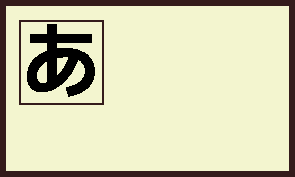
\includegraphics[scale=1.5]{../share/i/fcah.pdf}% Hiragana
}{}
\ifthenelse{\equal{katakana}{\jtopic}}{
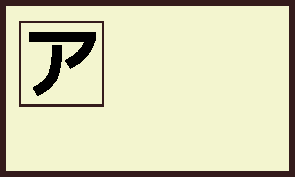
\includegraphics[scale=1.5]{../share/i/fcak.pdf}% Katakana
}{}
\\
\end{tabular}
\end{center}

        \caption{Flashcard type 1 (rōmaji - kana) }
        \label{fig:FlashCardTypeOne}
\end{figure}

\normalsize

Or to learn both:

\begin{figure}[H]
        \begin{center}
\begin{tabular}{cc}
\textbf{Front site rōmaji}&\textbf{Back site both}\\

\includegraphics[scale=1.5]{../share/i/fcar.pdf}% Rōmaji
&
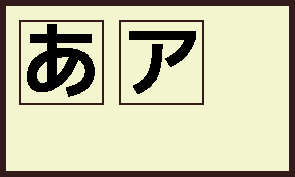
\includegraphics[scale=1.5]{../share/i/fcahk.pdf}% Hiragana/ Katakana
\\
\end{tabular}
\end{center}

        \caption{Flashcard type 2 (rōmaji - 2 kana)}
        \label{fig:FlashCardTypeTwo}
\end{figure}

\normalsize

To dive deep into Japanese of course skipping rōmaji is the preferred method:

\begin{figure}[H]
        \begin{center}
\begin{tabular}{cc}
\textbf{Front site Katakana}&\textbf{Back site Hiragana}\\
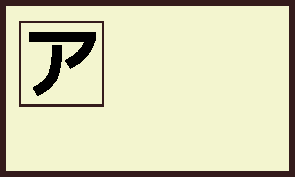
\includegraphics[scale=1.5]{../share/i/fcak.pdf}% Katakana
&
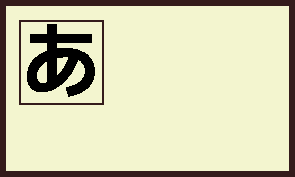
\includegraphics[scale=1.5]{../share/i/fcah.pdf}% Hiragana
\\
\end{tabular}
\end{center}

        \caption{Flashcard type 3 (katakana - hiragana)}
        \label{fig:FlashCardTypeThree}
\end{figure}

This training chapter can be used as an additional aid to learn
\textbf{\jtopic}. And also here it is important to develop ones own method.
However some hints on learning with this training chapter can be given.

\begin{description}

\item[Reading Loud:] While writing a \textbf{\jtopic} character in this book
        (and probably also later), read out loud the sound of the character.
        Always.

\item[Invent your own cribs:] One can (maybe should?) invent one crib per
        character by oneself. Especially if the characters is difficult to
        remember. It might be useful to write it down on the self created
        flashcard for that specific character.

\item[Regular Repetition:] It is of course possible to fill out all fields for
        one character in a very short time. The learning effect should be
        minimal though. Better is to fill out one row and then the second row
        an hour later, the third row the next day and so own. Oneself has to
        decide the rhythm of the repetition.

\item[Transcription:]  Search for a  \textbf{\jtopic} text and read it. Write
        for every \jtopic word the Roman letters. If this is possible without
        looking up the \jtopic, then the transcription should be reversed. Find
        some Japanese text written in Rōmaji and transcribe them to \jtopic on
        a different piece of paper.

\end{description}

\newpage

                                             % Katakana Hiragana
%----------------------------------------------------------------------------
\section{Katakana /a/ Row}\jsec{ 片仮名ア行}\label{sec:KatakanaARow}

\Krow{arow}{a}{i}{u}{e}{o}

\label{letter:a}\KLETTER{a} The 片仮名 {「ア」} derives from the
\hyperref[sec:PhoneticCharacter]{Phonetic Characters}
(\hyperref[sec:Radical]{radical}).  A smaller version {「ァ」} is used in
combinations with other letters as {「ファ」} and is pronounced as /fa/ in
\hyperref[sec:Hepburn]{Hepburn} transcription.

\label{letter:i}\KLETTER{i} The 片仮名 {「イ」} derives from the
\hyperref[sec:PhoneticCharacter]{Phonetic Characters} {「伊」} left element
(\hyperref[sec:Radical]{radical}).  A smaller version {「ィ」} is used in
combinations with other letters and represents a
\hyperref[sec:Diphthong]{diphthong}. 

\label{letter:u}\KLETTER{u} The 片仮名 {「ウ」} derives from the
\hyperref[sec:PhoneticCharacter]{Phonetic Character} {「宇」}. A smaller version
{「ゥ」} is used in combinations with other letters and represents a
\hyperref[sec:Diphthong]{diphthong} and is written as "w". Even though the
combination {「トゥ」} /tu/ exist, it is relatively new and many words do not
use it. In this cases {「ツ 」} /tsu/ is used. {「ウ」} can take
\hyperref[sec:Dakuten]{Dakuten} to form {「ヴ」} /vu/, which is relatively new
and can replace {「ブ」} /bu/. 

\Note{Note}{%

Be aware that the characters \hyperref[letter:fu]{「フ」},
\hyperref[letter:wa]{「ワ」}  and \hyperref[letter:u]{「ウ」} look very
similar.  Make sure that you spend extra training on distinguish them. 

}%


\newpage 

\label{letter:e}\KLETTER{e} The 片仮名 {「エ」} derives from the
\hyperref[sec:PhoneticCharacter]{Phonetic Characters} {「江」} right element
(\hyperref[sec:Radical]{radical}). A smaller version {「ェ」} is used in
combinations with other letters and express \hyperref[sec:Mora]{morae} of
foreign origin. For example {「ヴェ」} as pronounced /ve/.

\label{letter:o}\KLETTER{o} The 片仮名 {「オ」} derives from the
\hyperref[sec:PhoneticCharacter]{Phonetic Character} {「於」}. A smaller version
{「ォ」} is used in combinations with other letters and express
\hyperref[sec:Mora]{morae} of foreign origin. For example {「フォ 」} as
pronounced /fo/.

\newpage

% ---------------------------------------------------------------------------
\subsection{/a/}\jsubsec{「ア」} \label{sec:KatakanaA}

\KatakanaHeader{a}{ The Katakana {「ア」} is written with two strokes. The
first stroke starts horizontal. The second stroke is a curve with can be
attached to the first stroke in hand writing, but not at the horizontal part -
at the end of the first line.} \KatakanaTraining{a}

% ---------------------------------------------------------------------------
\subsection{/i/}\jsubsec{「イ」} \label{sec:KatakanaI}

\KatakanaHeader{i}{ The Katakana {「イ」} is written with one stroke. The first
stroke is a curve from upper right to lower left. The second stroke is a
vertical line attached to the first at the top.} \KatakanaTraining{i}

% ---------------------------------------------------------------------------
\subsection{/u/}\jsubsec{「ウ」} \label{sec:KatakanaU}

\KatakanaHeader{u}{The Katakana {「ウ」} is written with three strokes. The
first stroke a small vertical line. The second a small vertical line again and
the third line a horizontal line connection the two others.}
\KatakanaTraining{u}

% ---------------------------------------------------------------------------
\subsection{/e/}\jsubsec{「エ」} \label{sec:KatakanaE}

\KatakanaHeader{e}{The Katakana {「エ」} is written with three strokes. It is
very geometrically consisting only out of horizontal and vertical lines
connected together.} \KatakanaTraining{e}

% ---------------------------------------------------------------------------
\subsection{/o/}\jsubsec{「オ」} \label{sec:KatakanaO}

\KatakanaHeader{o}{The Katakana {「オ」} is written with three strokes. The
first line is horizontal and together with the second stroke it constructs a
perfect crossing. The third stroke beginning lies at the center of the
crossing.} \KatakanaTraining{o}

% ---------------------------------------------------------------------------
\subsection{/a/ Row Training}\jsubsec{片仮名ア行練習}
\Padding
\begin{longtable}[c]{p{2cm}p{2cm}p{3cm}p{6cm}p{2cm}}
\textit{Katakana}&\textit{Rōmaji}&\textit{Original}&\textit{Remark}&Origin\\\hline
ウエア&wuea&ware&          &English\\
エア  &ea  &air &          &English\\
エイ  &ei  &A   &the letter&English\\
\end{longtable}

\KanaSimpleTraining{Katakana to Rōmaji}{
\Transcribe{1.}{ウエア}{}{wear, ware}
\Transcribe{2.}{エア}{}{air}
\Transcribe{3.}{エイ}{}{A (the letter)}
\Transcribe{4.}{アイ}{}{I (the letter)}
\Transcribe{5.}{オウ}{}{O (the letter)}
%\Transcribe{6.}{イア}{}{ear}
}

\KanaSimpleTraining{Rōmaji to Katakana}{
\Transcribe{1.}{ea}{}{air}
\Transcribe{2.}{ai}{}{I (the letter)}
\Transcribe{3.}{ou}{}{O (the letter)}
\Transcribe{4.}{ei}{}{A (the letter)}
\Transcribe{5.}{uea}{}{wear, ware}
%\Transcribe{6.}{ia}{}{ear}
}

\newpage
\Padding
\begin{longtable}[c]{p{2cm}p{2cm}p{3cm}p{6cm}p{2cm}}
\textit{Katakana}&\textit{Rōmaji}&\textit{Original}&\textit{Remark}&Origin\\\hline
アイ  &ai  &I   &the letter&English\\
オウ  &ou  &O   &the letter&English\\
イア  &ia  &ear &          &English\\
\end{longtable}

\KanaSimpleTraining{English to Rōmaji}{
\Transcribe{1.}{ear}{}{}
\Transcribe{2.}{I (the letter)}{}{}
\Transcribe{3.}{air}{}{}
\Transcribe{4.}{O (the letter)}{}{}
\Transcribe{5.}{wear, ware}{}{}
%\Transcribe{6.}{A (the letter)}{}{}
}

\KanaSimpleTraining{English to Katakana}{
\Transcribe{1.}{I (the letter)}{}{}
\Transcribe{2.}{O (the letter)}{}{}
\Transcribe{3.}{air}{}{}
\Transcribe{4.}{ear}{}{}
\Transcribe{5.}{wear, ware}{}{}
%\Transcribe{6.}{A (the letter)}{}{}
}
\newpage
   % OK       OK
% ---------------------------------------------------------------------------
\section{Katakana \jtl{ka} Row}\jsec{片仮名カ行}\label{sec:KatakanaKaRow}

\Krow{karow}{ka}{ki}{ku}{ke}{ko}

\label{letter:ka}\KLETTER{ka} The  \textbf{katakana} \jquotesingleja{カ} is
pronounced \jtl{ka} and  derives from the
\hyperref[sec:PhoneticCharacter]{phonetic character}s \jquotesingleja{加} left
\hyperref[sec:Radical]{radical}.  A \hyperref[sec:Dakuten]{dakuten} version
exists and pronounced as \jtl{ga}.

%\hyperref[sec:Handakuten]{handakuten} does not exist in daily Japanese.
% \jquotesingleja{一ヵ所} {【いちかしょ】} (one place)
% \jquotesingleja{一ヶ所} {【いちかしょ】} (one place).
% 十ヵ条(十ヶ条)

\Note{Note}{

A smaller version \jquotesingleja{ヵ} is rare but used in combinations with
number particles.  For example in \jquotesingleja{一ヵ月} {【いっかげつ】} (one
month) and others.  This cases can also be written \jquotesingleja{一ヶ月}
{【いっかげつ】} (one month). Please see also \nameref{sec:KatakanaKe}. \Link
\href{https://ja.wikipedia.org/wiki/\%E3\%83\%B5}{ヵ}

}

\label{letter:ki}\KLETTER{ki} The \textbf{katakana} \jquotesingleja{キ} derives
from the \hyperref[sec:PhoneticCharacter]{phonetic character}s middle part of
either \jquotesingleja{機} or \jquotesingleja{幾}.  It is pronounced as
\jtl{ki}.  A \hyperref[sec:Dakuten]{dakuten} version exists and pronounced as
\jtl{gi}.


\label{letter:ku}\KLETTER{ku} The \textbf{katakana} \jquotesingleja{ク} derives
from the \hyperref[sec:PhoneticCharacter]{phonetic character}s left upper part
of \jquotesingleja{久}.  It is pronounced as \jtl{ku}.  A
\hyperref[sec:Dakuten]{dakuten} version exists and pronounced as \jtl{gu}.  A
smaller version exists, but is used for the Ainu Language.

\label{letter:ke}\KLETTER{ke} The \textbf{katakana} \jquotesingleja{ケ} derives
from the \hyperref[sec:PhoneticCharacter]{phonetic character}s upper and left
part of \jquotesingleja{介}.  It is pronounced as \jtl{ke}.  A
\hyperref[sec:Dakuten]{dakuten} version exists and pronounced as \jtl{ge}.  The
smaller version \jquotesingleja{ヶ} is explained in the following note.

\newpage

\Note{Note}{

A smaller version \jquotesingleja{ヶ} is rare but used in combinations with
number particles.  For example in \jquotesingleja{一ヶ月} {【いっかげつ】} (one
month) and others.  This cases can also be written \jquotesingleja{一ヵ月}
{【いっかげつ】} (one month). There are cases where only \jquotesingleja{ヶ}
can be written {七ヶ宿} {【シチカシュク】} (Place at the south west border of
the prefecture Miyagi).  In other rare cases this character can be pronounced
different \jquotesingleja{関ヶ原} {【せきがはら】} (Place at the south border
of the Gifu prefecture, known by the battle at 1600.). Please see also
\nameref{sec:KatakanaKa}. \Link
\href{https://ja.wikipedia.org/wiki/\%E3\%83\%B5}{ヵ}

}

\label{letter:ko}\KLETTER{ko} The \textbf{katakana} \jquotesingleja{コ} derives
from the \hyperref[sec:PhoneticCharacter]{phonetic character}s upper part of
\jquotesingleja{己}.  It is pronounced as \jtl{ko}.  A
\hyperref[sec:Dakuten]{dakuten} version exists and pronounced as \jtl{go}.



\newpage

% ---------------------------------------------------------------------------
\subsection{\jtl{ka}}\jsubsec{\jquotesingleja{カ}} \label{sec:KatakanaKa}

\KatakanaHeader{ka}{ \jtl{ka} is written with 2 strokes. Basically the same way
as the Hiragana \jquotesingleja{か} it looks like a squarish version, but
without the last stroke. The hook at the second stroke is less significant or
important.  } \KatakanaTraining{ka}

% ---------------------------------------------------------------------------
\subsection{\jtl{ki}}\jsubsec{\jquotesingleja{キ}} \label{sec:KatakanaKi}

\KatakanaHeader{ki}{ The shape alignment of the \jquotesingleja{キ} character
is not straight towards its environment. However the junctions are more or less
90 degrees.  } \KatakanaTraining{ki}

% ---------------------------------------------------------------------------
\subsection{\jtl{ku}}\jsubsec{\jquotesingleja{ク}} \label{sec:KatakanaKu}
% ---------------------------------------------------------------------------

\KatakanaHeader{ku}{ The first stroke is similar the stroke of
\jquotesingleja{ケ} is a curve. While the second stroke start aligned and
straight. } \KatakanaTraining{ku}

% ---------------------------------------------------------------------------
\subsection{\jtl{ke}}\jsubsec{\jquotesingleja{ケ}} \label{sec:KatakanaKe}

\KatakanaHeader{ke}{ The \jquotesingleja{ケ} is written with 3 strokes and the
first stroke is similar to the \jquotesingleja{ク}. The second stroke is
aligned and straight.  While the last stroke is a curve.  }
\KatakanaTraining{ke}

% ---------------------------------------------------------------------------
\subsection{\jtl{ko}}\jsubsec{\jquotesingleja{コ}} \label{sec:KatakanaKo}

\KatakanaHeader{ko}{ This character is almost a geometric figure composed out
of two strokes. However unless in European languages this are only 2 strokes
and not 3. The first stroke is the longest one and done similar with all
{漢字}. } \KatakanaTraining{ko}

% ---------------------------------------------------------------------------
\subsection{\jtl{ka} Row Training}\jsubsec{片仮名カ行練習}

\Padding
\begin{longtable}[c]{p{2cm}p{1.5cm}p{1.5cm}p{3cm}p{7cm}}
\textit{Katakana}&\textit{Rōmaji}&\textit{Original}&\textit{Remark}&Origin\\\hline
カキ  &kaki &kaki &柿 persimon&Japanese\\
ケア  &kea  &care &          &English\\
ケイ  &kei  &K    &the letter&English\\
\end{longtable}

\KanaSimpleTraining{Katakana to Rōmaji}{
\Transcribe{1.}{カキ}{}{persimmon}
\Transcribe{2.}{ココア}{}{cocoa}
\Transcribe{3.}{ケア}{}{care}
\Transcribe{4.}{コア}{}{core}
\Transcribe{5.}{ケーキ}{}{cake}
%\Transcribe{6.}{ケイ}{}{K (the letter)}
}

\KanaSimpleTraining{Rōmaji to Katakana}{
\Transcribe{1.}{kokoa}{}{cocoa}
\Transcribe{2.}{k$\overline{\mbox{e}}$ki}{}{cake}
\Transcribe{3.}{kea}{}{care}
\Transcribe{4.}{koa}{}{core}
\Transcribe{5.}{kaki}{}{persimmon}
%\Transcribe{6.}{kei}{}{K (the letter)}
}

\newpage

\Padding
%\begin{longtable}[c]{p{2cm}p{2cm}p{3cm}p{6cm}p{2cm}}
\begin{longtable}[c]{p{2cm}p{2.0cm}p{3.5cm}p{4cm}p{2.5cm}}
\textit{Katakana}&\textit{Rōmaji}&\textit{Original}&\textit{Remark}&Origin\\\hline
コア  &koa  &core &          &English\\
ココア&kokoa&cocoa& hot chocolate &English, from metathesis of Spanish cacao, from Nahuatl cacahuatl\\
ケーキ&kēki &cake &          &English\\
\end{longtable}


\KanaSimpleTraining{English to Rōmaji}{
\Transcribe{1.}{persimon}{}{}
\Transcribe{2.}{cocoa}{}{}
\Transcribe{3.}{care}{}{}
\Transcribe{4.}{core}{}{}
\Transcribe{5.}{K (the letter)}{}{}
%\Transcribe{6.}{cake}{}{}
}

\KanaSimpleTraining{English to Katakana}{
\Transcribe{1.}{cocoa}{}{}
\Transcribe{2.}{cake}{}{}
\Transcribe{3.}{care}{}{}
\Transcribe{4.}{persimon}{}{}
\Transcribe{5.}{K (the letter)}{}{}
%\Transcribe{6.}{core}{}{}
}

\newpage
  % OK
%----------------------------------------------------------------------------
\section{Katakana /sa/ Row}\jsec{片仮名サ行}\label{sec:KatakanaSaRow}

\Krow{sarow}{sa}{shi}{su}{se}{so}

\label{letter:sa}\KLETTER{sa} The  片仮名 {「サ」} is pronounced  /sa/ and
derives from the \hyperref[sec:PhoneticCharacter]{Phonetic Character}s {「散」}
upper left corner \hyperref[sec:Radical]{radical}.  A
\hyperref[sec:Dakuten]{濁点} version exists and pronounced as /za/.

\label{letter:shi}\KLETTER{shi} The 片仮名 {「シ」} derives from the
\hyperref[sec:PhoneticCharacter]{Phonetic Character}  {「之 」}.  It is
pronounced as /shi/.  A \hyperref[sec:Dakuten]{濁点} version exists and
pronounced as /ji/.

\Note{Note}{Please see section \nameref{subsec:ShiTsuAmbiguity} for the
explanation how to write and distinguish /shi/ and /tsu/.  }

\label{letter:su}\KLETTER{su} The 片仮名 {「ス」} derives from the
\hyperref[sec:PhoneticCharacter]{Phonetic Character}s right lower part of
{「須」}.  It is pronounced as /su/.  A \hyperref[sec:Dakuten]{濁点} version
exists and pronounced as /zu/.

\label{letter:se}\KLETTER{se} The 片仮名 {「セ」} derives from the
\hyperref[sec:PhoneticCharacter]{Phonetic Character}s middle left part of
{「世」}.  It is pronounced as /se/.  A \hyperref[sec:Dakuten]{濁点} version
exists and pronounced as /ze/.

\newpage

\label{letter:so}\KLETTER{so} The 片仮名 {「ソ」} derives from the
\hyperref[sec:PhoneticCharacter]{Phonetic Character}s upper right part of
{「曽」}.  It is pronounced as /so/.  A \hyperref[sec:Dakuten]{濁点} version
exists and pronounced as /zo/.

% SoRiNAmbiguity
\subsection{|so|, |ri| and |n| Ambiguity} \label{subsec:SoRiNAmbiguity}

The Katakana characters {「ソ」}, {「リ」} and {「ン」} can be difficult to
distinguish. All three are made out of only 2 strokes. And especially |so| and
|n| can be hard to tell. In a sentence of course the context can help a lot.
But what are the rules for this characters to write properly and distinguish?

\bigskip

\begin{center}
\begin{tabular}{|c|c|c|}\hline
\KLETTER{so}&\KLETTER{n}&\KLETTER{ri}\\\hline
\end{tabular}
\end{center}

\CharacterExplanation{soexplanation}{ To write the letter |so| it is important
to align both lines \textbf{horizontally} (red line) and to \textbf{non-align}
the ends (blue line) vertically. In this way it is possible to distinguish |so|
from |n|, but not from |ri|. To also distinguish it from |ri| you have to write
the first stroke not horizontally nor vertically (green line).  }

\CharacterExplanation{nexplanation}{ To write the letter |n| it is important to
a align both lines \textbf{vertically} (red line) and to \textbf{non-align} the
ends (blue line). In this way it is possible to distinguish |n| from |so|. If
both lines are aligned there should not be a problem to distinguish it from
|ri|. Usually the angle of the green line is different, but only a small
indicator. }

\CharacterExplanation{riexplanation}{ To write the letter |ri| it is important
to \textbf{align} both of the line beginnings \textbf{horizontally} (red line)
and to make sure that both lines are \textbf{parallel} (green lines). There
should be \textbf{no alignment} on the left side (blue line)
\textbf{vertically}. The difference between |so| and |ri| is that |ri| need to
start with two \textbf{parallel} lines wile |so| should not. Please compare the
left green line for an explanation.  }



\newpage
% ---------------------------------------------------------------------------
\subsection{/sa/}\jsubsec{「サ」}\label{sec:KatakanaSa}

\KatakanaHeader{sa}{ Katakana {「サ」} is written with three strokes. All
crossings of strokes are in a 90 degree angle.  The starts of all strokes are
aligned eitehr horizontally or vertically. The last stroke has a curve.}
\KatakanaTraining{sa}

% ---------------------------------------------------------------------------
\subsection{/shi/}\jsubsec{「シ」}\label{sec:KatakanaShi}

\KatakanaHeader{shi}{ The Katakana {「シ」} is written with three strokes. All
three strokes are aligned vertically in the beginning. Please see section
\nameref{subsec:ShiTsuAmbiguity}.} \KatakanaTraining{shi}

% ---------------------------------------------------------------------------
\subsection{/su/}\jsubsec{「ス」}\label{sec:KatakanaSu}

\KatakanaHeader{su}{The Katakana {「ス」} is written with two strokes. The
first stroke startes horizontally aligned. The second stroke touches the first
stroke at the beginning.} \KatakanaTraining{su}

% ---------------------------------------------------------------------------
\subsection{/se/}\jsubsec{「セ」}\label{sec:KatakanaSe}

\KatakanaHeader{se}{ The Katakana {「セ」} is written with two strokes. The
crossing has \textbf{no} 90 degree angle. The curve of the second stroke as
almost a 90 deegre angle. } \KatakanaTraining{se}

% ---------------------------------------------------------------------------
\subsection{/so/}\jsubsec{「ソ」}\label{sec:KatakanaSo}

\KatakanaHeader{so}{ The Katakana {「ソ」} is written with two strokes. The
first stroke is not aligned verticall but it is aligned horizontally withe the
second stroke. Please see section \nameref{subsec:SoRiNAmbiguity}.}
\KatakanaTraining{so}

% ---------------------------------------------------------------------------
\subsection{/sa/ Row Training}\jsubsec{片仮名サ行練習}\label{sec:SaRowTraining}
% 3 78 エキス
%3 357 スカイ
%3 360 スキー
%3 3 アイス
%3 111 ガーゼ
%3 146 イエス
\Padding
\begin{longtable}[c]{p{2cm}p{2cm}p{3cm}p{6cm}p{2cm}}
\textit{Katakana}&\textit{Rōmaji}&\textit{Original}&\textit{Remark}&\textit{Origin}\\\hline
エキス&ekisu&ex(tract)&extract&Dutch\\
スカイ&sukai&sky&&English\\
スキー&sukī&ski&noun for skiing&English\\
\end{longtable}
\KanaSimpleTraining{Katakana to Rōmaji}{
\Transcribe{1.}{エキス}{}{extract}      % ekisu
\Transcribe{2.}{スカイ}{}{sky}          % sukai
\Transcribe{3.}{スキー}{}{ski}          % sukī
\Transcribe{4.}{アイス}{}{ice}          % aisu
\Transcribe{5.}{ガーゼ}{}{gauze}        % gāze
%\Transcribe{6.}{イエス}{}{Jesus}        % iesu
}

\KanaSimpleTraining{Rōmaji to Katakana}{
\Transcribe{1.}{sukai}{}{sky}         % sukai
\Transcribe{2.}{ekisu}{}{extract}     % ekisu
\Transcribe{3.}{aisu}{}{ice}          % aisu
\Transcribe{4.}{suki}{}{ski}          % sukī
\Transcribe{5.}{iesu}{}{Jesus}        % iesu
%\Transcribe{6.}{gāze}{}{gauze}        % gāze
}

\newpage

\Padding
\begin{longtable}[c]{p{2cm}p{2cm}p{3cm}p{6cm}p{2cm}}
\textit{Katakana}&\textit{Rōmaji}&\textit{Original}&\textit{Remark}&Origin\\\hline
アイス&aisu&ice&water ice, ice cream&English\\
ガーゼ&gāze&Gaze&gauze&German\\
イエス&iesu&Jesus&Jesus&Portuguese\\
\end{longtable}
\KanaSimpleTraining{English to Rōmaji}{
\Transcribe{1.}{extract}{}{}       % ekisu
\Transcribe{2.}{sky}{}{}           % sukai
\Transcribe{3.}{Jesus}{}{}         % iesu
\Transcribe{4.}{gauze}{}{}         % gāze
\Transcribe{5.}{ice}{}{}           % aisu
%\Transcribe{6.}{ski}{}{}           % sukī
}

\KanaSimpleTraining{English to Katakana}{
\Transcribe{1.}{sky}{}{}           % sukai
\Transcribe{2.}{gauze}{}{}         % gāze
\Transcribe{3.}{ice}{}{}           % aisu
\Transcribe{4.}{Jesus}{}{}         % iesu
\Transcribe{5.}{extract}{}{}       % ekisu
%\Transcribe{6.}{ski}{}{}           % sukī
}

\newpage
  % OK
% ---------------------------------------------------------------------------
\section{Katakana \jtl{ta} Row}\jsec{片仮名タ行}\label{sec:KatakanaTaRow}

\Krow{tarow}{ta}{chi}{tsu}{te}{to}

\label{letter:ta}\KLETTER{ta} The  \textbf{katakana} \jquotesingleja{タ} is
pronounced \jtl{ta} and derives from the
\hyperref[sec:PhoneticCharacter]{phonetic character}s \jquotesingleja{多 }
upper or lover \hyperref[sec:Radical]{radical}.  A
\hyperref[sec:Dakuten]{dakuten} version exists and pronounced as \jtl{da}.

\label{letter:chi}\KLETTER{chi} The \textbf{katakana} \jquotesingleja{チ}
derives from the \hyperref[sec:PhoneticCharacter]{phonetic character} 
\jquotesingleja{千}.  It is pronounced as \jtl{chi}.  A
\hyperref[sec:Dakuten]{dakuten} version exists and pronounced as \jtl{ji}.

\label{letter:tsu}\KLETTER{tsu} The \textbf{katakana} \jquotesingleja{ツ}
derives from the \hyperref[sec:PhoneticCharacter]{phonetic character}s
\jquotesingleja{州} or \jquotesingleja{川} .  It is pronounced as \jtl{tsu}.  A
\hyperref[sec:Dakuten]{dakuten} version exists and pronounced as \jtl{zu}.

\label{letter:te}\KLETTER{te} The \textbf{katakana} \jquotesingleja{テ} derives
from the \hyperref[sec:PhoneticCharacter]{phonetic character}s lower left part
of \jquotesingleja{天 }.  It is pronounced as \jtl{te}.  A
\hyperref[sec:Dakuten]{dakuten} version exists and pronounced as \jtl{de}.

\newpage

\label{letter:to}\KLETTER{to} The \textbf{katakana} \jquotesingleja{ト} derives
from the \hyperref[sec:PhoneticCharacter]{phonetic character}s right part of
\jquotesingleja{止}.  It is pronounced as \jtl{to}.  A
\hyperref[sec:Dakuten]{dakuten} version exists and pronounced as \jtl{do}.

% ShiTsuAmbiguity
\subsection{|shi| and |tsu| Ambiguity} \label{subsec:ShiTsuAmbiguity}

% シ
% ツ

The Katakana characters {「シ」} and {「ツ」} are difficult to distinguish.
Both are made out of 3 strokes and even the length are equal. In a sentence of
course the context can help a lot. But what are the rules for this characters
to write properly and distinguish?

\bigskip

\begin{center}
\begin{tabular}{|c|c|}\hline
\KLETTER{shi}&\KLETTER{tsu}\\\hline
\end{tabular}
\end{center}

\CharacterExplanation{shiexplanation}{ To write the letter |shi| it is
important to align three lines \textbf{vertically} (red line) and to
\textbf{non-align} the ends (blue line). In this way it is possible to
distinguish |shi| from |tsu|. Of course also the angle of the frist two lines
are different, but in hadwriting this is difficult to match. As a rule of thumb
make the third line double as long as the first two but short enough to not
align it at the end. }

\CharacterExplanation{tsuexplanation}{ To write the letter |tsu| it is
important to align all tree lines \textbf{horizontally} (red line) and to
\textbf{non-align} the ends (blue line). In this way it is possible to
distinguish |tsu| from |shi|. Of course also the angle of the first two lines
are different, but in handwriting this is difficult to match. As a rule of
thumb make the third line double as long as the first two but short enough to
not align it at the end. }



\newpage

% ---------------------------------------------------------------------------
\subsection{\jtl{ta}}\jsubsec{\jquotesingleja{タ}}\label{sec:KatakanaTa}

\KatakanaHeader{ta}{ Katakana \jtl{ta} is written with three strokes. The first
stroke is a small curve. The secosnd stroke starts horizontally attached to the
first stroke. The third stroke ends at the second stroke.}
\KatakanaTraining{ta}

% ---------------------------------------------------------------------------
\subsection{\jtl{chi}}\jsubsec{\jquotesingleja{チ}}\label{sec:KatakanaChi}

\KatakanaHeader{chi}{ Katakana \jtl{chi} is written with three strokes. The
first stroke is a light curve. The second ihorizontally straight line. The
third line is a curve that joints the first and the second.}
\KatakanaTraining{chi}

% ---------------------------------------------------------------------------
\subsection{\jtl{tsu}}\jsubsec{\jquotesingleja{ツ}}\label{sec:KatakanaTsu}

\KatakanaHeader{tsu}{Katakana \jtl{tsu} is written with three strokes. The
first and second stroke are short. And the beginning of all three strokes is
aligned horizontally. The third stroke is the longest, but the end is not
alignd wit the beginning of the first stroke. } \KatakanaTraining{tsu}

% ---------------------------------------------------------------------------
\subsection{\jtl{te}}\jsubsec{\jquotesingleja{テ}}\label{sec:KatakanaTe}

\KatakanaHeader{te}{ Katakana \jtl{te} is written with three strokes. The first
stroke is the shortest and horizontally. The second stroke is not aligned
vertically in the beginning, but also perfectly horizontally. The third stroke
is a small curve attached to the middle of the second stroke. }
\KatakanaTraining{te}

% ---------------------------------------------------------------------------
\subsection{\jtl{to}}\jsubsec{\jquotesingleja{ト}}\label{sec:KatakanaTo}

\KatakanaHeader{to}{ Katakana \jtl{to} is written with 2 strokes. The first
stroke is a vertical line. Attached to this line there is short straight line
to the right. In some hand writings this line is a small curve to the right.}
\KatakanaTraining{to}

% ---------------------------------------------------------------------------
\subsection{\jtl{ta} Row Training}\jsubsec{片仮名タ行練習}
\Padding
\begin{longtable}[c]{p{2cm}p{2cm}p{3cm}p{6cm}p{2cm}}
\textit{Katakana}&\textit{Rōmaji}&\textit{Original}&\textit{Remark}&\textit{Origin}\\\hline
エステ        &esutei    &esthé(tique)&beauty salon, esthetic clinic    &French\\
サイト        &saito     &site        &&English\\
タスク        &tasuku    &task        &&English\\
\end{longtable}

\KanaSimpleTraining{Katakana to Rōmaji}{
\Transcribe{1.}{エステ}{}{esthé(tique)}
\Transcribe{2.}{サイト}{}{site}
\Transcribe{3.}{タスク}{}{task}
\Transcribe{4.}{テスト}{}{test}
\Transcribe{5.}{スーツアクター}{}{suit actor}
%\Transcribe{6.}{テキスト}{}{text}
}

\KanaSimpleTraining{Rōmaji to Katakana}{
\Transcribe{1.}{saito}{}{site}
\Transcribe{2.}{tasuku}{}{task}
\Transcribe{3.}{esute}{}{esthé(tique)}
\Transcribe{4.}{sūtsuakutā}{}{suit actor}
\Transcribe{5.}{tesuto}{}{test}
%\Transcribe{6.}{テキスト}{}{text}
}

\newpage
\Padding
\begin{longtable}[c]{p{2.6cm}p{2cm}p{1.8cm}p{6.6cm}p{1.8cm}}
\textit{Katakana}&\textit{Rōmaji}&\textit{Original}&\textit{Remark}&\textit{Origin}\\\hline
テスト        &tesuto    &test        &                                 &English\\
スーツアクター&sūtsuakutā&suit actor  &wearing cartoon-character costume&English\\
テキスト      &tekisuto  &text        &                                 &English\\
\end{longtable}

\KanaSimpleTraining{English to Rōmaji}{
\Transcribe{1.}{task}{}{}
\Transcribe{2.}{esthé(tique)}{}{}
\Transcribe{3.}{text}{}{}
\Transcribe{4.}{test}{}{}
\Transcribe{5.}{suit actor}{}{}
%\Transcribe{6.}{site}{}{}
}

\KanaSimpleTraining{English to Katakana}{
\Transcribe{2.}{esthé(tique)}{}{}
\Transcribe{4.}{test}{}{}
\Transcribe{5.}{suit actor}{}{}
\Transcribe{3.}{text}{}{}
\Transcribe{6.}{site}{}{}
%\Transcribe{1.}{task}{}{}
}

\newpage
  % OK
% ---------------------------------------------------------------------------
\section{Katakana \jtl{na} Row}\jsec{片仮名ナ行}\label{sec:KatakanaNaRow}

\Krow{narow}{na}{ni}{nu}{ne}{no}

\label{letter:na}\KLETTER{na} The  \textbf{katakana} \jquotesingleja{ナ} is
pronounced \jtl{na} and  derives from the
\hyperref[sec:PhoneticCharacter]{phonetic character}s \jquotesingleja{奈} upper
left corner part.  A \hyperref[sec:Dakuten]{dakuten} version  or
\hyperref[sec:Handakuten]{handakuten} do not exist.

\label{letter:ni}\KLETTER{ni} The  \textbf{katakana} \jquotesingleja{ニ} is
pronounced \jtl{ni} and  derives from the
\hyperref[sec:PhoneticCharacter]{phonetic character}s \jquotesingleja{奈} upper
right part.  A \hyperref[sec:Dakuten]{dakuten} version  or
\hyperref[sec:Handakuten]{handakuten} do not exist.

\label{letter:nu}\KLETTER{nu} The  \textbf{katakana} \jquotesingleja{ヌ} is
pronounced \jtl{nu} and  derives from the
\hyperref[sec:PhoneticCharacter]{phonetic character}s \jquotesingleja{奴} right
part.  A \hyperref[sec:Dakuten]{dakuten} version  or
\hyperref[sec:Handakuten]{handakuten} do not exist.

\Note{Note}{%


The characters \hyperref[letter:no]{「ノ」}, \hyperref[letter:me]{「メ」} and
\hyperref[letter:nu]{「ヌ」} are similar and it is easy to make a mistake. To
distinguish {「メ」} it is important to make all strokes long enough.}

}%


\newpage

\label{letter:ne}\KLETTER{ne} The  \textbf{katakana} \jquotesingleja{ネ} is
pronounced \jtl{ne} and  derives from the
\hyperref[sec:PhoneticCharacter]{phonetic character}s \jquotesingleja{祢} upper
left  part.  A \hyperref[sec:Dakuten]{dakuten} version  or
\hyperref[sec:Handakuten]{handakuten} do not exist.

\label{letter:no}\KLETTER{no} The  \textbf{katakana} \jquotesingleja{ノ} is
pronounced \jtl{no} and  derives from the
\hyperref[sec:PhoneticCharacter]{phonetic character}s \jquotesingleja{乃} upper
left part.  A \hyperref[sec:Dakuten]{dakuten} version  or
\hyperref[sec:Handakuten]{handakuten} do not exist.

\Note{Note}{%


The characters \hyperref[letter:no]{「ノ」}, \hyperref[letter:me]{「メ」} and
\hyperref[letter:nu]{「ヌ」} are similar and it is easy to make a mistake. To
distinguish {「メ」} it is important to make all strokes long enough.}

}%

\newpage

% ---------------------------------------------------------------------------
\subsection{\jtl{na}}\jsubsec{\jquotesingleja{ナ}} \label{sec:KatakanaNa}

\KatakanaHeader{na}{ Katakana \jtl{na} is written with two strokes.} \KatakanaTraining{na}

% ---------------------------------------------------------------------------
\subsection{\jtl{ni}}\jsubsec{\jquotesingleja{ニ}} \label{sec:KatakanaNi}

\KatakanaHeader{ni}{ Katakana \jtl{ni} is written with two strokes.} \KatakanaTraining{ni}

% ---------------------------------------------------------------------------
\subsection{\jtl{nu}}\jsubsec{\jquotesingleja{ヌ}} \label{sec:KatakanaNu}

\KatakanaHeader{nu}{Katakana \jtl{nu} is written with two strokes.} \KatakanaTraining{nu}

% ---------------------------------------------------------------------------
\subsection{\jtl{ne}}\jsubsec{\jquotesingleja{ネ}} \label{sec:KatakanaNe}

\KatakanaHeader{ne}{Katakana \jtl{ne} is written with three strokes.} \KatakanaTraining{ne}

% ---------------------------------------------------------------------------
\subsection{\jtl{no}}\jsubsec{\jquotesingleja{ノ}} \label{sec:KatakanaNo}

\KatakanaHeader{no}{Katakana \jtl{no} is written with one stroke.} \KatakanaTraining{no}

% ---------------------------------------------------------------------------
\subsection{ \jtl{na} Row Training}\jsubsec{片仮名ナ行練習}
\Padding
\begin{longtable}[c]{p{2cm}p{2cm}p{3cm}p{6cm}p{2cm}}
\textit{Katakana}&\textit{Rōmaji}&\textit{Original}&\textit{Remark}&\textit{Origin}\\\hline
ナース  &nāsu &nurse      &                                        &English\\
ネット  &netto&net(work)  &                                        &English\\
アニス &anisu&anise      &pimpinella anisum                       &\\
\end{longtable}

\KanaSimpleTraining{Katakana to Rōmaji}{
\Transcribe{1.}{ネット}{}{net(work)}
\Transcribe{2.}{ナース}{}{nurse}
\Transcribe{3.}{アニス}{}{anise}
\Transcribe{4.}{ニート}{}{NEET}
\Transcribe{5.}{ナイター}{}{night + -er}
%\Transcribe{6.}{ノート}{}{note}
}

\KanaSimpleTraining{Rōmaji to Katakana}{
\Transcribe{1.}{nōto}{}{note}
\Transcribe{2.}{netto}{}{net(work)}
\Transcribe{3.}{anisu}{}{anise}
\Transcribe{4.}{nāsu}{}{nurse}
\Transcribe{5.}{naitā}{}{night + -er}
%\Transcribe{4.}{ニート}{}{NEET}
}

\newpage
\Padding
\begin{longtable}[c]{p{2cm}p{2cm}p{3cm}p{6cm}p{2cm}}
\textit{Katakana}&\textit{Rōmaji}&\textit{Original}&\textit{Remark}&\textit{Origin}\\\hline
ニート  &nīto &NEET       &Not in Education, Employment or Training&English\\
ナイター&naitā&night + -er&     a night game                       &English\\
ノート  &nōto &note       & note, notebook                         &English\\
\end{longtable}
\KanaSimpleTraining{English to Rōmaji}{
\Transcribe{1.}{anise}{}{}
\Transcribe{2.}{net(work)}{}{}
\Transcribe{3.}{note}{}{}
\Transcribe{4.}{nurse}{}{}
\Transcribe{5.}{NEET}{}{}
%\Transcribe{5.}{night + -er}{}{}
}

\KanaSimpleTraining{English to Katakana}{
\Transcribe{1.}{nurse}{}{}
\Transcribe{2.}{note}{}{}
\Transcribe{3.}{net(work)}{}{}
\Transcribe{4.}{anise}{}{}
\Transcribe{5.}{night + -er}{}{}
%\Transcribe{4.}{NEET}{}{}
}

\newpage
  %
% ---------------------------------------------------------------------------
\section{ Katakana \jtl{ha} Row}\jsec{片仮名ハ行}\label{sec:KatakanaHaRow}

\Krow{harow}{ha}{hi}{fu}{he}{ho}

\label{letter:ha}\KLETTER{ha} The \textbf{katakana} \jquotesingleja{ハ} is
pronounced \jtl{ha} and derives from the
\hyperref[sec:PhoneticCharacter]{phonetic character} \jquotesingleja{八 }.  A
\hyperref[sec:Dakuten]{dakuten} version exists and pronounced as \jtl{ba}.

\label{letter:hi}\KLETTER{hi} The \textbf{katakana} \jquotesingleja{ヒ} derives
from the \hyperref[sec:PhoneticCharacter]{phonetic characters}
\jquotesingleja{比} reight \hyperref{sec:Radical}{radical}. It is pronounced as
\jtl{hi}. A \hyperref[sec:Dakuten]{dakuten} version exists and pronounced as
\jtl{bi}.

\label{letter:fu}\KLETTER{fu} The \textbf{katakana} \jquotesingleja{フ} derives
from the \hyperref[sec:PhoneticCharacter]{phonetic characters} upper left part
of \jquotesingleja{不 }. It is pronounced as \jtl{fu}. A
\hyperref[sec:Dakuten]{dakuten} version exists and pronounced as \jtl{bu}.

\label{letter:he}\KLETTER{he} The \textbf{katakana} \jquotesingleja{ヘ} derives
from the \hyperref[sec:PhoneticCharacter]{phonetic characters} right
\hyperref{sec:Radical}{radical} of \jquotesingleja{部}. It is pronounced as
\jtl{he}. A \hyperref[sec:Dakuten]{dakuten} version exists and pronounced as
\jtl{be}.

\Warn{Warning}{The Katakana \jquotesingleja{ヘ} is the same character as the
        \hyperref[sec:Hiragana]{hiragana} \jquotesingleja{へ}. In some
        documents they can be distinguished because the font is different.
        However in genral they are the same. }

\label{letter:ho}\KLETTER{ho} The \textbf{katakana} \jquotesingleja{ホ} derives
from the \hyperref[sec:PhoneticCharacter]{phonetic characters} lower right part
of \jquotesingleja{保} wich by itself is the \hyperref[sec:Radical]{radical}
and \hyperref[sec:Kanji]{kanji} of tree. It is pronounced as \jtl{ho}. A
\hyperref[sec:Dakuten]{dakuten} version exists and pronounced as \jtl{bo}.

% UFuWaSimilarity
\subsection{|u|, |fu| and |wa| Similarity} \label{subsec:UFuWaSimilarity}

The Katakana characters {「ウ」}, {「フ」} and {「ワ」} can be easily
distinguished. All three have a different stroke count. However the shape is
similar. Therefore they can be mistaken. Especially when they have no context. 

\bigskip

\begin{center}
\begin{tabular}{|c|c|c|}\hline
\KLETTER{u}&\KLETTER{fu}&\KLETTER{wa}\\\hline
\end{tabular}
\end{center}




\newpage

% ハヒフヘホ
% ---------------------------------------------------------------------------
\subsection{\jtl{ha}}\jsubsec{\jquotesingleja{ハ}} \label{sec:KatakanaHa}

\KatakanaHeader{ha}{ The Katakana \jquotesingleja{ハ} is written with two
strokes. Non of them is striaght.} \KatakanaTraining{ha}

% ---------------------------------------------------------------------------
\subsection{\jtl{hi}}\jsubsec{\jquotesingleja{ヒ}} \label{sec:KatakanaHi}

\KatakanaHeader{hi}{ The Katakana \jquotesingleja{ヒ} is written with two
strokes. One stroke from right to left. The other stroke from up to down and
then a curve.  The difficulty of this character is to hit the first stroke with
the second. } \KatakanaTraining{hi}

% ---------------------------------------------------------------------------
\subsection{\jtl{fu}}\jsubsec{\jquotesingleja{フ}} \label{sec:KatakanaFu}

\KatakanaHeader{fu}{The pronuciation of Katakana \jquotesingleja{フ} is
\textbf{not} \jtl{hu} it is \jtl{fu} and it is written with only one stroke. }
\KatakanaTraining{fu}

% ---------------------------------------------------------------------------
\subsection{\jtl{he}}\jsubsec{\jquotesingleja{ヘ}} \label{sec:KatakanaHe}

\KatakanaHeader{he}{Katakana \jquotesingleja{ヘ} is written with one stroke
from left to right. This is the same character as
\hyperref[sec:Hiragana]{hiragana} \jtl{he}.} \KatakanaTraining{he}

% ---------------------------------------------------------------------------
\subsection{\jtl{ho}}\jsubsec{\jquotesingleja{ホ}} \label{sec:KatakanaHo}

\KatakanaHeader{ho}{The Kataka \jquotesingleja{ホ} character reminds at the
        Kanji for tree and is also written in the same order and with the same
        amount of stroke.  However the left and righ 'root' is not connected to
        the base. In cursive writing the character is written with a
hook-stroke as the second stroke. This is abstract available even in the bold
form where the second stroke has a small curve at the end.}
\KatakanaTraining{ho}

% ---------------------------------------------------------------------------
\subsection{\jtl{ha} Row Training}\jsubsec{片仮名ハ行練習}\label{sec:HaRowTraining}
\Padding
\begin{longtable}[c]{p{3cm}p{2cm}p{3cm}p{5cm}p{2cm}}
\textit{Katakana}&\textit{Rōmaji}&\textit{Original}&\textit{Remark}&\textit{Origin}\\\hline
ホットケーキ&hottokēki&hotcake    &a pancake                         &English\\
コーヒー    &kōhī     &koffie     &珈琲  coffee                      &Dutch\\
ソフト      &sofuto   &soft(ware) &                                  &English \\
\end{longtable}

\KanaSimpleTraining{Katakana to Rōmaji}{
\Transcribe{1.}{ホットケーキ}{}{hotcake}
\Transcribe{2.}{コーヒー}{}{coffee}
\Transcribe{3.}{ソフト}{}{soft(ware)}
\Transcribe{4.}{ハイタッチ}{}{high five}
\Transcribe{5.}{ハウス}{}{house}
%\Transcribe{6.}{ハイネック}{}{high neck}
}

\KanaSimpleTraining{Rōmaji to Katakana}{
\Transcribe{1.}{kōhī}{}{coffee}
\Transcribe{2.}{hottokēki}{}{hotcake}
\Transcribe{3.}{haitacchi}{}{high five}
\Transcribe{4.}{sofuto}{}{soft(ware)}
\Transcribe{5.}{hainekku}{}{high neck}
%\Transcribe{6.}{hausu}{}{house}
}

\newpage
\Padding
\begin{longtable}[c]{p{2cm}p{2cm}p{3cm}p{6cm}p{2cm}}
\textit{Katakana}&\textit{Rōmaji}&\textit{Original}&\textit{Remark}&\textit{Origin}\\\hline
ハイタッチ  &haitacchi&high touch &high five                         &English\\
ハウス      &hausu    &Haus, house&                                  &English, German\\
ハイネック  &hainekku &high neck  &turtle neck style sweater or shirt&English\\
\end{longtable}
\KanaSimpleTraining{English to Rōmaji}{
\Transcribe{1.}{coffee}{}{}
\Transcribe{2.}{hotcake}{}{}
\Transcribe{3.}{high five}{}{}
\Transcribe{4.}{software}{}{}
\Transcribe{5.}{high neck}{}{}
%\Transcribe{6.}{house}{}{}
}

\KanaSimpleTraining{English to Katakana}{
\Transcribe{1.}{hotcake}{}{}
\Transcribe{2.}{high five}{}{}
\Transcribe{3.}{coffee}{}{}
\Transcribe{4.}{high neck}{}{}
\Transcribe{5.}{house}{}{}
%\Transcribe{6.}{software}{}{}
}

\newpage
  % OK
% ---------------------------------------------------------------------------
\section{Katakana /ma/ Row}\jsec{片仮名マ行}\label{sec:KatakanaMaRow}

\Krow{marow}{ma}{mi}{mu}{me}{mo}

\label{letter:ma}\KLETTER{ma} The  片仮名 {「マ」} is pronounced  /ma/ and
derives from the \hyperref[sec:PhoneticCharacter]{Phonetic Character}s {「末」}
upper two parallel horizontal strokes.  A \hyperref[sec:Dakuten]{濁点} or
\hyperref[sec:Handakuten]{半濁点} version do not exist.

\label{letter:mi}\KLETTER{mi} The  片仮名 {「ミ」} is pronounced  /mi/ and
derives from the \hyperref[sec:PhoneticCharacter]{Phonetic Character} {「三」}.
A \hyperref[sec:Dakuten]{濁点} or \hyperref[sec:Handakuten]{半濁点} version do
not exist.

\label{letter:mu}\KLETTER{mu} The  片仮名 {「ム」} is pronounced  /mu/ and
derives from the \hyperref[sec:PhoneticCharacter]{Phonetic Character}s {「牟
」} upper part.  A \hyperref[sec:Dakuten]{濁点} or
\hyperref[sec:Handakuten]{半濁点} version do not exist.

\newpage

\label{letter:me}\KLETTER{me} The  片仮名 {「メ」} is pronounced  /me/ and
derives from the \hyperref[sec:PhoneticCharacter]{Phonetic Character}s {「女」}
ilower right part.  A \hyperref[sec:Dakuten]{濁点} or
\hyperref[sec:Handakuten]{半濁点} version do not exist.

\Note{Note}{%


The characters \hyperref[letter:no]{「ノ」}, \hyperref[letter:me]{「メ」} and
\hyperref[letter:nu]{「ヌ」} are similar and it is easy to make a mistake. To
distinguish {「メ」} it is important to make all strokes long enough.}

}%


\label{letter:mo}\KLETTER{mo} The  片仮名 {「モ」} is pronounced  /mo/ and
derives from the \hyperref[sec:PhoneticCharacter]{Phonetic Character}s {「毛」}
ilower part exluding the first stroke.  A \hyperref[sec:Dakuten]{濁点} or
\hyperref[sec:Handakuten]{半濁点} version do not exist.

\newpage

\subsection{/ma/}\jsubsec{「マ」} \label{sec:KatakanaMa}

\KatakanaHeader{ma}{ Katakana /ma/ is written with three strokes.}
\KatakanaTraining{ma}

\subsection{/mi/}\jsubsec{「ミ」} \label{sec:KatakanaMi}

\KatakanaHeader{mi}{ Katakana /mi/ is written with three strokes.}
\KatakanaTraining{mi}

\subsection{/mu/}\jsubsec{「ム」} \label{sec:KatakanaMu}

\KatakanaHeader{mu}{ Katakana /mu/ is written with three strokes.}
\KatakanaTraining{mu}

\subsection{/me/}\jsubsec{「メ」/} \label{sec:KatakanaMe}

\KatakanaHeader{me}{ Katakana /me/ is written with three strokes.}
\KatakanaTraining{me}

\subsection{/mo/}\jsubsec{「モ」} \label{sec:KatakanaMo}

\KatakanaHeader{mo}{ Katakana /mo/ is written with three strokes.}
\KatakanaTraining{mo}

\subsection{/ma/ Row Training}\jsubsec{片仮名マ行練習}
\Padding
\begin{longtable}[c]{p{2cm}p{1.5cm}p{2.5cm}p{3cm}p{5cm}}
\textit{Katakana}&\textit{Rōmaji}&\textit{Original}&\textit{Remark}&Origin\\\hline
テーマ  &tēma    &Thema                 &theme                 &German\\
ママ    &mama    &mamá                  &mom                   &Spanish\\
ホーム  &hōmu    &(plat)form            &railway platform      &English\\
\end{longtable}

%シーエム        shīemu    C.M. (Commercial Message)       television commercial   English
%アニメ          anime     anima(tion)                  animated cartoons or films English

\KanaSimpleTraining{Katakana to Rōmaji}{
\Transcribe{1.}{テーマ}{}{theme}
\Transcribe{2.}{ママ}{}{mom}
\Transcribe{3.}{ホーム}{}{railway platform }
\Transcribe{4.}{アメフト}{}{American football}
\Transcribe{5.}{ハモる}{}{to harmonize (singing)}
%\Transcribe{6.}{マスコミ}{}{mass media}
}

\KanaSimpleTraining{Rōmaji to Katakana}{
\Transcribe{1.}{mama}{}{mom}
\Transcribe{2.}{tēma}{}{theme}
\Transcribe{3.}{amefuto}{}{American football}
\Transcribe{4.}{masukomi}{}{mass media}
\Transcribe{5.}{hōmu}{}{railway platform }
%\Transcribe{6.}{hamoru}{}{to harmonize (singing)}
}

\newpage
\Padding
\begin{longtable}[c]{p{2cm}p{2cm}p{4cm}p{4cm}p{3cm}}
\textit{Katakana}&\textit{Rōmaji}&\textit{Original}&\textit{Remark}&Origin\\\hline
アメフト&amefuto &Ame(rican) foot(ball) &American football     &English\\
ハモる  &hamoru  &harmo(ny) + -ru       &to harmonize (singing)&English, Japanese\\
マスコミ&masukomi&mass communication    &mass media            &English\\
\end{longtable}
\KanaSimpleTraining{English to Rōmaji}{
\Transcribe{1.}{theme}{}{}
\Transcribe{2.}{American football}{}{}
\Transcribe{2.}{mom}{}{}
\Transcribe{3.}{to harmonize (singing)}{}{}
\Transcribe{4.}{railway platform }{}{}
%\Transcribe{5.}{mass media}{}{}
}

\KanaSimpleTraining{English to Katakana}{
\Transcribe{1.}{American football}{}{}
\Transcribe{2.}{mom}{}{}
\Transcribe{3.}{railway platform }{}{}
\Transcribe{4.}{theme}{}{}
\Transcribe{5.}{mass media}{}{}
%\Transcribe{6.}{to harmonize (singing)}{}{}
}

\newpage
  %
% ---------------------------------------------------------------------------
\section{Katakana \jtl{ya} Row}\jsec{片仮名ヤ行}\label{sec:KatakanaYaRow}

\Krow{yarow}{ya}{s}{yu}{s}{yo}

\KLETTER{ya} The  \textbf{katakana} \jquotesingleja{ヤ} is pronounced  \jtl{ya}
and  derives from the \hyperref[sec:PhoneticCharacter]{phonetic character}s
\jquotesingleja{也} upper left part.  A \hyperref[sec:Dakuten]{dakuten} or
\hyperref[sec:Handakuten]{handakuten} version do not exist.

\KLETTER{yu} The  \textbf{katakana} \jquotesingleja{ユ} is pronounced  \jtl{yu}
and  derives from the \hyperref[sec:PhoneticCharacter]{phonetic character}s
\jquotesingleja{由 } lower middle part.  A \hyperref[sec:Dakuten]{dakuten} or
\hyperref[sec:Handakuten]{handakuten} version do not exist.

\KLETTER{yo} The  \textbf{katakana} \jquotesingleja{ヨ} is pronounced  \jtl{yo}
and  derives from the \hyperref[sec:PhoneticCharacter]{phonetic character}s
\jquotesingleja{與} upper right part.  A \hyperref[sec:Dakuten]{dakuten} or
\hyperref[sec:Handakuten]{handakuten} version do not exist.

\newpage
\subsection{Yōon}\jsubsec{拗音}

All characters from the \jquotesingleja{ヤ} row can be used in it's smaller form to crate
combined phonetics Yōon ({拗音} {【ようおん】}).

\begin{center} \Large
\begin{tabular}{llll}
      &ャ  &ュ  &ョ  \\
k - キ&キャ&キュ&キョ\\
s - シ&シャ&シュ&ショ\\
c - チ&チャ&チュ&チョ\\
n - ニ&ニャ&ニュ&ニョ\\
h - ヒ&ヒャ&ヒュ&ヒョ\\
m - ミ&ミャ&ミュ&ミョ\\
r - リ&リャ&リュ&リョ\\
\end{tabular}

Dakuten

\begin{tabular}{llll}
g - ギ&ギャ&ギュ&ギョ\\
j - ジ&ジャ&ジュ&ジョ\\
b - ビ&ビャ&ビュ&ビョ\\
\end{tabular}

Handakuten

\begin{tabular}{llll}
p - ピ&ピャ&ピュ&ピョ\\
\end{tabular}
\end{center}


\newpage

%ヤユヨ
\subsection{\jtl{sa}}\jsubsec{\jquotesingleja{ヤ}}\label{sec:KatakanaYa}

\KatakanaHeader{ya}{ Katakana \jtl{ya} is written with two strokes.} \KatakanaTraining{ya}

\subsection{\jtl{yu}}\jsubsec{\jquotesingleja{ユ}}\label{sec:KatakanaYu}

\KatakanaHeader{yu}{ Katakana \jtl{yu} is written with two strokes.} \KatakanaTraining{yu}

\subsection{\jtl{yo}}\jsubsec{\jquotesingleja{ヨ}}\label{sec:KatakanaYo}

\KatakanaHeader{yo}{Katakana \jtl{yo} is written with three strokes.} \KatakanaTraining{yo}

\subsection{\jtl{ya} Row Training}\jsubsec{片仮名ヤ行練習}
\Padding
\begin{longtable}[c]{p{2cm}p{1.5cm}p{2.5cm}p{3cm}p{6cm}}
\textit{Katakana}&\textit{Rōmaji}&\textit{Original}&\textit{Remark}&Origin\\\hline
イヤー              &iyā          &ear, year    &                         &English\\
ユーザー            &yūzā         &user         &                         &English\\
ヨード              &yōdo         &Jod          &iodine                   &German\\
\end{longtable}

\KanaSimpleTraining{Katakana to Rōmaji}{
\Transcribe{1.}{イヤー}{}{ear, year}
\Transcribe{2.}{ユーザー}{}{user}
\Transcribe{3.}{ヨード}{}{iodine}
\Transcribe{4.}{ユニットバス}{}{unit bath}
\Transcribe{5.}{ヨット}{}{sailboat}
\Transcribe{6.}{ニュー・イヤーズ・イブ}{}{new years eve}
}

\KanaSimpleTraining{Rōmaji to Katakana}{
\Transcribe{1.}{yūzā}{}{user}
\Transcribe{2.}{iyā}{}{ear, year}
\Transcribe{3.}{yunittobasu}{}{unit bath}
\Transcribe{4.}{yōdo}{}{iodine}
\Transcribe{5.}{nyū iyāzu ibu}{}{new years eve}
%\Transcribe{6.}{yotto}{}{sailboat}
}

\newpage
\Padding
\begin{longtable}[c]{p{3.9cm}p{2.4cm}p{2.6cm}p{4.8cm}p{1.3cm}}
\textit{Katakana}&\textit{Rōmaji}&\textit{Original}&\textit{Remark}&Origin\\\hline
ユニットバス        &yunittobasu  &unit bath    &prefabricated module bath&English\\
ヨット              &yotto        &yacht        &sailboat                 &English\\
ニュー・イヤーズ・イブ&nyū iyāzu ibu&new years eve&                         &English\\
\end{longtable}

\KanaSimpleTraining{English to Rōmaji}{
\Transcribe{3.}{unit bath}{}{}
\Transcribe{4.}{iodine}{}{}
\Transcribe{5.}{new years eve}{}{}
\Transcribe{1.}{user}{}{}
\Transcribe{6.}{sailboat}{}{}
%\Transcribe{2.}{ear, year}{}{}
}

\KanaSimpleTraining{English to Katakana}{
\Transcribe{1.}{sailboat}{}{}
\Transcribe{2.}{iodine}{}{}
\Transcribe{3.}{new years eve}{}{}
\Transcribe{4.}{unit bath}{}{}
\Transcribe{5.}{user}{}{}
%\Transcribe{2.}{ear, year}{}{}
}

\newpage
  %
% ---------------------------------------------------------------------------
\section{Katakana \jtl{ra} row}\jsec{片仮名ラ行}\label{sec:KatakanaRaRow}

\Krow{rarow}{ra}{ri}{ru}{re}{ro}

\KLETTER{ra} The  \textbf{katakana} \jquotesingleja{ラ} is pronounced  \jtl{ra}
(flapped 'r') and  derives from the \hyperref[sec:PhoneticCharacter]{phonetic
character}s \jquotesingleja{良} upper right corner part.  A
\hyperref[sec:Dakuten]{dakuten}  or \hyperref[sec:Handakuten]{handakuten}
version  do not exist.

\Note{Note}{

The sound of the Japanese /r/ is  neither a central nor a lateral flap, but may
vary between the two. To an English speaker, its pronunciation varies between a
flapped 'd' (as in American English buddy) and a flapped 'l'.
\href{http://en.wikipedia.org/wiki/Japanese_phonology}{(Wikipedia Japanese
Phonology)}.

}

\KLETTER{ri} The  \textbf{katakana} \jquotesingleja{リ} is pronounced  \jtl{ri}
(flapped 'r') and  derives from the \hyperref[sec:PhoneticCharacter]{phonetic
character}s \jquotesingleja{利}  right site part.  A
\hyperref[sec:Dakuten]{dakuten}  or \hyperref[sec:Handakuten]{handakuten}
version  do not exist.

%\Note{Note}{Please see section \nameref{subsec:SoRiNAmbiguity} for the explanation
%how to write and distinguish \jtl{so}, \jtl{n} and \jtl{ri}.
%}

\KLETTER{ru} The  \textbf{katakana} \jquotesingleja{ル} is pronounced  \jtl{ru}
(flapped 'r') and  derives from the \hyperref[sec:PhoneticCharacter]{phonetic
character}s \jquotesingleja{流} lower left corner part.  A
\hyperref[sec:Dakuten]{dakuten}  or \hyperref[sec:Handakuten]{handakuten}
version  do not exist.

\KLETTER{re} The  \textbf{katakana} \jquotesingleja{レ} is pronounced  \jtl{re}
(flapped 'r') and  derives from the \hyperref[sec:PhoneticCharacter]{phonetic
character}s \jquotesingleja{礼} upper right site part.  A
\hyperref[sec:Dakuten]{dakuten}  or \hyperref[sec:Handakuten]{handakuten}
version  do not exist.

\KLETTER{ro} The  \textbf{katakana} \jquotesingleja{ロ} is pronounced  \jtl{ro}
(flapped 'r') and  derives from the \hyperref[sec:PhoneticCharacter]{phonetic
character}s \jquotesingleja{呂} upper part.  A \hyperref[sec:Dakuten]{dakuten}
or \hyperref[sec:Handakuten]{handakuten} version  do not exist.

% SoRiNAmbiguity
\subsection{|so|, |ri| and |n| Ambiguity} \label{subsec:SoRiNAmbiguity}

The Katakana characters {「ソ」}, {「リ」} and {「ン」} can be difficult to
distinguish. All three are made out of only 2 strokes. And especially |so| and
|n| can be hard to tell. In a sentence of course the context can help a lot.
But what are the rules for this characters to write properly and distinguish?

\bigskip

\begin{center}
\begin{tabular}{|c|c|c|}\hline
\KLETTER{so}&\KLETTER{n}&\KLETTER{ri}\\\hline
\end{tabular}
\end{center}

\CharacterExplanation{soexplanation}{ To write the letter |so| it is important
to align both lines \textbf{horizontally} (red line) and to \textbf{non-align}
the ends (blue line) vertically. In this way it is possible to distinguish |so|
from |n|, but not from |ri|. To also distinguish it from |ri| you have to write
the first stroke not horizontally nor vertically (green line).  }

\CharacterExplanation{nexplanation}{ To write the letter |n| it is important to
a align both lines \textbf{vertically} (red line) and to \textbf{non-align} the
ends (blue line). In this way it is possible to distinguish |n| from |so|. If
both lines are aligned there should not be a problem to distinguish it from
|ri|. Usually the angle of the green line is different, but only a small
indicator. }

\CharacterExplanation{riexplanation}{ To write the letter |ri| it is important
to \textbf{align} both of the line beginnings \textbf{horizontally} (red line)
and to make sure that both lines are \textbf{parallel} (green lines). There
should be \textbf{no alignment} on the left side (blue line)
\textbf{vertically}. The difference between |so| and |ri| is that |ri| need to
start with two \textbf{parallel} lines wile |so| should not. Please compare the
left green line for an explanation.  }



\newpage

% ラリルレロ
\subsection{\jtl{ra}}\jsubsec{\jquotesingleja{ラ}} \label{sec:KatakanaRa}

\KatakanaHeader{ra}{ Katakana \jtl{ra} is written with two strokes.} \KatakanaTraining{ra}

\subsection{\jtl{ri}}\jsubsec{\jquotesingleja{リ}} \label{sec:KatakanaRi}

\KatakanaHeader{ri}{ Katakana \jtl{ri} is written with two strokes.} \KatakanaTraining{ri}

\subsection{\jtl{ru}}\jsubsec{\jquotesingleja{ル}} \label{sec:KatakanaRu}

\KatakanaHeader{ru}{ Katakana \jtl{ru} is written with two strokes.} \KatakanaTraining{ru}

\subsection{\jtl{re}}\jsubsec{\jquotesingleja{レ}} \label{sec:KatakanaRe}

\KatakanaHeader{re}{ Katakana \jtl{re} is written with one stroke.} \KatakanaTraining{re}

\subsection{\jtl{ro}}\jsubsec{\jquotesingleja{ロ}} \label{sec:KatakanaRa}

\KatakanaHeader{ro}{ Katakana \jtl{ro} is written with three strokes.} \KatakanaTraining{ro}

\subsection{\jtl{ra} Row Training}\jsubsec{片仮名ラ行練習}
\Padding
\begin{longtable}[c]{p{2cm}p{1.5cm}p{2.5cm}p{3cm}p{6cm}}
\textit{Katakana}&\textit{Rōmaji}&\textit{Original}&\textit{Remark}&Origin\\\hline
ヒステリー  &hisuterī  &Hysterie      &hysteria               &German\\
メール      &mēru      &e-mail        &electronic mail        &English\\
イラスト    &irasuto   &illust(ration)&illustration           &English\\
\end{longtable}
\Padding

%ロスタイム      rosutaimu       loss time       added time, additional time     English


\KanaSimpleTraining{Katakana to Rōmaji}{
\Transcribe{1.}{ヒステリー}{}{hysteria}
\Transcribe{2.}{メール}{}{e-mail}
\Transcribe{3.}{イラスト}{}{illustration}
\Transcribe{4.}{プレイガイド}{}{play guide}
\Transcribe{5.}{ノイローゼ}{}{neurosis}
\Transcribe{6.}{アロエ}{}{aloe}
}

\KanaSimpleTraining{Rōmaji to Katakana}{
\Transcribe{1.}{mēru}{}{e-mail}
%\Transcribe{2.}{irasuto}{}{illustration}
\Transcribe{3.}{hisuterī}{}{hysteria}
\Transcribe{4.}{noirōze}{}{neurosis}
\Transcribe{5.}{pureigaido}{}{play guide}
\Transcribe{6.}{aroe}{}{aloe}
}

\newpage
\begin{longtable}[c]{p{2.5cm}p{2.5cm}p{2.5cm}p{5.5cm}p{2cm}}
\textit{Katakana}&\textit{Rōmaji}&\textit{Original}&\textit{Remark}&Origin\\\hline
プレイガイド&pureigaido&play + guide  &(theater) ticket agency&English\\
ノイローゼ  &noirōze   &Neurose       &neurosis               &German\\
アロエ      &aroe      &Aloë          &aloe                   &Dutch\\
\end{longtable}
\KanaSimpleTraining{English to Rōmaji}{
%\Transcribe{1.}{e-mail}{}{}
\Transcribe{2.}{play guide}{}{}
\Transcribe{3.}{hysteria}{}{}
\Transcribe{4.}{neurosis}{}{}
\Transcribe{5.}{illustration}{}{}
\Transcribe{6.}{aloe}{}{}
}

\KanaSimpleTraining{English to Katakana}{
\Transcribe{1.}{illustration}{}{}
%\Transcribe{2.}{play guide}{}{}
\Transcribe{3.}{aloe}{}{}
\Transcribe{4.}{neurosis}{}{}
\Transcribe{5.}{hysteria}{}{}
\Transcribe{6.}{mēru}{}{e-mail}
}

\newpage
  %
% ---------------------------------------------------------------------------
\section{Katakana \jtl{wa} Row}\jsec{片仮名ワ行}\label{sec:KatakanaWaRow}

\Krow{warow}{wa}{s}{s}{s}{wo}

\label{letter:wa}\KLETTER{wa} The \textbf{katakana} \jquotesingleja{ワ} is
pronounced \jtl{wa} and derives from the
\hyperref[sec:PhoneticCharacter]{phonetic characters} \jquotesingleja{和} right
site part. A \hyperref[sec:Dakuten]{dakuten} do, a
\hyperref[sec:Handakuten]{handakuten} do not exist. The
\hyperref[sec:Dakuten]{dakuten} version \jquotesingleja{ヷ} was introduced
recently and is not well understood especially by older people who would read
it as \jtl{ba}.

\begin{table}[H]
\begin{center}\begin{tabular}{lll}
\textit{Rōmaji}&\textit{Katakana}&\textit{Alternatives}\\
\jtl{wa}           &ワ               &\\
\jtl{va}           &ヷ               &\small ヴァ、ヴぁ、う゛ぁ\\
\jtl{wā}           &ワー             &\\
\jtl{vā}           &ヷー             &\small ヴァア、ヴぁア、う゛ぁあ\\
\end{tabular}\end{center}
\caption{\jtl{wa} or \jtl{va} with alternatives}
\label{tab:WaOrVaWithAlternatives}
\end{table}


\label{letter:wo}\KLETTER{wo} The \textbf{katakana} \jquotesingleja{ヲ} is
pronounced \jtl{wo} and derives from the
\hyperref[sec:PhoneticCharacter]{phonetic characters} \jquotesingleja{乎}. A
\hyperref[sec:Dakuten]{dakuten} do and a \hyperref[sec:Handakuten]{handakuten}
do not exist.

\begin{table}[H]
\begin{center}\begin{tabular}{lll}
\textit{Rōmaji}&\textit{Katakana}&\textit{Alternatives}\\
\jtl{wo}           &ヲ               &\\
\jtl{vo}           &ヺ               &seldom used, more often: ヴォ\\
\end{tabular}\end{center}
\caption{\jtl{wo} or \jtl{vo} with alternatives}
\label{tab:WoOrVoWithAlternatives}
\end{table}

\Note{Note}{%

It is safe to skip learning this character. See
\nameref{subsec:SeldomlyUsedKatakana} on page
\pageref{subsec:SeldomlyUsedKatakana} for a detailed description.

}

\newpage
% UFuWaSimilarity
\subsection{|u|, |fu| and |wa| Similarity} \label{subsec:UFuWaSimilarity}

The Katakana characters {「ウ」}, {「フ」} and {「ワ」} can be easily
distinguished. All three have a different stroke count. However the shape is
similar. Therefore they can be mistaken. Especially when they have no context. 

\bigskip

\begin{center}
\begin{tabular}{|c|c|c|}\hline
\KLETTER{u}&\KLETTER{fu}&\KLETTER{wa}\\\hline
\end{tabular}
\end{center}




% VaAmbiguity
\subsection{\jtl{va}  Ambiguity} \label{subsec:VaAmbiguity}

The \jtl{va} ambiguity is mostly not a letter difficulty, it is a sound
representation problem. The Rōmaji \jtl{va} can be written in many different ways
and that is true for some other characters of the \jtl{wa} row too. The lack of
standardization and consistency make it hard to guess how one should write a
certain word with this sound.

\bigskip

\begin{table}[H]
\begin{center}
\begin{tabular}{p{4cm}p{5cm}p{5cm}p{1cm}}
%\KLETTER{so}&\KLETTER{n}&\KLETTER{ri}\\\hline
\ifthenelse{\equal{hiragana}{\jtopic}}{%
\textit{Hiragana}     &ゔぁ            &わ゙                &ば           \\\hline%
\textit{Romaji}       &\texttt{va}     &\texttt{va}       &\texttt{ba}  \\%\hline
\textit{Input}        &\texttt{va}     &                  &\texttt{ba}  \\%\hline
}{}
\ifthenelse{\equal{katakana}{\jtopic}}{%
\textit{Karakana}     &\textbf{ヴァ}   &ヷ                &バ           \\%
\textit{Romaji}       &\texttt{va}     &\texttt{va}       &\texttt{ba}  \\%\hline
\textit{Input}        &\texttt{va,ba}  &                  &\texttt{ba}  \\%\hline
}{}
\textit{Pronunciation}&usually \jtl{va}     &usually \jtl{va}     &\jtl{ba}\\%\hline
                      &some people \jtl{ba} &older people \jtl{ba}&             \\%\hline
                      &older people \jtl{ba}&                 &             \\%\hline
\end{tabular}
\end{center}
\caption{\jtl{va} Ambiguity}
\label{tab:VaAmbiguity}
\end{table}

\footnotesize
\begin{verbatim}
Unicode:
ヷ U+30F7, &#12535 KATAKANA LETTER VA; Composition: ワ [U+30EF] + ◌゙ [U+3099]
ヴ U+30F4, &#12532 KATAKANA LETTER VU; Composition: ウ [U+30A6] + ◌゙ [U+3099]
ァ U+30A1, &#12449 KATAKANA LETTER SMALL;
\end{verbatim}



% ヴィオロン    = violin
% ヴァイオリン  = violin
% バイオリン    = violin

\newpage

%ワヲ
\subsection{\jtl{wa}}\jsubsec{\jquotesingleja{ワ}}\label{sec:KatakanaWa}

\KatakanaHeader{wa}{ Katakana \jtl{wa} is written with two strokes.}
\KatakanaTraining{wa}

\subsection{\jtl{wo}}\jsubsec{\jquotesingleja{ヲ}}\label{sec:KatakanaWo}

\KatakanaHeader{wo}{ Katakana \jtl{wo} is written with two strokes. }
\KatakanaTraining{wo}

\subsection{\jtl{wa} Row Training}\jsubsec{片仮名ワ行練習}

\Padding
\begin{longtable}[c]{p{3cm}p{2.5cm}p{3.5cm}p{5cm}p{2cm}}
\textit{Katakana}&\textit{Rōmaji}&\textit{Original}&\textit{Remark}&Origin\\\hline
ホワイトデー&howaitodē &White + Day       &White Day, March 14th &English\\
ワープロ    &wāpuro    &wor(d) pro(cessor)&word processor        &English\\
\end{longtable}
\KanaSimpleTraining{Katakana to Rōmaji}{
\Transcribe{1.}{ホワイトデー}{}{White + Day}
\Transcribe{2.}{ワープロ}{}{word processor}
\Transcribe{3.}{ワイシャツ}{}{dress shirt}
\Transcribe{4.}{ヷ}{}{}
\Transcribe{5.}{ヴァルヴ}{}{valve}
}

\KanaSimpleTraining{Rōmaji to Katakana}{
\Transcribe{1.}{wāpuro}{}{word processor}
\Transcribe{2.}{howaitodē}{}{White + Day}
\Transcribe{3.}{va}{}{}
\Transcribe{4.}{waishatsu}{}{dress shirt}
\Transcribe{5.}{varuvu}{}{valve}
}

\newpage
\Padding
\begin{longtable}[c]{p{2cm}p{2.5cm}p{4.5cm}p{3cm}p{3cm}}
\textit{Katakana}&\textit{Rōmaji}&\textit{Original}&\textit{Remark}&Origin\\\hline
ワイシャツ  &waishatsu &Y shirt (from "white shirt")&dress shirt           &English\\
ヷ          &va        &                            &different writing     &\\
ヴァルヴ    &varuvu    &valve                       &                      &English\\
\end{longtable}

\KanaSimpleTraining{English to Rōmaji}{
\Transcribe{1.}{dress shirt}{}{}
\Transcribe{2.}{White + Day}{}{}
\Transcribe{3.}{valve}{}{}
\Transcribe{4.}{word processor}{}{}
\Transcribe{5.}{va}{}{}
}

\KanaSimpleTraining{English to Katakana}{
\Transcribe{1.}{valve}{}{}
\Transcribe{2.}{White + Day}{}{}
\Transcribe{3.}{dress shirt}{}{}
\Transcribe{4.}{word processor}{}{}
\Transcribe{5.}{va}{}{}
}

\newpage
  %
% ---------------------------------------------------------------------------
\section{Katakana \jtl{n} Row}\jsec{片仮名ン行}\label{sec:KatakanaNrow}

\Krow{nrow}{n}{s}{s}{s}{s}

\KLETTER{n} The  \textbf{katakana} \jquotesingleja{ン} is pronounced  \jtl{n}
and  derives from the \hyperref[sec:PhoneticCharacter]{phonetic character}s
\jquotesingleja{尓} upper part.  A \hyperref[sec:Dakuten]{dakuten} or
\hyperref[sec:Handakuten]{handakuten} version do not exist.

The \hyperref[sec:Kana]{kana} \jquotesingleja{ン}  is the only Japanese
character which do not end\footnote{%

In some cases the ending of other \hyperref[sec:Kana]{kana} like
\jquotesingleja{す} in the word {です} for example is not pronounced.

}%

in a vowel. The \hyperref[sec:Kana]{kana} \jquotesingleja{む} or
\jquotesingleja{ム} with the sound \jtl{mu} was originally\footnote{%

The character \jquotesingleja{ん} was an exceptional character (Hentaigana)
used for \jtl{n} and \jtl{mu} and was declared obsolete in 1900.

}%

used for the \jtl{n} sound and become an official character in 1900.

The \jquotesingleja{ん} character is the only Japanese letter which can not be
used\footnote{An exception are the Ryukyu languages. For example \jtl{nnsu} as
ンース (Ryukyu: miso) } to started a word. However it is possible to start
foreign words with the \jquotesingleja{ン} character. For example Ngorongoro as
ンゴロンゴロ.

In some computer systems {(漢字片仮名変換)} {【かんじかたかなへんかん】} it
is needed to press 'nn' (2x 'n') to get a single \jquotesingleja{ん} or
\jquotesingleja{ン}.

On the other hand, see the following table for notation of 'n' and 'nn':
\bigskip

\Note{Note}{
\begin{center}
\begin{tabular}{ccc}
\textit{Rōmaji}&\textit{Hiragana}&\textit{Katakana}\\
n     &ん      &ン\\
nn    &んん    &ンン\\
nh    &んー    &ンー\\
\end{tabular}
\end{center}
}

%\Note{Note}{Please see section \nameref{subsec:SoRiNAmbiguity} for the explanation
%how to write and distinguish \jtl{so}, \jtl{n} and \jtl{ri}.
%}

% SoRiNAmbiguity
\subsection{|so|, |ri| and |n| Ambiguity} \label{subsec:SoRiNAmbiguity}

The Katakana characters {「ソ」}, {「リ」} and {「ン」} can be difficult to
distinguish. All three are made out of only 2 strokes. And especially |so| and
|n| can be hard to tell. In a sentence of course the context can help a lot.
But what are the rules for this characters to write properly and distinguish?

\bigskip

\begin{center}
\begin{tabular}{|c|c|c|}\hline
\KLETTER{so}&\KLETTER{n}&\KLETTER{ri}\\\hline
\end{tabular}
\end{center}

\CharacterExplanation{soexplanation}{ To write the letter |so| it is important
to align both lines \textbf{horizontally} (red line) and to \textbf{non-align}
the ends (blue line) vertically. In this way it is possible to distinguish |so|
from |n|, but not from |ri|. To also distinguish it from |ri| you have to write
the first stroke not horizontally nor vertically (green line).  }

\CharacterExplanation{nexplanation}{ To write the letter |n| it is important to
a align both lines \textbf{vertically} (red line) and to \textbf{non-align} the
ends (blue line). In this way it is possible to distinguish |n| from |so|. If
both lines are aligned there should not be a problem to distinguish it from
|ri|. Usually the angle of the green line is different, but only a small
indicator. }

\CharacterExplanation{riexplanation}{ To write the letter |ri| it is important
to \textbf{align} both of the line beginnings \textbf{horizontally} (red line)
and to make sure that both lines are \textbf{parallel} (green lines). There
should be \textbf{no alignment} on the left side (blue line)
\textbf{vertically}. The difference between |so| and |ri| is that |ri| need to
start with two \textbf{parallel} lines wile |so| should not. Please compare the
left green line for an explanation.  }



\newpage

\subsection{\jtl{n}}\jsubsec{\jquotesingleja{ン}} \label{sec:KatakanaN}
%
\KatakanaHeader{n}{ Katakana \jtl{n} is written with two strokes.}
\KatakanaTraining{n}

%\subsection{\jtl{n} Row Training}\jsubsec{片仮名ン行練習}
%
%\KanaSimpleTraining{Katakana to Rōmaji}{
%\Transcribe{1.}{ココア}{}{cocoa}
%}
%
%\KanaSimpleTraining{Rōmaji to Katakana}{
%\Transcribe{1.}{kokoa}{}{cocoa}
%}
%
%\newpage
%\KanaSimpleTraining{English to Rōmaji}{
%\Transcribe{1.}{persimon}{}{}
%}

%\KanaSimpleTraining{English to Katakana}{
%\Transcribe{1.}{cocoa}{}{}
%}

%\newpage
   %

             % 4 chap:{Katakana | Hiragana} Training
    % ===========================================================================
\chapter{Terminology}\jchap{専門用語}
% [o] LABEL
\label{chap:Terminology}
\label{sec:Terminology}
% [o] INDEX DESTINATIOn (DEF)
\ifor{terminology}{専門用語}{せんもんようご}{Fachbegriffe}
% [o] INDEX TARGET

The following sections (ordered Latin alphabetically) can be used by itself to
understand some key concepts of the Japanese language by explaining keywords
or \ivoc{technical terms}{専門用語}{せんもんようご}{Fachbegriffe}.

% A
% B
% C
% D
% ---------------------------------------------------------------------------
\section{Dakuten}\jsec{濁点} \label{sec:Dakuten}
\ithree{diacritic sign}{濁点}{Diakritisches Zeichen}
\ithree{diacritic sign}{だくてん}{Nigorierungszeichen}
\ithree{Umlaut}{ウムラウト}{Umlaut}
\ithree{syllable}{音節}{Silbe}

The \textbf{Dakuten} - Japanese {濁点} {【だくてん】} - is a diacritic sign.
Similar to the German Umlaut.  The {濁点} is referenced colloquial as {点々}
{【てんてん】}.  It us used to in {仮名} \hyperref[sec:Syllable]{syllabaries}
to mark a consonant to be pronounced voiced. Two strokes {「゙」} are used near
the Katakana letter.  For other {濁点}, please see \nameref{sec:Iteration} on
page \pageref{sec:Iteration}.

    % label sec:Dakuten
% ---------------------------------------------------------------------------
\section{Diphthong}\jsec{二重母音} \label{sec:Diphthong}
\ithree{diphthong}{二重母音}{Diphthong}
\ithree{diphthong}{にじゅうぼいん}{Diphthong}
\ithree{syllable}{音節}{Silbe}
\ija{「アエ」}
\ija{「アイ」}
\ija{「アウ」}
\ija{「アオ」}
\ija{「ウエ」}
\ija{「ウイ」}
\ija{「オエ」}
\ija{「オイ」}
\ija{「オウ」}

A \textbf{diphthong} {二重母音} {【にじゅうぼいん】} is a sound that is
constructed from two different sounds that glide into each other while
pronouncing and form a \hyperref[sec:Syllable]{syllable}. A \textbf{diphthong}
is made out of vocals.  Examples for a \textbf{diphthong} in Japanese are {姪}
|me.i| and {甥} |o.i|.  Also  {「アエ」}, {「アイ」}, {「アウ」},
{「アオ」}、{「ウエ」}, {「ウイ」}, {「オエ」}, {「オイ」} or {「オウ」} are
likely to appear as a \textbf{diphthong} in normal conversation in Japanese.
However, they becomes vowel connections when it is pronounced slowly and it is
treated as two vowels in the consciousness of the Japanese speaker.
  % label sec:Diphthong
% E
% F
% ---------------------------------------------------------------------------
\section{Furigana - 振り仮名} \label{sec:Furigana}


The Japanese \textbf{Furigana} - written in Japanese {振り仮名} {【ふりがな】}
- is an aid for reading \hyperref[sec:Kanji]{Kanji}. \textbf{Furigana} are
\hyperref[sec:Kana]{Kana}, so basically \hyperref[sec:Hiragana]{Hiragana} or
\hyperref[sec:Katakana]{Katakana}. \textbf{Furigana} are written next to the
character (mostly \hyperref[sec:Kanji]{Kanji}) which reading can not be
expected to be know mostly as annotative glosses. At first unknown or difficult
\hyperref[sec:Kanji]{Kanji} are candidates for \textbf{Furigana} but also in
books for Children some if not all \hyperref[sec:Kanji]{Kanji} have
\textbf{Furigana}. But even in books for learning English for example
\textbf{Furigana} can be found next to words written in
\hyperref[sec:Romaji]{Rōmaji}.

Text written horizontally \textbf{Furigana} are written mostly above the
referenced character. In vertically written text \textbf{Furigana} is written
on the right site next to the character. Good \textbf{Furigana} tries to place
the reading distinguishable to each character separately. So the
first example (Kanji+Hiragana) is not good. While the second (Kanji+Hiragana)
is a good usage of \textbf{Furigana}. 

\begin{center}
\begin{tabular}{rl}
 \normalsize over:&\Huge \ruby{東京}{とうきょう}
 \ruby{東}{とう}\ruby{京}{きょう}
 \ruby{東}{トー}\ruby{京}{キョー}
 \ruby{東}{tō}\ruby{京}{kyō} \\
 \normalsize behind:& \Huge 東京(とうきょう) 東京【とうきょう】\\
 \end{tabular}
\end{center}


Vertically written Tōkyō as it also can be seen on many signs.

\begin{center}
\setCJKfamilyfont{cjk-vert}[Script=CJK,RawFeature=vertical]{IPAPMincho}
\renewcommand{\rubysep}{-0.5ex}
%\raisebox{-.5\height}{
%\fbox{
\rotatebox{-90}{
\begin{minipage}{2.0cm} \CJKfamily{cjk-vert}
\Huge \ruby{東}{とう}\ruby{京}{ きょう}
\end{minipage}
%}
%}
}
\end{center}
\bigskip

Other names for \textbf{Furigana} are ruby/rubi or yomigana {読み仮名}
{【よみがな】}.  Ruby (Japanese {ルビ} /rubi/) is also a annotation system that
can be used in \LaTeX or HTML. Rubi are  also common in China, Taiwan and
Korea. 

A common example for using \textbf{Furigana} for adults:

\begin{center}
\Huge \ruby{地球}{ふるさと} 
\end{center}

In science fictions some astronaut could use the Japanese word {ふるさと}
/furusato/  with the meaning of "my hometown" to refer to the planet Earth ( =
{地球}{【ちきゅう】}). Or to make it more fancy and international (may be also
with connotation that Japan has no space in the future):

\begin{center}
\Huge \ruby{地球}{アース} 
\end{center}

Here {アース} refers to 'earth', but {地球} is better understandable by the
Japanese audience.

   % label sec:Furigana
% G
\section{Gojūonzu}\jsec{五十音図}
% [o] LABEL
\label{sec:Gojuonzu}
% [o] INDEX DESTINATION (DEF)
\ifor{gojūonzu}{五十音図}{ごじゅうおんず}{50@50 Laute Tafel}
% [o] INDEX TARGET
\ifor{kana}{仮名}{かな}{Kana}
\ifor{iroha}{伊呂波}{いろは}{Iroha}

\newcommand{\lgojuonzu}{\ivoc{gojūonzu}{五十音図}{ごじゅうおんず}{Gojūonzu}}

Traditionally two ways exist to order Japanese \hyperref[sec:Kana]{kana}
characters. One of it is the \lgojuonzu{} (50 sound table), which is used more
often in modern times while the \hyperref[sec:Iroha]{iroha}\footnote{A poem
        with all \hyperref[sec:Kana]{kana} letters to remember easily. However
it is not standard Japanese anymore why it would be difficult to suggest to
learn.} was more popular in the older times.

The \textbf{gojuonzu} is a grid of 10 x 5 squares partly filled with
\hyperref[sec:Kana]{kana}, hiragana or katakana. The roman letters are not part
of the \textbf{gojuonzu} and are added for the convenience of the learner.

\section{Gojūonzu}\jsec{五十音図}
% [o] LABEL
\label{sec:Gojuonzu}
% [o] INDEX DESTINATION (DEF)
\ifor{gojūonzu}{五十音図}{ごじゅうおんず}{50@50 Laute Tafel}
% [o] INDEX TARGET
\ifor{kana}{仮名}{かな}{Kana}
\ifor{iroha}{伊呂波}{いろは}{Iroha}

\newcommand{\lgojuonzu}{\ivoc{gojūonzu}{五十音図}{ごじゅうおんず}{Gojūonzu}}

Traditionally two ways exist to order Japanese \hyperref[sec:Kana]{kana}
characters. One of it is the \lgojuonzu{} (50 sound table), which is used more
often in modern times while the \hyperref[sec:Iroha]{iroha}\footnote{A poem
        with all \hyperref[sec:Kana]{kana} letters to remember easily. However
it is not standard Japanese anymore why it would be difficult to suggest to
learn.} was more popular in the older times.

The \textbf{gojuonzu} is a grid of 10 x 5 squares partly filled with
\hyperref[sec:Kana]{kana}, hiragana or katakana. The roman letters are not part
of the \textbf{gojuonzu} and are added for the convenience of the learner.

\input{../content/tab/\jtopic/Gojuonzu}

The later adopted /n/ was added as one square or in the above example as the
11th line. Even though there are less than 50 letters and more than 50 squares
out of historical reason the name used is still \textbf{gojuonzu}.

For more explanations please read the chapter
\nameref{chap:TheWayToWriteKatakana} and look at the various examples of the
\textbf{gojuonzu} in the appendix starting with \nameref{chap:KatakanaTables}
on page \pageref{chap:KatakanaTables} up to page
\pageref{sec:KatakanaMikachanPB}.



The later adopted /n/ was added as one square or in the above example as the
11th line. Even though there are less than 50 letters and more than 50 squares
out of historical reason the name used is still \textbf{gojuonzu}.

For more explanations please read the chapter
\nameref{chap:TheWayToWriteKatakana} and look at the various examples of the
\textbf{gojuonzu} in the appendix starting with \nameref{chap:KatakanaTables}
on page \pageref{chap:KatakanaTables} up to page
\pageref{sec:KatakanaMikachanPB}.

   % label sec:Gojuonzu
% H
% ---------------------------------------------------------------------------
\section{Handakuten - 半濁点} \label{sec:Handakuten}

In Japanese two different {濁点} {【だくてん】} are used. The {濁点}  and  the
{半濁点} {【はんだくてん】} has the marker of a little circle {「゚」} and is
therefore colloquially described as {丸} {【まる】} and indicates when the
pronunciation shifts from |h| to |p|.

 % label sec:Handakuten
% +---------------------------------------------------------------------------+
% | table/Hentaigana.tex                                                      |
% |                                                                           |
% | Table of some Hentaigana                                                  |
% |                                                                           |
% | Version: 0.1.0                                                            |
% |                                                                           |
% | Changes:                                                                  |
% |                                                                           |
% | 0.1.0 2020-07-10 Christian Külker <c@c8i.org>                             |
% |     - initial release                                                     |
% |                                                                           |
% +---------------------------------------------------------------------------+
% HINT:
% use gvim, plumar to edit this file (not vi or vim)

\ide{Basistabelle Hentaigana}
\ide{Hentaigana}
\ija{変体仮名の五十音図}

\bigskip
\begin{center}
\Huge

% Hentaigana
\begin{tabular}{m{1.0cm}||m{2.5cm}|m{2.5cm}|m{2.5cm}|m{2.5cm}|m{2.5cm}|}
& \textbf{a}& \textbf{i}& \textbf{u}& \textbf{e}& \textbf{o}\\
& \textbf{あ(安)}& \textbf{い(以)}& \textbf{う(宇)}& \textbf{え(衣)}& \textbf{お(於)}\\ \hline \hline
\textbf{-}&\smallskip 𛀂(安) 𛀅(惡) 𛀃(愛) 𛀄(阿)
          &\smallskip 𛀆(以) 𛀇(伊) 𛀈(意) 𛀉(移)
          &\smallskip 𛀊(宇) 𛀋(宇) 𛀌(憂) 𛀍(有) 𛀎(雲)
          &\smallskip 𛀁(江) 𛀏(盈) 𛀐(縁) 𛀑(衣) 𛀒(衣) 𛀓(要)
          &\smallskip 𛀔(於) 𛀕(於) 𛀖(隱) \\ \hline
\end{tabular}

\begin{tabular}{m{1.0cm}||m{2.5cm}|m{2.5cm}|m{2.5cm}|m{2.5cm}|m{2.5cm}|}
& \textbf{a}& \textbf{i}& \textbf{u}& \textbf{e}& \textbf{o}\\
& \textbf{か(加)}& \textbf{き(幾)}& \textbf{く(久)}& \textbf{け(計)}& \textbf{こ(己)}\\ \hline \hline
\textbf{k}&\smallskip 𛀗(佳) 𛀘(加) 𛀙(可) 𛀚(可) 𛀛(嘉) 𛀢(家) 𛀜(我) 𛀝(歟) 𛀞(賀) 𛀟(閑) 𛀠(香) 𛀡(駕)
          &\smallskip 𛀣(喜) 𛀤(幾) 𛀥(幾) 𛀦(支) 𛀻(期) 𛀧(木) 𛀨(祈) 𛀩(貴) 𛀪(起)
          &\smallskip 𛀫(久) 𛀬(久) 𛀭(九) 𛀮(供) 𛀯(倶) 𛀰(具) 𛀱(求)
          &\smallskip 𛀳(介) 𛀲(介) 𛀢(家) 𛀴(希) 𛀵(氣) 𛀶(計) 𛀷(遣)
          &\smallskip 𛀸(古) 𛂘(子) 𛀹(故) 𛀻(期) 𛀺(許) \\ \hline
\end{tabular}

\begin{tabular}{m{1.0cm}||m{2.5cm}|m{2.5cm}|m{2.5cm}|m{2.5cm}|m{2.5cm}|}
& \textbf{a}& \textbf{i}& \textbf{u}& \textbf{e}& \textbf{o}\\
& \textbf{さ(左)}& \textbf{し(之}& \textbf{す(寸)}& \textbf{せ(世)}& \textbf{そ(曾)}\\ \hline \hline
\textbf{s}&\smallskip 𛀼(乍) 𛀽(佐) 𛀾(佐) 𛀿(左) 𛁀(差) 𛁁(散) 𛁂(斜) 𛁃(沙)
          &\smallskip 𛁄(之) 𛁅(之) 𛁆(事) 𛁇(四) 𛁈(志) 𛁉(新)
          &\smallskip 𛁊(受) 𛁋(壽) 𛁌(數) 𛁍(數) 𛁎(春) 𛁏(春) 𛁐(須) 𛁑(須)
          &\smallskip 𛁒(世) 𛁓(世) 𛁔(世) 𛁕(勢) 𛁖(聲)
          &\smallskip 𛁗(所) 𛁘(所) 𛁙(曾) 𛁚(曾) 𛁛(楚) 𛁜(蘇) 𛁝(處) \\ \hline
\end{tabular}

\begin{tabular}{m{1.0cm}||m{2.5cm}|m{2.5cm}|m{2.5cm}|m{2.5cm}|m{2.5cm}|}
& \textbf{a}& \textbf{i}& \textbf{u}& \textbf{e}& \textbf{o}\\
& \textbf{た(太)}& \textbf{ち(知)}& \textbf{つ(州)}& \textbf{て(天)}& \textbf{と(止)}\\ \hline \hline
\textbf{t}&\smallskip 𛁞(堂) 𛁟(多) 𛁠(多) 𛁡(當)
          &\smallskip 𛁢(千) 𛁣(地) 𛁤(智) 𛁥(知) 𛁦(知) 𛁧(致) 𛁨(遲)
          &\smallskip 𛁩(川) 𛁪(川) 𛁫(津) 𛁬(都) 𛁭(徒)
          &\smallskip 𛁮(亭) 𛁯(低) 𛁰(傳) 𛁱(天) 𛁲(天) 𛁳(天) 𛁴(帝) 𛁵(弖) 𛁶(轉) 𛂎(而)
          &\smallskip 𛁷(土) 𛁸(度) 𛁹(東) 𛁺(登) 𛁻(登) 𛁼(砥) 𛁽(等) 𛁭(徒) \\ \hline
\end{tabular}

\begin{tabular}{m{1.0cm}||m{2.5cm}|m{2.5cm}|m{2.5cm}|m{2.5cm}|m{2.5cm}|}
& \textbf{a}& \textbf{i}& \textbf{u}& \textbf{e}& \textbf{o}\\
& \textbf{な(奈)}& \textbf{に(仁)}& \textbf{ぬ(奴)}& \textbf{ね(祢)}& \textbf{の(乃)}\\ \hline \hline
\textbf{n}&\smallskip 𛁾(南) 𛁿(名) 𛂀(奈) 𛂁(奈) 𛂂(奈) 𛂃(菜) 𛂄(那) 𛂅(那) 𛂆(難)
          &\smallskip 𛂇(丹) 𛂈(二) 𛂉(仁) 𛂊(兒) 𛂋(爾) 𛂌(爾) 𛂍(耳) 𛂎(而)
          &\smallskip 𛂏(努) 𛂐(奴) 𛂑(怒)
          &\smallskip 𛂒(年) 𛂓(年) 𛂔(年) 𛂕(根) 𛂖(熱) 𛂗(禰) 𛂘(子)
          &\smallskip 𛂙(乃) 𛂚(濃) 𛂛(能) 𛂜(能) 𛂝(農) \\ \hline
\end{tabular}

\begin{tabular}{m{1.0cm}||m{2.5cm}|m{2.5cm}|m{2.5cm}|m{2.5cm}|m{2.5cm}|}
& \textbf{a}& \textbf{i}& \textbf{u}& \textbf{e}& \textbf{o}\\
& \textbf{は(波)}& \textbf{ひ(比)}& \textbf{ふ(不)}& \textbf{へ(部)}& \textbf{ほ(保)}\\ \hline \hline
\textbf{h}&\smallskip 𛂞(八) 𛂟(半) 𛂠(婆) 𛂡(波) 𛂢(盤) 𛂣(盤) 𛂤(破) 𛂥(者) 𛂦(者) 𛂧(葉) 𛂨(頗)
          &\smallskip 𛂩(悲) 𛂪(日) 𛂫(比) 𛂬(避) 𛂭(非) 𛂮(飛) 𛂯(飛)
          &\smallskip 𛂰(不) 𛂱(婦) 𛂲(布)
          &\smallskip 𛂳(倍) 𛂴(弊) 𛂵(弊) 𛂶(遍) 𛂷(邊) 𛂸(邊) 𛂹(部)
          &\smallskip 𛂺(保) 𛂻(保) 𛂼(報) 𛂽(奉) 𛂾(寶) 𛂿(本) 𛃀(本) 𛃁(豊) \\ \hline
\end{tabular}

% XeLaTeX or fonts-hanazono bug?
% code points U+1B11D HEINTAIGANA LETTER N-MU-MO-1 𛄝
%             U+1B11E HEINTAIGANA LETTER N-MU-MO-2 𛄞
% are visible with HanMinA (Hanazono Mincho Reguar) with font-manager, pluma, 
% gvim on Debian Buster, but are not visible in the PDF

\begin{tabular}{m{1.0cm}||m{2.5cm}|m{2.5cm}|m{2.5cm}|m{2.5cm}|m{2.5cm}|}
& \textbf{a}& \textbf{i}& \textbf{u}& \textbf{e}& \textbf{o}\\
& \textbf{ま(末)}& \textbf{み(美)}& \textbf{む(武)}& \textbf{め(女)}& \textbf{も(毛)}\\ \hline \hline
\textbf{m}&\smallskip 𛃂(万) 𛃃(末) 𛃄(末) 𛃅(滿) 𛃆(滿) 𛃇(萬) 𛃈(麻) 𛃖(馬)
          &\smallskip 𛃉(三) 𛃊(微) 𛃋(美) 𛃌(美) 𛃍(美) 𛃎(見) 𛃏(身)
          &\smallskip 𛃐(武) 𛃑(無) 𛃒(牟) 𛃓(舞) 𛄝(无) 𛄞(无)
          &\smallskip 𛃔(免) 𛃕(面) 𛃖(馬)
          &\smallskip 𛃗(母) 𛃘(毛) 𛃙(毛) 𛃚(毛) 𛃛(茂) 𛃜(裳) 𛄝(无) 𛄞(无) \\ \hline
\end{tabular}
%

\begin{tabular}{m{1.0cm}||m{2.5cm}|m{2.5cm}|m{2.5cm}|m{2.5cm}|m{2.5cm}|}
& \textbf{a}& \textbf{i}& \textbf{u}& \textbf{e}& \textbf{o}\\
& \textbf{や(也)}& \textbf{𛀆(以)}& \textbf{ゆ(由)}& \textbf{𛀁(江)}& \textbf{よ(与)}\\ \hline \hline
\textbf{y}&\smallskip 𛃝(也) 𛃞(也) 𛃟(屋) 𛃠(耶) 𛃡(耶) 𛃢(夜)
          &\smallskip 𛀆(以)
          &\smallskip 𛃣(游) 𛃤(由) 𛃥(由) 𛃦(遊)
          &\smallskip 𛀁(江)
          &\smallskip 𛃧(代) 𛃨(余) 𛃩(與) 𛃪(與) 𛃫(與) 𛃬(餘) 𛃢(夜) \\ \hline
\end{tabular}

\begin{tabular}{m{1.0cm}||m{2.5cm}|m{2.5cm}|m{2.5cm}|m{2.5cm}|m{2.5cm}|}
& \textbf{a}& \textbf{i}& \textbf{u}& \textbf{e}& \textbf{o}\\
& \textbf{ら(良)}& \textbf{り(利)}& \textbf{る(留)}& \textbf{れ(礼)}& \textbf{ろ(呂)}\\ \hline \hline
\textbf{r}&\smallskip 𛃭(羅) 𛃮(良) 𛃯(良) 𛃰(良) 𛁽(等)
          &\smallskip 𛃱(利) 𛃲(利) 𛃳(李) 𛃴(梨) 𛃵(理) 𛃶(里) 𛃷(離)
          &\smallskip 𛃸(流) 𛃹(留) 𛃺(留) 𛃻(留) 𛃼(累) 𛃽(類)
          &\smallskip 𛃾(禮) 𛃿(禮) 𛄀(連) 𛄁(麗)
          &\smallskip 𛄂(呂) 𛄃(呂) 𛄄(婁) 𛄅(樓) 𛄆(路) 𛄇(露) \\ \hline
\end{tabular}

\begin{tabular}{m{1.0cm}||m{2.5cm}|m{2.5cm}|m{2.5cm}|m{2.5cm}|m{2.5cm}|}
& \textbf{a}& \textbf{i}& \textbf{u}& \textbf{e}& \textbf{o}\\
& \textbf{わ(和)}& \textbf{ゐ(為)}& \textbf{(汙)}& \textbf{ゑ(恵)}& \textbf{を(遠)}\\ \hline \hline
\textbf{w}&\smallskip 𛄈(倭) 𛄉(和) 𛄊(和) 𛄋(王) 𛄌(王)
          &\smallskip 𛄍(井) 𛄎(井) 𛄏(居) 𛄐(爲) 𛄑(遺)
          &\smallskip
          &\smallskip 𛄒(惠) 𛄓(衞) 𛄔(衞) 𛄕(衞)
          &\smallskip 𛄖(乎) 𛄗(乎) 𛄘(尾) 𛄙(緒) 𛄚(越) 𛄛(遠) 𛄜(遠) 𛀅(惡) \\ \hline
\end{tabular}

% Not printable /wu/ 汙  https://kobunworld.blog.fc2.com/blog-entry-5.html

\begin{tabular}{m{1.0cm}||m{2.5cm}|m{2.5cm}|m{2.5cm}|m{2.5cm}|m{2.5cm}|}
& \textbf{a}& \textbf{i}& \textbf{u}& \textbf{e}& \textbf{o}\\
& \textbf{ん(无)}& \textbf{}& \textbf{}& \textbf{}& \textbf{}\\ \hline \hline
\textbf{*}&\smallskip 𛄝(无) 𛄞(无)
          &\smallskip
          &\smallskip
          &\smallskip
          &\smallskip   \\ \hline
\end{tabular}
\end{center}
 % label sec:Hentaigana
% ---------------------------------------------------------------------------
\section{Hepburn System}\jsec{ヘボン式}
%[o] LABEL
\label{sec:Hepburn}
\label{sec:HepburnSystem}
\label{sec:OlderHepburnSystem}
\label{sec:NewerHepburnSystem}
% [o] INDEX
\ifor{Hepburn System}{ヘボン式}{へぼんしき}{Hepburn System}
\ifor{older Hepburn System}{標準ヘボン式ローマ字}{ひょうじゅん・へぼん・ろまあじ}{altes Hepburn System}
\ifor{newer Hepburn System}{修正ヘボン式ローマ字}{しゅうせい・へぼんしき・ろうまじ}{neueres Hepburn System}
\ithree{James Curtis Hepburn}{James Curtis Hepburn}{James Curtis Hepburn}

\begin{tabular}{lr}
\begin{minipage}{10.5cm}

The { ヘボン式} {【へぼんしき】} is one of the two most important transcription
systems for Japanese written \hyperref[sec:Mora]{morae} based language. The
{ヘボン式} is most used system worldwide and in Japan.

The word {ヘボン} (hebon) is an old writing of the name \textbf{Hepburn}, a US
American physician, translator, educator and lay Christian missionary, who used
it his first Japanese English Dictionary (3rd ed.) in 1867.

There are manly two different variants. The older {標準ヘボン式ローマ字}
{【ひょうじゅん・へぼん・ろまあじ】} variant, which is used for signs at train
stations. And the new variant the {修正ヘボン式ローマ字}
{【しゅうせい・へぼんしき・ろうまじ】} which is used as a revised system since
1954 in Kenkyusha dictionaries. Most western scientists are using this system.
This system is also used in this book.

\Link \href{http://en.wikipedia.org/wiki/James_Curtis_Hepburn}{Hepburn}

\end{minipage}
&
\raisebox{-.47\height}{
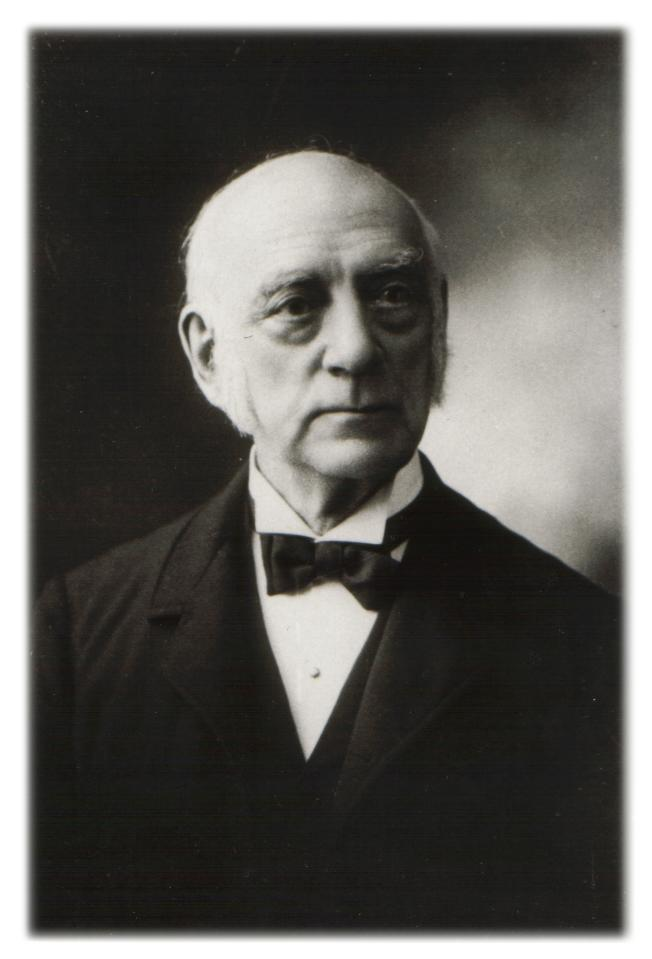
\includegraphics[scale=0.5,trim= 00 00 00 00]{../share/ei/James_Curtis_Hepburn.jpg}}
\\
\end{tabular}


         % label sec:Hepburn
% ---------------------------------------------------------------------------
\section{Hiragana - 平仮名} \label{sec:Hiragana}

TODO

{平仮名} {【ひらがな】}

               % label sec:Hiragana
\section{Homophone}\jsec{同音異語} 
% [o] LABEL
\label{sec:Homophone}
% [o] INDEX DESTINATION (DEF)
\ifor{homophone}{同音異語}{どうおん・いご}{Homophon}
% [o] INDEX TARGET
\ifor{Kanji}{漢字}{かんじ}{Kanji}

The linguistic term \textit{homophone} referenced the fact that some words in
language are pronounced equal but posses a different meaning. The spelling of
\textit{homophone}s may be equal or different.

\begin{center}\begin{tabular}{lllll}
\textbf{Language}&\textbf{word 1}&\textbf{meaning 1}&\textbf{word 2}&\textbf{meaning 2}\\\hline
German (same writing)      &Fliege&the insect  &Fliege &the bow tie \\
German (different writing) &aß    &ate (to eat)&Aas    &carrion     \\
English (same writing)     &does  &to do       &does   &plural of doe\\
English (different writing)&eight &8           &ate    &to eat       \\
\end{tabular}\end{center}

In general the meaning of \textit{homophone}s can be deducted from the context.
The is especially true if the spelling is different and if the
\textit{homophone} occurs while reading. It is more difficult but generally in
most cases possible to deduct the meaning also in spoken language. 

Homophones are rare in European languages like English or German. In Japanese
\textit{homophone}s are extraordinarily often. One reason\footnote{except the
one that people accept it and may even like it do nothing to reduce them} is
the mass import of Chinese words centuries ago by 'neglecting' the
pronunciation. While some Chinese word can be distinguished by pitch, they
become true \textit{homophone}s by flattening all pitches to only two. 

To give an extreme case, the following 22 \hyperref[sec:Kanji]{Kanji} words
(two \hyperref[sec:Kanji]{Kanji} each) are all pronounced /kikō/.

\begin{center}
{機構} {紀行} {稀覯} {騎行} {貴校} {奇功} {貴公} {起稿} {奇行} {機巧} {寄港}\\
{帰校} {気功} {寄稿} {機甲} {帰航} {奇効} {季候} {気孔} {起工} {気候} {帰港}
\end{center}

Even though they sound the same, in written language they can be differentiated. 

% TODO: what if the meaning is equal? Are they still homophones?
  % label sec:Homophone
% I
\section{Iroha}\jsec{伊呂波} 
% [o] LABEL
\label{sec:Iroha}
% [o] INDEX DESTINATION (DEF)
\ifor{Iroha}{伊呂波}{いろは}{Iroha}
% [o] INDEX TARGET
\ifor{Gojūonzu}{五十音図}{ごじゅうおんず}{50@50 Laute Tafel}
\ifor{Hiragana}{平仮名}{ひらがな}{Hiragana}

The word \textit{Iroha} stands for /iroha uta/ (\textit{Iroha} song) and is a
Japanese poem of the Heian era that contains all Kana words.  In contrast to
today it also contains more or less unuses letters, like /we/ or /wi/ and it do
not contain the newer /n/. Usual the poem is written in
\hyperref[sec:Hiragana]{Hiragana} from top to down.

\begin{center}
%\raisebox{10\height}{
%\framebox[20mm][r]{
\rotatebox{-90}{
\begin{minipage}{2.0cm}
    \setCJKfamilyfont{cjk-vert}[Script=CJK,RawFeature=vertical]{IPAPMincho}
    \renewcommand{\rubysep}{-0.5ex}
    \CJKfamily{cjk-vert}
いろはにほへとちりぬるをわかよたれそつねならむうゐのおくやまけふこえてあさきゆめみしゑひもせす
\end{minipage}
}
%}
%}
\end{center}

In this book the modern \hyperref[sec:Gojuonzu]{Gojūonzu} is used.

      % label sec:Iroha
% ---------------------------------------------------------------------------
\section{Katakana Iteration Marks} \label{sec:Iteration}

As with {漢字} {【かんじ】} also {片仮名} has a iteration mark.  「ヽ」 and its
{濁点} {【だくてん】} form {「ヾ」}. This can only be
found in rare cases. For example the personal name Misuzu 【みすゞ】might
contain this character. And since the difference between the second last
and the last mora is only a change in pronunciation the {濁点} is added.

In vertical writing exist another iteration marker {くの字点} {【くのじてん】}
which consist out of two characters {「〳」+「〵」} and the {濁点} form
is {「〴」+「〵」}

  % label sec:Iteration
% J
% K
% ---------------------------------------------------------------------------
\section{Kana - 仮名} \label{sec:Kana}

TODO
       % label sec:Kana

\ifor{Kanji}{漢字}{かんじ}{Kanji}

1300 years ago the first endeavours where undertaken to display the Japanese
language with the only known alphabet in the region, the Chinese writing
system. While the Japanese language where hardly suited for the writing system
it was an economical choice since the Chinese characters where well developed
at that time and introduced many new ideas in lexis. The 'borrowing' of Chinese
characters was not a one shot operation it took centuries and more then one
attempt. This long winded process led to the fact that some characters where
imported more then once from China from different times and different regions.
And because of this one Chinese character can have more then one pronunciation.
We hope that this will consolidate over the next centuries. Today this imported
characters are known as \textbf{Kanji} in Japan. \textbf{Kanji} is written
\textit{Hanzi} in Chinese and referencing the character from the Han period of
China. Even though today all Chinese based characters (and even some self
invented) are referenced nowadays as \textbf{Kanji}, it does not strictly mean
that they are only from the Han period.

A standard Japanese text do contain \textbf{Kanji}. To master the Japanese
language over a certain level and to over come the problem of personal
illiteracy (in Japan) it is highly encouraged to learn at least 600 to 800
characters. To become a fully literate member of the Japanese society 2000 to
2300 \textbf{Kanji} should be learned.

Today \textbf{Kanji} in written Japanese language are used for substantives/
nouns, verbs, adjectives and names.
                  % label sec:Kanji
% ---------------------------------------------------------------------------
\section{Katakana - 片仮名} \label{sec:Katakana}

At the same time as \hyperref[sec:Hiragana]{Hiragana}, also \textbf{Katakana}
letters where invented by simplifying the same Chinese characters used for
pronunciation.  However the look and feel of \textbf{Katakana} is more 'square'
not so 'rounded' as \hyperref[sec:Hiragana]{Hiragana}.

\textbf{Katakana} is used today for writing words of foreign origin and for
emphasizing (in commercials or \hyperref[sec:Manga]{Manga}) as well as word in
the fauna or flora.


   % label sec:Katakana
\section{Kunrei System}\jsec{訓令式ローマ字} 
% [o] LABEL
\label{sec:Kunrei}
\label{sec:KunreiSystem}
\label{sec:JapanSystemLatinLetters}
% [o] INDEX
\ifor{Kunrei system}{訓令式ローマ字}{くんれいろうまじ}{Kunrei System}
\ifor{Japan system Latin letters}{日本式ローマ字}{にほんしきろうまじ}{Lateinische Buchstaben des Japanischen Systems}
\ifor{Katakana}{片仮名}{かたかな}{Katakana}
\ifor{Gojūonzu}{五十音図}{ごじゅうおんず}{50 Laute Tafel}
\begin{tabular}{lr}
\begin{minipage}{9.6cm}

The modern \textbf{Kunrei} System {訓令式ローマ字} {【くんれいろうまじ】}  is
the official writing system of Japan. It was confirmed in 1994 by the Cabinet
and is available as ISO 3602:1989. The \textbf{Kunrei} System predecessor was
introduced 1985 by Dr. Aikitsu Tanakadatei ({田中舘愛橘}) as {日本式ローマ字}
{【にほんしきろうまじ】} (Nihon-/Nipponshikiromaji) and tries a more
systematical approach to map \hyperref[sec:Hiragana]{Hiragana} and
\hyperref[sec:Katakana]{Katakana} to equal Roman letters. The {五十音図}
{【ごじゅうおんず】} in the {訓令式ローマ字} is as follows:

\Link \href{http://en.wikipedia.org/wiki/Tanakadate_Aikitsu}{Tanakadate}

\end{minipage}
&
\raisebox{-.5\height}{
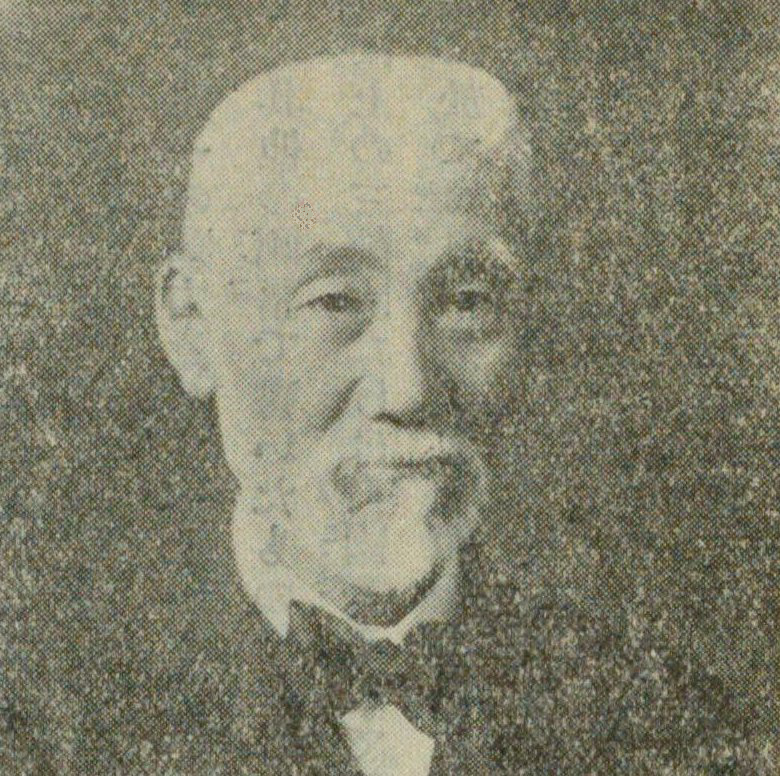
\includegraphics[scale=0.25,trim= 00 00 00 00]{../share/ei/Aikitsu_Tanakadate_r.jpg}}
\\
\end{tabular}


\Info{訓令式ローマ字 - Kunrei System}{
\begin{center}
\begin{tabular}{|c|c|c|c|c|}\hline
   a & i& u& e& o\\\hline
   ka&ki&ku&ke&ko\\\hline
   sa&si&su&se&so\\\hline
   ta&ti&tu&te&to\\\hline
   na&ni&nu&ne&no\\\hline
   ha&hi&hu&he&ho\\\hline
   ma&mi&mu&me&mo\\\hline
   ya&  &yu&  &yo\\\hline
   ra&ri&ru&re&ro\\\hline
   wa&  &  &  & o\\\hline
     &  &  &  & n\\\hline
\end{tabular}
\end{center}
}{true}

Even tough the system is official, many entities (like the train system) are
not using it. They use the Hepburn System.

The {訓令式ローマ字} is not part of this book. Please see \nameref{sec:Hepburn}
(on page \pageref{sec:Hepburn}) for the system in use.
          % label sec:Kunrei
% L
% M
% ---------------------------------------------------------------------------
\section{Manga - 漫画} \label{sec:Manga}

The Japanese version of comics is called \textbf{Manga} ({漫画} {【まんが】})
created on Japan or by Japanese authors. Some people say that \textbf{Manga} is
different from comics and deserve a name by its own. When \textbf{Manga} is
used in this book, then to distinguish it from comics in that sense that it is
written in Japanese posses a dynamic writing style\footnote{Conforming to a
style developed in Japan in the late 19th century.}  that is sometimes
challanging to its audience.

The term \textbf{Manga} for just Japanese comics is more used outside Japan. In
Japan all comics are referenced as \textbf{Manga} as well as with {コミック}
/komikku/ for all kinds of comics. The word \textbf{Manga} itself can be
translated as "whimsical drawings" or "impromptu sketches." and is used since
the late 18th century.


      % label sec:Manga
% ---------------------------------------------------------------------------
\section{Man'yōgana}\jsec{万葉仮名}
% [o] LABEL
\label{sec:Manyogana}
\label{sec:Manyoshu}
% [o] INDEX
\ifor{Man'yōgana}{万葉仮名}{まんようがな}{Man'yōgana}
\ifor{Man'yōshu}{万葉集}{まんようしゅう}{Man'yōshu}
\ifor{mora}{モーラ}{もーら}{Mora}
\ifor{Kanji}{漢字}{かんじ}{Kanji}
\ifor{Katakana}{片仮名}{かたかな}{Katakana}

The development of distinct Japanese writing begun 600 AD by writers and
scholars reducing some Chinese characters to its bare phonetic value. The
meaning of this characters where ignored. Around 760 a collection of Japanese
poetry was published, the \Link
\href{http://en.wikipedia.org/wiki/Man%27y%C5%8Dsh%C5%AB}{万葉集
【まんようしゅう】}, in which Chinese characters where uses as phonetic
letters. In regard to \textit{Man'yōshu} {万葉集} {【まんようしゅう】} the
characters are named {万葉仮名} {【まんようがな】}

The origin of the \textbf{Man'yōgana} script in poetry and art lead to some
problems in the understanding for the reader. Since the usage of phonetic
Chinese characters where mixed with regular Chinese characters and the
reasoning about which character to use was more form and shape aesthetic then
pragmatic, the meaning was difficult to grasp.

However the royal household or other scholars did not see a necessity to change
the status quo, because the high aim was to write poetry and other texts in
Chinese and \textbf{Man'yōgana} was considered appropriate only for notes,
diaries and love letters.

\Note{Note}{\footnotesize By the end of the 8th Century 970
\hyperref[sec:Kanji]{{漢字} {【かんじ】}} where used to pronounce the 90
\hyperref[sec:Mora]{morae}. This directly shows that there was no bijective map
between sound and character. For |ka| for example the following
\textbf{Man'yōgana} can be used {「可」}, {「何」}, {「加」}, {「架」},
{「香」}, {「蚊」}, {「迦」}. }

\newpage

The number of \textbf{Man'yōgana} from which \hyperref[sec:Katakana]{Katakana}
likely derived is smaller.  


\Hint{Man'yōgana used for creation of {片仮名} {【かたかな】}}{
\begin{center}
\begin{tabular}{|c||c|c|c|c|c|}\hline
 & a& i  & u  & e& o\\\hline\hline
-&阿&伊  &宇  &江&於\\\hline
k&加&機幾&久  &介&己\\\hline
s&散&之  &須  &世&曽\\\hline
t&多&千  &州川&天&止\\\hline
n&奈&仁  &奴  &祢&乃\\\hline
h&八&比  &不  &部&保\\\hline
m&末&三  &牟  &女&毛\\\hline
y&也&    &由  &  &與\\\hline
r&良&利  &流  &礼&呂\\\hline
w&和&井  &    &恵&乎\\\hline
*&尓&    &    &  &  \\\hline
\end{tabular}
\end{center}
}

The scientific term \textbf{Man'yōgana} is used by Western and Japanese
scientists. However it is not without critique. The term \textbf{Man'yōgana}
might lead to the illusion that it was a defined set of characters in use for
transcribing Chinese or writing Japanese texts or the second illusion that one
sound is represented by only  one \textbf{Man'yōgana}. Both is not true. First,
all Chinese Characters could in principle be used as \textbf{Man'yōgana} (and
therefore the term is basically useless). Actually the reason to chose one
character was sometimes just because out of aesthetic reasons, the shape or
some additional meaning. And second, normally many different
\textbf{Man'yōgana} (Chinese characters) where used for the same pronunciation
in the same text.  Making it efficient or easy was not the target of the
scholars using this kind of \hyperref[sec:PhoneticCharacter]{phonetic
characters} at that time.


\Link \href{http://en.wikipedia.org/wiki/Manyogana}{Man'yōgana}
\Link \href{http://en.wikipedia.org/wiki/Man%27y%C5%8Dsh%C5%AB}{万葉集}

  % label sec:Manyogana
% ---------------------------------------------------------------------------
\section{Mora - モーラ} \label{sec:Mora}

The concept of "mora"  (plural morae or moras; often symbolized μ) is used in
the science of linguistics. It describes a joint unit in pronunciation
(phonology) that constructs a syllable. The definition of a mora can vary.  In
Japanese the detection of morae is comparably simple. The world
{「チョコレート」} for example consist out of the following 5 morae
{「チョ」},{「コ」},{「レ」},{「ー」} and {「ト」} while it consist only out of
four \hyperref[sec:Syllable]{syllables} {(\hyperref[sec:Syllable]{音節}
【おんせつ】)}.

       % label sec:Mora
% N
% O
% ---------------------------------------------------------------------------
\section{Okurigana}\jsec{送り仮名}
% [o] LABEL
\label{sec:Okurigana}
\label{sec:Nokurigana}
% [o] INDEX
\ifor{okurigana}{送り仮名}{おくりがな}{Okurigana}
\ifor{katakana}{片仮名}{かたかな}{Katakana}
\ifor{kana}{仮名}{かな}{Kana}
\ifor{hiragana}{平仮名}{ひらがな}{Hiragana}
\ifor{kanji}{漢字}{かんじ}{Kanji}
\ifor{nokurigana}{ノくり仮名}{のくりがな}{Nokurigana}

The term \ivoc{okurigana}{送り仮名}{おくりがな}{Okurigana} in Japanese is
\textit{not} a script by its own as the name \hyperref[sec:Kana]{kana} suggest.
\textbf{Okurigana} are \hyperref[sec:Kana]{kana} but either
\hyperref[sec:Hiragana]{hiragana} or \hyperref[sec:Katakana]{katakana} that are
used to write the ending of words in most cases verbs. More precise
\textbf{okuriagna} are suffixes of \hyperref[sec:Kanji]{kanji}. After 1945 only
\hyperref[sec:Hiragana]{hiragana} are used to write \textbf{okurigana} while
before \hyperref[sec:Katakana]{katakana} was used.

\textbf{Okurigana} are the mandatory compromise using static Chinese letters to
write the Japanese language. Next to make \hyperref[sec:Kanji]{kanji} flexible
the other function is to mark the beginning are ending of words in sentences.

\textbf{Okurigana} have two purposes. (1) conjugate (a) verbs and (b)
adjectives. With very few exceptions\footnote{ {皮肉る} {【ひにくる】},
{牛耳る}  {【ぎゅうじる】} and {退治る} {【たいじる】}.}  \textbf{okurigana}
will only inflect \hyperref[sec:Kanji]{kanji} as \textit{kun'yomi}.  (2) Change
the meaning or reading of a \hyperref[sec:Kanji]{kanji} by different
\textbf{okurigana}.

\textit{Example: Okuriagana change the meaning (tense):}

\medskip
\begin{tabular}{ll}
\hspace{2cm}(1) {見る} {【みる】} & see \\
\hspace{2cm}(2) {見た} {【みた】} & saw \\
\end{tabular}

\medskip
In the above example the \textbf{okurigana} of (1) is \jquotesingleja{る} and the
\textbf{okurigana} of (2) is \jquotesingleja{た}.

\textit{Example: Okuriagana change the reading:}

\medskip
\begin{tabular}{ll}
\hspace{2cm}(1) {下さる} {【くださる】} & to give \\
\hspace{2cm}(2) {下りる} {【おりる】} &  to get off (a train for example)/ to descend \\
\hspace{2cm}(3) {下がる} {【さがる】} &  to dangle (intransitive)\\
\end{tabular}

\medskip
So in many cases the \textbf{okurigana} directly after the
\hyperref[sec:Kanji]{kanji} changes the meaning.

\textit{Example: Okuriagana change the meaning (transitivity) :}

\medskip
\begin{tabular}{ll}
\hspace{2cm}(1) {下がる} {【さがる】} &  to dangle (intransitive)\\
\hspace{2cm}(2){下げる} {【さげる】} &  to let off (transitive)\\
\end{tabular}

\medskip
As in the above case many Japanese verbs come in transitive and intransitive
pairs. The reading of the \hyperref[sec:Kanji]{kanji} is often shared.

\subsection*{Okurigana in the Middle}

\textbf{Okurigana} can also be found in the middle of Japanese words.

\textit{Example:}

\begin{center}\begin{tabular}{ll}
(1) {繰り返し} {【くりかえし】} &  to repeat\\
\end{tabular}\end{center}

\subsection*{Invisible Okuriagna - ノくり仮名}

The term \ivoc{nokurigana}{ノくり仮名}{のくりがな}{Nokurigana} was inspired by
the site \texttt{https://kanjidamage.com} but the writing was changed from
\hyperref[sec:Romaji]{rōmaji} to katakana+okurigana+kanji.  The
\hyperref[sec:Katakana]{katakana} \jquotesingleja{ノ} derives from the English
'no', and the word as such is a violation of the Japanese
\textbf{okurigana}\footnote{

Because \hyperref[sec:Katakana]{katakana} do not have \textbf{okurigana}. But
also in case there would be no violation the \jtl{o} of \jtl{okuri} would be
vilify to a honorific prefix and then to be ripped out by the 'no' in a very
non polite way.

} which describes a violation of \textbf{okurigana}.  Of course the term  is
not official, but quite funny in this case, that basically one should be very
angry with the fact that there are some Japanese words witch do have
\textbf{okurigana} but are not written (but of course pronounced!). The not so
funny part with those words is that if one knows the reading of the
\hyperref[sec:Kanji]{kanji} it is impossible to look them up in a dictionary.
So lets strike back and spread the word of the \textbf{nokurigana} -
{ノくり仮名}.

\begin{center}\begin{tabular}{ll}
(1) {取引} = {取り引き} {【と(り)ひ(き)】} &  Transaction\\
(2) {受付} = {受け付け} {【う(け)つ(け)】} &  Reception\\
\end{tabular}\end{center}


\Link \href{https://kanjidamage.com/tags/43}{https://kanjidamage.com/tags/43}








  % label sec:Okurigana
% P
\section{Phonetic Character - 表音文字} \label{sec:PhoneticCharacter}

In this document the term \textbf{Phonetic Character} ({表音文字}
{【ひょうおんもじ】}) refers genetically to a Chinese characters reading and
the usage of this character just for this purpose and \textit{not} for its
meaning. This common set expression has been used in avoidance of the term
\hyperref[sec:Manyogana]{Manyogana}. See the section \nameref{sec:Manyogana} on
page \pageref{sec:Manyogana} to understand the critique.

A \textbf{Phonetic Character} as to be distinguished from the linguistic term
\textit{phonogram} that describes a written character which represents a phonem
(speech sound) such as Latin alphabet or Japanese \hyperref[sec:Kana]{Kana}. 

 % label sec:PoneticCharacter
% Q
% R
% ---------------------------------------------------------------------------
\section{Radical}\jsec{部首}
% [o] LABEL
\label{sec:Radical}
% [o]  INDEX
\ifor{radical}{部首}{ぶしゅ}{Radikal}
\ifor{Kanji}{漢字}{かんじ}{Kanji}

A \textbf{radical} {部首} {【ぶしゅ】} is a root particle or character of a
Sino-Japanese character {漢字} {【かんじ】}. It is the most significant part of
a Sino-Japanese character. The concept was developed in China for Chinese
characters and is today known under the same name {部首} (pinyin: bùshǒu).

There is no general definition what a \textbf{radical} is or how many are
existing and it can vary a lot. The author of a dictionary has the power to
defined what a \textbf{radical} is and how much there will be in that
dictionary.

In more traditional Chinese or Japanese dictionaries a number of 214 or 244
\textbf{radicals} is quite common. However some modern approaches like the
\Link \href{http://www.hadamitzky.de/english/works_books.htm#KD}{\textit{The
Kanji Dictionary} of Marc Spahn and Wolfgang Hadamitzky from 1996} a totally
different number of 79 can be found.

\Note{Note}{\footnotesize Before buying a \hyperref[sec:Kanji]{Kanji}
dictionary, make sure that the \textbf{radical} system used suits your taste.
Sometimes it can be observed that Japanese dictionaries are stricter in the
definition of a \textbf{radical} because a given \hyperref[sec:Kanji]{Kanji}
can only be retrieved via exactly \textit{one} \textbf{radical}. While in many
Chinese dictionaries \textit{every} \textbf{radical} of a Chinese character can
be used to find it. The Japanese approach is of course good in terms of
systematic and didactic for learners, however it can take significant longer to
look up a character by \textbf{radical}.  }

    % label sec:Radical
\nopagebreak

\ithree{base table Rōmaji}{ローマ字}{Basistabelle Rōmaji}

\bigskip
\begin{center}
%\LARGE
\Huge

\begin{tabular}{c||c|c|c|c|c|}
&\textbf{a}&\textbf{i}&\textbf{u}&\textbf{e}&\textbf{o}\\\hline\hline
\textbf{-}  &a &i  &u  &e &o \\\hline
\textbf{k}  &ka&ki &ku &ke&ko\\\hline
\textbf{s}  &sa&shi&su &se&so\\\hline
\textbf{t}  &ta&chi&tsu&te&to\\\hline
\textbf{n}  &na&ni &nu &ne&no\\\hline
\textbf{h}  &ha&hi &fu &he&ho\\\hline
\textbf{m}  &ma&mi &mu &me&mo\\\hline
\textbf{y}  &ya&   &yu &  &yo\\\hline
\textbf{r}  &ra&ri &ru &re&ro\\\hline
\textbf{w}  &wa&   &   &  &o \\\hline
\textbf{{*}}&n &   &   &  &  \\\hline
\end{tabular}
\end{center}
     % label sec:Romaji
% S
\section{Space Character}\jsec{空白文字}
% [o] LABEL
\label{sec:SpaceCharacter}
% [o] INDEX DESTINATION (DEF)
\ifor{space character}{空白文字}{くうはく ・ もじ}{Leerzeichen}
% [o] INDEX TARGET
\ifor{katakana}{片仮名}{かたかな}{Katakana}
\ifor{kanji}{漢字}{かんじ}{Kanji}
\ifor{hiragana}{平仮名}{ひらがな}{Hiragana}
\ifor{rōmaji}{ローマ字}{ろーまじ}{Rōmaji}

The \ivoc{space character}{空白文字}{くうはくもじ}{Leerzeichen} in Western
(Latin letter based) languages is used to separate words. In antique texts a
separation of words was \textbf{not} common and those where difficult to read.
In the 7th century AD the word separation was introduced. In the beginning of
printed books the space wide was fixed and to archive this the width of the
letters where not fixed which produced an easy to read text body.

The invention of typewriters and computers destroyed this approach of
aesthetically advanced typography. The typewriters had still a fixed (too
large) space width but also fixed letters. While the computer on screen behave
not better as a typewriter in the beginning and in printing, the spaces are
variable and the letters are fixed, the opposite of the elegant book printing
of the 15th century AD.

With the invention of Unicode the \textit{space character} is not longer a
singularity. The Unicode fonts have now many\footnote{

To give an example: \texttt{U+2008} Punctuation Space, \texttt{U+2009} Thin
Space, ..., \texttt{U+FEFF} Zero Width No-Break Space, to just name a few.

} \textit{space characters}.

The Japanese computer fonts do have a \textit{space character}. Traditionally
more then one.  The most important \textit{space character} is the double wide
\textit{space character} which is exactly as wide as a
\hyperref[sec:Kanji]{kanji} character. And the single wide space character that
is as wide as \hyperref[sec:Romaji]{Rōmaji} or half wide
\hyperref[sec:Hiragana]{hiragana} or \hyperref[sec:Katakana]{katakana}.

However even though there is a \textit{space character} nowadays in Japanese
fonts it is \textbf{not} used to separate words from each other. Because of
this the word border can only be detected by heuristics and changes in scripts,
for example: \hyperref[sec:Katakana]{katakana} to \hyperref[sec:Kanji]{kanji},
\hyperref[sec:Hiragana]{hiragana} to \hyperref[sec:Kanji]{kanji},
\hyperref[sec:Katakana]{katakana} to \hyperref[sec:Hiragana]{hiragana} and so
on. Detecting words is a major task in learning Japanese.

The \textit{space character} in Japan is used to indent text to mark
paragraphs. To separate functional entities in the text like author from
heading.

As a matter of fact the \textit{space character} in modern Japanese plays a
very unimportant role.

This was not always so. In old Japanese there where an additional usage of
\textit{space characters} as \ivoc{ketsuji}{闕字}{けつじ}{Ketsuji} to leave
space in front of names of important persons or verbs to honor them.

\smallskip
\textbf{Example:}

\begin{center}\Padding\begin{tabular}{p{4cm}p{3cm}p{4cm}}
 \jquotesingleja{  上様} & {【うえさま】}      & Mister Ue \\
 \jquotesingleja{登  城} &  {【とう じょう】} & registered castle\\
\end{tabular}\end{center}
\smallskip

However this usage was abandoned in the Meiji era.

\Link \href{https://ja.wikipedia.org/wiki/%E9%97%95%E5%AD%97}{https://ja.wikipedia.org/wiki/闕字}

 % sec:SpaceCharacter
% ---------------------------------------------------------------------------
\section{Syllable - 音節} \label{sec:Syllable}

A \textbf{syllable} {音節}  {【おんせつ】}  is a phonetic building block for
words. It influences the rhythm of a spoken language. In Western languages a
\textbf{syllable} is made out of one or more letters. In Japanese it is often
one character (of \hyperref[sec:Kana]{Kana}), but not always. For a better
understanding of the Japanese it is important to understand the concept of
\hyperref[sec:Mora]{mora}.

\Link \href{http://en.wikipedia.org/wiki/Syllable}{Syllable}
\Link \href{http://ja.wikipedia.org/wiki/%E9%9F%B3%E7%AF%80}{音節}

   % label sec:Syllable
% T
% U
% V
% W
% X
% Y
% Z

          % 5 chap:Terminology

% === [ APPENDIX ] ============================================================
\appendix

% \input can not handle \jscript{}
\newcommand{\jTableKana}[2]{\jptab/#1#2}
%\newcommand{\jTablKanaJapaneseDefault}[1]{\jptab/#1JapaneseDefault}

%/\chapter{Katakana Tables}\jchap{{片仮名図} \label{chap:KatakanaTables}
%\chapter{\jscript{} Tables}\jchap{{\jsubtitlejapanese}図} \label{chap:{\jscript{}}Tables}
\chapter{\jscript{} Tables}\jchap{\jsubtitlejapanese{}図}\label{chap:KanaTables}
\ithree{\jtopic{}!tables}{平仮名図}{\jscript{}!Tabellen}

\section{\jscript{} Reference}\jsec{片仮名のレファレンス}
%\input{\jptab/\jscript{}Reference}

\section{\jscript{} Writing Reference}\jsec{片仮名の書くレファレンス}
%\input{\jppath{\jptab}{\jscript}{WritingReference}}
\begin{center}
\Padding
\begin{tabular}{|c||c|c|c|c|c|}\hline
       &\Huge    a &\Huge    i & \Huge   u &\Huge    e &\Huge    o\\\hline\hline
\Huge *&\Jletter{as}&\Jletter{is}&\Jletter{us}&\Jletter{es}&\Jletter{os}\\\hline
\Huge k&\Jletter{kas}&\Jletter{kis}&\Jletter{kus}&\Jletter{kes}&\Jletter{kos}\\\hline
\Huge s&\Jletter{sas}&\Jletter{shis}&\Jletter{sus}&\Jletter{ses}&\Jletter{sos}\\\hline
\Huge t&\Jletter{tas}&\Jletter{chis}&\Jletter{tsus}&\Jletter{tes}&\Jletter{tos}\\\hline
\Huge n&\Jletter{nas}&\Jletter{nis}&\Jletter{nus}&\Jletter{nes}&\Jletter{nos}\\\hline
\Huge h&\Jletter{has}&\Jletter{his}&\Jletter{fus}&\Jletter{hes}&\Jletter{hos}\\\hline
\Huge m&\Jletter{mas}&\Jletter{mis}&\Jletter{mus}&\Jletter{mes}&\Jletter{mos}\\\hline
\Huge y&\Jletter{yas}&\Jletter{s}&\Jletter{yus}&\Jletter{s}&\Jletter{yos}\\\hline
\Huge r&\Jletter{ras}&\Jletter{ris}&\Jletter{rus}&\Jletter{res}&\Jletter{ros}\\\hline
\Huge w&\Jletter{was}&\Jletter{s}&\Jletter{s}&\Jletter{s}&\Jletter{wos}\\\hline
\Huge n&\Jletter{ns}&\Jletter{s}&\Jletter{s}&\Jletter{s}&\Jletter{s}\\\hline
\end{tabular}
\end{center}


%\section{\jscript{} Hand Writing Reference}\jsec{片仮名の手で書くレファレンス}
%\input{../share/\jscript{}HandWritingReference}

\newpage

% ---------------------------------------------------------------------------
\section{Empty Gojūonzu for Training}\jsec{練習のため五十音図}
\ithree{empty Gojūonzu}{練習のため五十音図}{50@50 Laute Tafel!leer}
\ithree{Gojūonzu training}{練習のため五十音図}{50@50 Laute Tafel!trainieren}
\label{app:Leere50LauteTafel} Please fill in this table (as quickly as
possible) 10-20 times a day during the active learning phase.
\begin{center}
\Padding
\begin{tabular}{|c||c|c|c|c|c|}\hline
                   &\Huge    a &\Huge    i & \Huge   u &\Huge    e &\Huge    o\\\hline\hline
\Huge *&\Kletter{s}&\Kletter{s}&\Kletter{s}&\Kletter{s}&\Kletter{s}\\\hline
\Huge k&\Kletter{s}&\Kletter{s}&\Kletter{s}&\Kletter{s}&\Kletter{s}\\\hline
\Huge s&\Kletter{s}&\Kletter{s}&\Kletter{s}&\Kletter{s}&\Kletter{s}\\\hline
\Huge t&\Kletter{s}&\Kletter{s}&\Kletter{s}&\Kletter{s}&\Kletter{s}\\\hline
\Huge n&\Kletter{s}&\Kletter{s}&\Kletter{s}&\Kletter{s}&\Kletter{s}\\\hline
\Huge h&\Kletter{s}&\Kletter{s}&\Kletter{s}&\Kletter{s}&\Kletter{s}\\\hline
\Huge m&\Kletter{s}&\Kletter{s}&\Kletter{s}&\Kletter{s}&\Kletter{s}\\\hline
\Huge y&\Kletter{s}&\Kletter{s}&\Kletter{s}&\Kletter{s}&\Kletter{s}\\\hline
\Huge r&\Kletter{s}&\Kletter{s}&\Kletter{s}&\Kletter{s}&\Kletter{s}\\\hline
\Huge w&\Kletter{s}&\Kletter{s}&\Kletter{s}&\Kletter{s}&\Kletter{s}\\\hline
\Huge n&\Kletter{s}&\Kletter{s}&\Kletter{s}&\Kletter{s}&\Kletter{s}\\\hline
\end{tabular}
\end{center}


% ---------------------------------------------------------------------------
\newpage\section{\jscript{} Gojūonzu}\jsec{片仮名五十音図}
\ithree{\jtopic{}!Gojūonzu}{片仮名五十音図}{50@50 Laute Tafel!\jscript{}}
\input{\jptab/\jscript}

% ---------------------------------------------------------------------------
%\newpage\section{\jscript{} (bold) Gojūonzu}
%\input{\jptab/\jscript{}Bold.tex}

% ---------------------------------------------------------------------------
\newpage\JapaneseDejima\section{\jscript{} Font Dejima}\jsec{出島フォント片仮名}
\ithree{\jtopic{}!Font Dejima}{出島フォント片仮名}{\jscript{}!Font Dejima }
\input{\jptab/\jscript}\JapaneseDefault

% ---------------------------------------------------------------------------
\newpage\JapaneseFontA\section{\jscript{} YOzAb}\jsec{\jquotesingleja{YOzAb}の片仮名}
\ithree{\jtopic{}!YOzAb}{\jquotesingleja{YOzAb}の片仮名}{\jscript{}!YOzAb}
\input{\jptab/\jscript}\JapaneseDefault

% ---------------------------------------------------------------------------
\newpage\JapaneseFontB\section{\jscript{} YOzC90b}\jsec{\jquotesingleja{YOzC90b}の片仮名}
\ithree{\jtopic{}!YOzC90b}{\jquotesingleja{YOzC90b}の片仮名}{\jscript{}!YOzC90b}
\input{\jptab/\jscript}\JapaneseDefault

% ---------------------------------------------------------------------------
\newpage\JapaneseFontC\section{\jscript{} YOzE90b}\jsec{\jquotesingleja{YOzE90b}の片仮名}
\ithree{\jtopic{}!YOzE90b}{\jquotesingleja{YOzE90b}の片仮名}{\jscript{}!YOzE90b}
\input{\jptab/\jscript}\JapaneseDefault

% ---------------------------------------------------------------------------
\newpage\JapaneseFontD\section{\jscript{} AoyagiSosekiFont2}\jsec{\jquotesingleja{AoyagiSosekiFont2}の片仮名}
\ithree{\jtopic{}!AoyagiSosekiFont2}{\jquotesingleja{AoyagiSosekiFont2}の片仮名}{\jscript{}!AoyagiSosekiFont2}
\input{\jptab/\jscript}\JapaneseDefault

% ---------------------------------------------------------------------------
\newpage\JapaneseFontE\section{\jscript{} IPAGothic}\jsec{\jquotesingleja{IPAGothic}の片仮名}
\ithree{\jtopic{}!IPAGothic}{\jquotesingleja{IPAGothic}の片仮名}{\jscript{}!IPAGothic}
\input{\jptab/\jscript}\JapaneseDefault

% ---------------------------------------------------------------------------
\newpage\JapaneseFontF\section{\jscript{} IPAMincho}\jsec{\jquotesingleja{IPAMincho}の片仮名}
\ithree{\jtopic{}!IPAMincho}{\jquotesingleja{IPAMincho}の片仮名}{\jscript{}!IPAMincho}
\input{\jptab/\jscript}\JapaneseDefault

% ---------------------------------------------------------------------------
\newpage\JapaneseFontG\section{\jscript{} KanjiStrokeOrders}\jsec{\jquotesingleja{KanjiStrokeOrders}の片仮名}
\ithree{\jtopic{}!KanjiStrokeOrders}{\jquotesingleja{KanjiStrokeOrders}の片仮名}{\jscript{}!KanjiStrokeOrders}
\input{\jptab/\jscript}\JapaneseDefault

% ---------------------------------------------------------------------------
\newpage\JapaneseFontH\section{\jscript{} kiloji - B}\jsec{\jquotesingleja{kiloji - B}の片仮名}
\ithree{\jtopic{}!kiloji - B}{\jquotesingleja{kiloji - B}の片仮名}{\jscript{}!kiloji - B}
\input{\jptab/\jscript}\JapaneseDefault

% ---------------------------------------------------------------------------
\newpage\JapaneseFontI\section{\jscript{} KouzanBrushFontGyousyo}\jsec{\jquotesingleja{KouzanBrushFontGyousyo}の片仮名}
\ithree{\jtopic{}!KouzanBrushFontGyousyo}{\jquotesingleja{KouzanBrushFontGyousyo}の片仮名}{\jscript{}!KouzanBrushFontGyousyo}
\input{\jptab/\jscript}\JapaneseDefault

% ---------------------------------------------------------------------------
\newpage\JapaneseFontJ\section{\jscript{} MotoyaLMaru}\jsec{\jquotesingleja{MotoyaLMaru}の片仮名}
\ithree{\jtopic{}!MotoyaLMaru}{\jquotesingleja{MotoyaLMaru}の片仮名}{\jscript{}!MotoyaLMaru}
\input{\jptab/\jscript}\JapaneseDefault

% ---------------------------------------------------------------------------
\newpage\JapaneseFontK\section{\jscript{} SetoFont}\jsec{\jquotesingleja{SetoFont}の片仮名}
\ithree{\jtopic{}!SetoFont}{\jquotesingleja{SetoFont}の片仮名}{\jscript{}!SetoFont}
\input{\jptab/\jscript}\JapaneseDefault

% ---------------------------------------------------------------------------
\newpage\JapaneseFontL\section{\jscript{} TakaoMincho}\jsec{\jquotesingleja{TakaoMincho}の片仮名}
\ithree{\jtopic{}!TakaoMincho}{\jquotesingleja{TakaoMincho}の片仮名}{\jscript{}!TakaoMincho}
\input{\jptab/\jscript}\JapaneseDefault

% ---------------------------------------------------------------------------
\newpage\JapaneseFontM\section{\jscript{} VL Gothic}\jsec{\jquotesingleja{VL Gothic}の片仮名}
\ithree{\jtopic{}!VL Gothic}{\jquotesingleja{VL Gothic}の片仮名}{\jscript{}!VL Gothic}
\input{\jptab/\jscript}\JapaneseDefault

% ---------------------------------------------------------------------------
\newpage
\JapaneseMikachanPB\section{\jscript{} MikachanPB}\jsec{\jquotesingleja{MikachanPB}の片仮名}
\label{sec:\jscript{}MikachanPB}
\ithree{\jtopic{}!MikachanPB}{\jquotesingleja{MikachanPB}の片仮名}{\jscript{}!MikachanPB}
\input{\jptab/\jscript}\JapaneseDefault

% ---------------------------------------------------------------------------
\newpage\section{\jscript{} Total Table}\jsec{全部片仮名}
\ithree{\jtopic{}!total table}{全部片仮名}{\jscript{}!Tabelle komplett}
\input{\jTableKana{\jscript}{All}}
                % A chap:KanaTables
\chapter{Rōmaji Tables}\jchap{ローマ字図}
% [o] LABEL
\label{chap:RomajiTables}
\label{sec:RomajiTables}
% [o] INDEX
\ithree{Rōmaji tables}{ローマ字図}{Rōmaji Tabellen} % DESTINATION
\ifor{Gojūonzu}{五十音図}{ごじゅうおんず}{50@50 Laute Tafel} % TARGET

% ---------------------------------------------------------------------------
\section{Base Rōmaji Table}\jsec{ローマ字}
% [o] LABEL
\label{sec:BaseRomajiTables}
% [o] INDEX
\ithree{base Rōmaji tables}{一般ローマ字図}{Basis Rōmaji Tabellen} % DESTINATION
\ifor{Gojūonzu}{五十音図}{ごじゅうおんず}{50@50 Laute Tafel} % TARGET
\nopagebreak

\ithree{base table Rōmaji}{ローマ字}{Basistabelle Rōmaji}

\bigskip
\begin{center}
%\LARGE
\Huge

\begin{tabular}{c||c|c|c|c|c|}
&\textbf{a}&\textbf{i}&\textbf{u}&\textbf{e}&\textbf{o}\\\hline\hline
\textbf{-}  &a &i  &u  &e &o \\\hline
\textbf{k}  &ka&ki &ku &ke&ko\\\hline
\textbf{s}  &sa&shi&su &se&so\\\hline
\textbf{t}  &ta&chi&tsu&te&to\\\hline
\textbf{n}  &na&ni &nu &ne&no\\\hline
\textbf{h}  &ha&hi &fu &he&ho\\\hline
\textbf{m}  &ma&mi &mu &me&mo\\\hline
\textbf{y}  &ya&   &yu &  &yo\\\hline
\textbf{r}  &ra&ri &ru &re&ro\\\hline
\textbf{w}  &wa&   &   &  &o \\\hline
\textbf{{*}}&n &   &   &  &  \\\hline
\end{tabular}
\end{center}


% ---------------------------------------------------------------------------
\section{All Rōmaji}\jsec{全部ローマ字}
% [o] LABEL
\label{sec:CompleteRomajiTables}
% [o] INDEX
\ithree{complete Rōmaji tables}{全部ローマ字図}{komplette Rōmaji Tabellen} % DESTINATION
\ithree{Rōmaji}{ローマジ}{Rōmaji}

\LARGE

\begin{center}

\begin{tabular}{c||c|c|c|c|c||c|c|c|}
& \textbf{\large a}& \textbf{\large i}& \textbf{\large u}& \textbf{\large e}& \textbf{\large o}&
\textbf{\small ya}& \textbf{\small yu}& \textbf{\small yo}\\ \hline \hline 

\textbf{\large -}  & a &  i&    u&  e&  o&  ya&  yu&  yo\\ \hline 
\textbf{\large k}  & ka&  ki&  ku& ke& ko& kya& kyu& kyo\\
{\small g}         & ga&  gi&  gu& ge& go& gya& gyu& gyo\\ \hline 
\textbf{\large s}  & sa& shi&  su& se& so& sha& shu& sho\\
{\small z/j}       & za&  ji&  zu& ze& zo&  ja&  ju&  jo\\ \hline 
\textbf{\large t}  & ta& chi& tsu& te& to& cha& chu& cho\\
{\small d/j}       & da&  ji&  zu& de& do&    &    &    \\ \hline 
\textbf{\large n}  & na&  ni&  nu& ne& no& nya& nyu& nyo\\ \hline 
\textbf{\large h}  & ha&  hi&  fu& he& ho& hya& hyu& hyo\\
{\small b}         & ba&  bi&  bu& be& bo& bya& byu& byo\\
{\small p}         & pa&  pi&  pu& pe& po& pya& pyu& pyo\\ \hline 
\textbf{\large m}  & ma&  mi&  mu& me& mo& mya& myu& myo\\ \hline 
\textbf{\large r}  & ra&  ri&  ru& re& ro& rya& ryu& ryo\\ \hline 
\textbf{\large w}  & wa&    &    &   &  o&    &    &    \\ \hline 
\textbf{\large {*}}&  n&    &    &   &   &    &    &    \\ \hline 
\end{tabular}
\end{center}

              % B chap:RomajiTables
% +---------------------------------------------------------------------------+
% | content/english/chap/TechnicalTerms.tex                                   |
% |                                                                           |
% | List of Japanese technical terms with English and German translation.     |
% |                                                                           |
% | Version: 0.1.0                                                            |
% |                                                                           |
% | Changes:                                                                  |
% |                                                                           |
% | 0.1.0 2022-09-10 Christian Külker <c@c8i.org>                             |
% |     - Initial version release                                             |
% |                                                                           |
% +---------------------------------------------------------------------------+

\chapter{List of Japanese Technical Terms}
\label{chap:ListOfJapaneseTechnicalTerms}
\label{sec:JapaneseTechnicalTerms}
\jchap{日本専門用語リスト}
\ifor{Japanese technical terms}{日本専門用語}{にほんせんもんようご}{japanische Fachbegriffe}
\normalsize Ordered by Japanese \textbf{hiragana} pronunciation
\footnotesize\Padding
\begin{longtable}[c]{p{.5cm}p{3.5cm}p{4cm}p{3.5cm}p{3.5cm}}
\textbf{\#}&%
\textbf{Japanese}&%
\textbf{Hiragana}&%
\textbf{English}&%
\textbf{German}\\ \hline
% autoatically generated by: extract-ifor
\chapter{List of Japanese Technical Terms}
\label{chap:ListOfJapaneseTechnicalTerms}
\label{sec:JapaneseTechnicalTerms}
\jchap{日本専門用語リスト}
\ifor{Japanese Technical Terms}{日本専門用語}{にほんせんもんようご}{japanische Fachbegriffe}
\normalsize Ordered by Japanese pronunciation (Hiragana).
\footnotesize\Padding
\begin{longtable}[c]{p{.5cm}p{3.5cm}p{4cm}p{3.5cm}p{3.5cm}}
\textbf{\#}&\textbf{Japanese}&\textbf{Hiragana}&\textbf{English}&\textbf{German}\\ \hline
1&送り仮名&おくりがな&\hyperref[sec:Okurigana]{Okurigana}&Okurigana\\
2&踊り字&おどりじ&\hyperref[sec:RepitionMarkForKanjiAndKana]{repition mark for Kanji and Kana}&Wiederholungszeichen für Kanji und Kana\\
3&音節&おんせつ&\hyperref[sec:Syllable]{syllable}&Silbe\\
4&重ね字&かさねじ&\hyperref[sec:RepitionMark]{repition mark}&Wiederholungszeichen\\
5&片仮名&かたかな&\hyperref[sec:Katakana]{Katakana}&Katakana\\
6&片仮名の書き方&かたかな・の・かきかた&\hyperref[sec:TheWayToWriteKatakana]{The Way To Write Katakana}&Katakana Schreibweise\\
7&仮名&かな&\hyperref[sec:Kana]{Kana}&Kana\\
8&漢字&かんじ&\hyperref[sec:Kanji]{Kanji}&Kanji\\
9&空白文字&くうはく ・ もじ&\hyperref[sec:SpaceCharacter]{space character}&Leerzeichen\\
10&空白文字&くうはく・もじ&\hyperref[sec:SpaceCharacter]{space character}&Leerzeichen\\
11&くの字点&くのじてん&\hyperref[sec:Kunojiten]{Kunojiten}&Kunojiten\\
12&繰り返し記号&くりかえしきごう&\hyperref[sec:RepitionMark]{repition mark}&Wiederholungszeichen\\
13&訓令式ローマ字&くんれいろうまじ&\hyperref[sec:KunreiSystem]{Kunrei System}&Kunrei System\\
14&五十音図&ごじゅうおんず&\hyperref[sec:Gojuonzu]{Gojūonzu}&50 Laute Tafel\\
15&修正ヘボン式ローマ字&しゅうせい・へぼんしき・ろうまじ&\hyperref[sec:NewerHepburnSystem]{newer Hepburn System}&neueres Hepburn System\\
16&専門用語&せんもんようご&\hyperref[sec:Terminology]{Terminology}&Fachbegriffe\\
17&濁点&だくてん&\hyperref[sec:Dakuten]{Dakuten}&Dakuten\\
18&長音&ちょうおん&\hyperref[sec:Choon]{Chōon}&Chōon\\
19&同音異語&どうおん・いご&\hyperref[sec:Homophone]{homophone}&Homophon\\
20&特別カタカナ&とくべつかたかな&\hyperref[sec:SpecialKatakanaCharacters]{Special Katakana Characters}&Spezielle Katakana Zeichen\\
21&日本式ローマ字&にほんしきろうまじ&\hyperref[sec:JapanSystemLatinLetters]{Japan System Latin letters}&Lateinische Buchstaben des Japanischen Systems\\
22&日本専門用語&にほんせんもんようご&\hyperref[sec:JapaneseTechnicalTerms]{Japanese Technical Terms}&japanische Fachbegriffe\\
23&ノくり仮名&のくりがな&\hyperref[sec:Nokurigana]{Nokurigana}&Nokurigana\\
24&倍増母音&ばいぞうぼいん&\hyperref[sec:DoublingVowels]{doubling vowels}&Vokalverdopplung\\
25&半濁点&はんだくてん&\hyperref[sec:Handakuten]{Handakuten}&Handakuten\\
26&筆画&ひっかく&\hyperref[sec:Stroke]{Stroke}&Strich\\
27&筆画の種類&ひっかくのしゅるい&\hyperref[sec:StrokeTypes]{Stroke Types}&Strich Typen\\
28&表音文字&ひょうおんもじ&\hyperref[sec:PhoneticCharacter]{Phonetic Character}&Phonetisches Zeichen\\
29&標準ヘボン式ローマ字&ひょうじゅん・へぼん・ろまあじ&\hyperref[sec:OlderHepburnSystem]{older Hepburn System}&altes Hepburn System\\
30&平仮名&ひらがな&\hyperref[sec:Hiragana]{Hiragana}&Hiragana\\
31&部首&ぶしゅ&\hyperref[sec:Radical]{radical}&Radikal\\
32&振り仮名&ふりがな&\hyperref[sec:Furigana]{Furigana}&Furigana\\
33&ヘボン式&へぼんしき&\hyperref[sec:HepburnSystem]{Hepburn System}&Hepburn System\\
34&変体仮名&へんたいがな&\hyperref[sec:Hentaigana]{Hentaigana}&Hentaigana\\
35&漫画&まんが&\hyperref[sec:Manga]{manga}&Manga\\
36&万葉仮名&まんようがな&\hyperref[sec:Manyogana]{Man'yōgana}&Man'yōgana\\
37&万葉集&まんようしゅう&\hyperref[sec:Manyoshu]{Man'yōshu}&Man'yōshu\\
38&モーラ&もーら&\hyperref[sec:Mora]{mora}&Mora\\
39&読み仮名&よみがな&\hyperref[sec:Yomigana]{Yomigana}&Yomigana\\
40&ルビ&るび&\hyperref[sec:Rubi]{rubi}&Rubi\\
41&ローマ字&ろーまじ&\hyperref[sec:Romaji]{Rōmaji}&Rōmaji\\
\end{longtable}

\end{longtable}
            % C chap:JapaneseTechnicalTerms

% INDEX

\phantomsection
\addcontentsline{toc}{chapter}{Indices}\jindex{索引}
%\chapter{Indices}
\fontspec{FreeSans}
\normalsize

% OLD: multind
%\phantomsection
%\printindex{english}{English: Terms}\jsubindex{英語専門用語索引}
%\label{chap:EnglishIndex}
%\phantomsection
%\printindex{japanese}{Japanese: Index}\jsubindex{日本語専門用語索引}
%\label{chap:JapaneseIndex}
%\phantomsection
%\printindex{german}{Deutsch: Fachbegriffe}\jsubindex{独逸語専門用語索引}
%\label{chap:GermanIndex}

% NEW: imakeidx 2022-06-24
\phantomsection
\clearpage
\begingroup
\addcontentsline{toc}{section}{English: Terms}\jsubindex{英語専門用語索引}
% \fbox* settings to fix the code in ../share/makeindex/english.ist
\setlength{\fboxsep}{5pt}%
\setlength{\fboxrule}{0pt}%
\printindex[english]
\label{chap:EnglishIndex}
\endgroup

\phantomsection
\clearpage
\begingroup
\addcontentsline{toc}{section}{Japanese: Index}\jsubindex{日本語専門用語索引}
\printindex[japanese]
\label{chap:JapaneseIndex}
\endgroup

\phantomsection
\clearpage
\begingroup
\addcontentsline{toc}{section}{Deutsch: Fachbegriffe}\jsubindex{独逸語専門用語索引}
% \fbox* settings to fix the code in ../share/makeindex/german.ist
\setlength{\fboxsep}{5pt}%
\setlength{\fboxrule}{0pt}%
\printindex[german]
\label{chap:GermanIndex}
\endgroup

% === [ BACK  ] ===============================================================

\backmatter

\chapter{Attribution}
\label{chap:attribution}

\begin{itemize}

        \item[Page \pageref{fig:KatakanaOrigin}:] ~\ref{fig:KatakanaOrigin}
                ~\nameref{fig:KatakanaOrigin} (file
                \texttt{share/i/Katakana\_origine.svg}) 2007-01-14 by
                \textit{Pmx} licensed under GFDL 1.2 with no invariant sections
                and CC-BY-2.5
                \url{https://de.wikipedia.org/wiki/Datei:Katakana_origine.svg}


\end{itemize}





% English: “…” ‘…’
% German: „…“   ‚…‘   »…«     ›…‹
%---------------------------------------------------------------------
\chapter{GNU Free Documentation License}
\label{chap:gnufdl}

\footnotesize

%\label{label_fdl}


 \begin{center}

       Version 1.2, November 2002


 Copyright \copyright 2000,2001,2002  Free Software Foundation, Inc.

 \bigskip

     59 Temple Place, Suite 330, Boston, MA  02111-1307  USA

 \bigskip

 Everyone is permitted to copy and distribute verbatim copies
 of this license document, but changing it is not allowed.
\end{center}


\begin{center}
{\textbf\large Preamble}
\end{center}

The purpose of this License is to make a manual, textbook, or other
functional and useful document “free” in the sense of freedom: to
assure everyone the effective freedom to copy and redistribute it,
with or without modifying it, either commercially or noncommercially.
Secondarily, this License preserves for the author and publisher a way
to get credit for their work, while not being considered responsible
for modifications made by others.

This License is a kind of “copyleft”, which means that derivative
works of the document must themselves be free in the same sense.  It
complements the GNU General Public License, which is a copyleft
license designed for free software.

We have designed this License in order to use it for manuals for free
software, because free software needs free documentation: a free
program should come with manuals providing the same freedoms that the
software does.  But this License is not limited to software manuals;
it can be used for any textual work, regardless of subject matter or
whether it is published as a printed book.  We recommend this License
principally for works whose purpose is instruction or reference.


\section{APPLICABILITY AND DEFINITIONS}


This License applies to any manual or other work, in any medium, that
contains a notice placed by the copyright holder saying it can be
distributed under the terms of this License.  Such a notice grants a
world-wide, royalty-free license, unlimited in duration, to use that
work under the conditions stated herein.  The \textbf{“Document”}, below,
refers to any such manual or work.  Any member of the public is a
licensee, and is addressed as \textbf{“you”}.  You accept the license if you
copy, modify or distribute the work in a way requiring permission
under copyright law.

A \textbf{“Modified Version”} of the Document means any work containing the
Document or a portion of it, either copied verbatim, or with
modifications and/or translated into another language.

A \textbf{“Secondary Section”} is a named appendix or a front-matter section of
the Document that deals exclusively with the relationship of the
publishers or authors of the Document to the Document's overall subject
(or to related matters) and contains nothing that could fall directly
within that overall subject.  (Thus, if the Document is in part a
textbook of mathematics, a Secondary Section may not explain any
mathematics.)  The relationship could be a matter of historical
connection with the subject or with related matters, or of legal,
commercial, philosophical, ethical or political position regarding
them.

The \textbf{“Invariant Sections”} are certain Secondary Sections whose titles
are designated, as being those of Invariant Sections, in the notice
that says that the Document is released under this License.  If a
section does not fit the above definition of Secondary then it is not
allowed to be designated as Invariant.  The Document may contain zero
Invariant Sections.  If the Document does not identify any Invariant
Sections then there are none.

The \textbf{“Cover Texts”} are certain short passages of text that are listed,
as Front-Cover Texts or Back-Cover Texts, in the notice that says that
the Document is released under this License.  A Front-Cover Text may
be at most 5 words, and a Back-Cover Text may be at most 25 words.

A \textbf{“Transparent”} copy of the Document means a machine-readable copy,
represented in a format whose specification is available to the
general public, that is suitable for revising the document
straightforwardly with generic text editors or (for images composed of
pixels) generic paint programs or (for drawings) some widely available
drawing editor, and that is suitable for input to text formatters or
for automatic translation to a variety of formats suitable for input
to text formatters.  A copy made in an otherwise Transparent file
format whose markup, or absence of markup, has been arranged to thwart
or discourage subsequent modification by readers is not Transparent.
An image format is not Transparent if used for any substantial amount
of text.  A copy that is not “Transparent” is called \textbf{“Opaque”}.

Examples of suitable formats for Transparent copies include plain
ASCII without markup, Texinfo input format, LaTeX input format, SGML
or XML using a publicly available DTD, and standard-conforming simple
HTML, PostScript or PDF designed for human modification.  Examples of
transparent image formats include PNG, XCF and JPG.  Opaque formats
include proprietary formats that can be read and edited only by
proprietary word processors, SGML or XML for which the DTD and/or
processing tools are not generally available, and the
machine-generated HTML, PostScript or PDF produced by some word
processors for output purposes only.

The \textbf{“Title Page”} means, for a printed book, the title page itself,
plus such following pages as are needed to hold, legibly, the material
this License requires to appear in the title page.  For works in
formats which do not have any title page as such, “Title Page” means
the text near the most prominent appearance of the work's title,
preceding the beginning of the body of the text.

A section \textbf{“Entitled XYZ”} means a named subunit of the Document whose
title either is precisely XYZ or contains XYZ in parentheses following
text that translates XYZ in another language.  (Here XYZ stands for a
specific section name mentioned below, such as \textbf{“Acknowledgements”},
\textbf{“Dedications”}, \textbf{“Endorsements”}, or \textbf{“History”}.)
To \textbf{“Preserve the Title”}
of such a section when you modify the Document means that it remains a
section “Entitled XYZ” according to this definition.

The Document may include Warranty Disclaimers next to the notice which
states that this License applies to the Document.  These Warranty
Disclaimers are considered to be included by reference in this
License, but only as regards disclaiming warranties: any other
implication that these Warranty Disclaimers may have is void and has
no effect on the meaning of this License.



\section{VERBATIM COPYING}


You may copy and distribute the Document in any medium, either
commercially or noncommercially, provided that this License, the
copyright notices, and the license notice saying this License applies
to the Document are reproduced in all copies, and that you add no other
conditions whatsoever to those of this License.  You may not use
technical measures to obstruct or control the reading or further
copying of the copies you make or distribute.  However, you may accept
compensation in exchange for copies.  If you distribute a large enough
number of copies you must also follow the conditions in section 3.

You may also lend copies, under the same conditions stated above, and
you may publicly display copies.



\section{COPYING IN QUANTITY}



If you publish printed copies (or copies in media that commonly have
printed covers) of the Document, numbering more than 100, and the
Document's license notice requires Cover Texts, you must enclose the
copies in covers that carry, clearly and legibly, all these Cover
Texts: Front-Cover Texts on the front cover, and Back-Cover Texts on
the back cover.  Both covers must also clearly and legibly identify
you as the publisher of these copies.  The front cover must present
the full title with all words of the title equally prominent and
visible.  You may add other material on the covers in addition.
Copying with changes limited to the covers, as long as they preserve
the title of the Document and satisfy these conditions, can be treated
as verbatim copying in other respects.

If the required texts for either cover are too voluminous to fit
legibly, you should put the first ones listed (as many as fit
reasonably) on the actual cover, and continue the rest onto adjacent
pages.

If you publish or distribute Opaque copies of the Document numbering
more than 100, you must either include a machine-readable Transparent
copy along with each Opaque copy, or state in or with each Opaque copy
a computer-network location from which the general network-using
public has access to download using public-standard network protocols
a complete Transparent copy of the Document, free of added material.
If you use the latter option, you must take reasonably prudent steps,
when you begin distribution of Opaque copies in quantity, to ensure
that this Transparent copy will remain thus accessible at the stated
location until at least one year after the last time you distribute an
Opaque copy (directly or through your agents or retailers) of that
edition to the public.

It is requested, but not required, that you contact the authors of the
Document well before redistributing any large number of copies, to give
them a chance to provide you with an updated version of the Document.




\section{MODIFICATIONS}


You may copy and distribute a Modified Version of the Document under
the conditions of sections 2 and 3 above, provided that you release
the Modified Version under precisely this License, with the Modified
Version filling the role of the Document, thus licensing distribution
and modification of the Modified Version to whoever possesses a copy
of it.  In addition, you must do these things in the Modified Version:

\begin{itemize}
\item[A.]
   Use in the Title Page (and on the covers, if any) a title distinct
   from that of the Document, and from those of previous versions
   (which should, if there were any, be listed in the History section
   of the Document).  You may use the same title as a previous version
   if the original publisher of that version gives permission.

\item[B.]
   List on the Title Page, as authors, one or more persons or entities
   responsible for authorship of the modifications in the Modified
   Version, together with at least five of the principal authors of the
   Document (all of its principal authors, if it has fewer than five),
   unless they release you from this requirement.

\item[C.]
   State on the Title page the name of the publisher of the
   Modified Version, as the publisher.

\item[D.]
   Preserve all the copyright notices of the Document.

\item[E.]
   Add an appropriate copyright notice for your modifications
   adjacent to the other copyright notices.

\item[F.]
   Include, immediately after the copyright notices, a license notice
   giving the public permission to use the Modified Version under the
   terms of this License, in the form shown in the Addendum below.

\item[G.]
   Preserve in that license notice the full lists of Invariant Sections
   and required Cover Texts given in the Document's license notice.

\item[H.]
   Include an unaltered copy of this License.

\item[I.]
   Preserve the section Entitled “History”, Preserve its Title, and add
   to it an item stating at least the title, year, new authors, and
   publisher of the Modified Version as given on the Title Page.  If
   there is no section Entitled “History” in the Document, create one
   stating the title, year, authors, and publisher of the Document as
   given on its Title Page, then add an item describing the Modified
   Version as stated in the previous sentence.

\item[J.]
   Preserve the network location, if any, given in the Document for
   public access to a Transparent copy of the Document, and likewise
   the network locations given in the Document for previous versions
   it was based on.  These may be placed in the “History” section.
   You may omit a network location for a work that was published at
   least four years before the Document itself, or if the original
   publisher of the version it refers to gives permission.

\item[K.]
   For any section Entitled “Acknowledgements” or “Dedications”,
   Preserve the Title of the section, and preserve in the section all
   the substance and tone of each of the contributor acknowledgements
   and/or dedications given therein.

\item[L.]
   Preserve all the Invariant Sections of the Document,
   unaltered in their text and in their titles.  Section numbers
   or the equivalent are not considered part of the section titles.

\item[M.]
   Delete any section Entitled “Endorsements”.  Such a section
   may not be included in the Modified Version.

\item[N.]
   Do not retitle any existing section to be Entitled “Endorsements”
   or to conflict in title with any Invariant Section.

\item[O.]
   Preserve any Warranty Disclaimers.
\end{itemize}

If the Modified Version includes new front-matter sections or
appendices that qualify as Secondary Sections and contain no material
copied from the Document, you may at your option designate some or all
of these sections as invariant.  To do this, add their titles to the
list of Invariant Sections in the Modified Version's license notice.
These titles must be distinct from any other section titles.

You may add a section Entitled “Endorsements”, provided it contains
nothing but endorsements of your Modified Version by various
parties--for example, statements of peer review or that the text has
been approved by an organization as the authoritative definition of a
standard.

You may add a passage of up to five words as a Front-Cover Text, and a
passage of up to 25 words as a Back-Cover Text, to the end of the list
of Cover Texts in the Modified Version.  Only one passage of
Front-Cover Text and one of Back-Cover Text may be added by (or
through arrangements made by) any one entity.  If the Document already
includes a cover text for the same cover, previously added by you or
by arrangement made by the same entity you are acting on behalf of,
you may not add another; but you may replace the old one, on explicit
permission from the previous publisher that added the old one.

The author(s) and publisher(s) of the Document do not by this License
give permission to use their names for publicity for or to assert or
imply endorsement of any Modified Version.



\section{COMBINING DOCUMENTS}



You may combine the Document with other documents released under this
License, under the terms defined in section 4 above for modified
versions, provided that you include in the combination all of the
Invariant Sections of all of the original documents, unmodified, and
list them all as Invariant Sections of your combined work in its
license notice, and that you preserve all their Warranty Disclaimers.

The combined work need only contain one copy of this License, and
multiple identical Invariant Sections may be replaced with a single
copy.  If there are multiple Invariant Sections with the same name but
different contents, make the title of each such section unique by
adding at the end of it, in parentheses, the name of the original
author or publisher of that section if known, or else a unique number.
Make the same adjustment to the section titles in the list of
Invariant Sections in the license notice of the combined work.

In the combination, you must combine any sections Entitled “History”
in the various original documents, forming one section Entitled
“History”; likewise combine any sections Entitled “Acknowledgements”,
and any sections Entitled “Dedications”.  You must delete all sections
Entitled “Endorsements”.



\section{COLLECTIONS OF DOCUMENTS}


You may make a collection consisting of the Document and other documents
released under this License, and replace the individual copies of this
License in the various documents with a single copy that is included in
the collection, provided that you follow the rules of this License for
verbatim copying of each of the documents in all other respects.

You may extract a single document from such a collection, and distribute
it individually under this License, provided you insert a copy of this
License into the extracted document, and follow this License in all
other respects regarding verbatim copying of that document.




\section{AGGREGATION WITH INDEPENDENT WORKS}



A compilation of the Document or its derivatives with other separate
and independent documents or works, in or on a volume of a storage or
distribution medium, is called an “aggregate” if the copyright
resulting from the compilation is not used to limit the legal rights
of the compilation's users beyond what the individual works permit.
When the Document is included in an aggregate, this License does not
apply to the other works in the aggregate which are not themselves
derivative works of the Document.

If the Cover Text requirement of section 3 is applicable to these
copies of the Document, then if the Document is less than one half of
the entire aggregate, the Document's Cover Texts may be placed on
covers that bracket the Document within the aggregate, or the
electronic equivalent of covers if the Document is in electronic form.
Otherwise they must appear on printed covers that bracket the whole
aggregate.




\section{TRANSLATION}



Translation is considered a kind of modification, so you may
distribute translations of the Document under the terms of section 4.
Replacing Invariant Sections with translations requires special
permission from their copyright holders, but you may include
translations of some or all Invariant Sections in addition to the
original versions of these Invariant Sections.  You may include a
translation of this License, and all the license notices in the
Document, and any Warranty Disclaimers, provided that you also include
the original English version of this License and the original versions
of those notices and disclaimers.  In case of a disagreement between
the translation and the original version of this License or a notice
or disclaimer, the original version will prevail.

If a section in the Document is Entitled “Acknowledgements”,
“Dedications”, or “History”, the requirement (section 4) to Preserve
its Title (section 1) will typically require changing the actual
title.




\section{TERMINATION}



You may not copy, modify, sublicense, or distribute the Document except
as expressly provided for under this License.  Any other attempt to
copy, modify, sublicense or distribute the Document is void, and will
automatically terminate your rights under this License.  However,
parties who have received copies, or rights, from you under this
License will not have their licenses terminated so long as such
parties remain in full compliance.




\section{FUTURE REVISIONS OF THIS LICENSE}



The Free Software Foundation may publish new, revised versions
of the GNU Free Documentation License from time to time.  Such new
versions will be similar in spirit to the present version, but may
differ in detail to address new problems or concerns.  See
https://www.gnu.org/copyleft/.

Each version of the License is given a distinguishing version number.
If the Document specifies that a particular numbered version of this
License “or any later version” applies to it, you have the option of
following the terms and conditions either of that specified version or
of any later version that has been published (not as a draft) by the
Free Software Foundation.  If the Document does not specify a version
number of this License, you may choose any version ever published (not
as a draft) by the Free Software Foundation.



% German version gets English license

\end{document}
